%% History:
% Ondrej Guth (01.05.2015)
% Josef Hlavac & Tomas Zahradnicky (4.10.2010)
%  + Built on the FEL CVUT template by Daniel Sykora and Pavel Tvrdik
%  + Made for FIT CVUT
%  + Joined several chapters and cleaned
%  + Undefined references are typeset in an orange box to alert the writer!
%  + Index is automatically printed if the \usepackage{index} and
%    \newindex{default}{idx}{ind}{Index} lines are uncommented.
%
\documentclass[12pt,twoside,a4paper,final]{memoir}%two-page printing

\usepackage{a4wide}
\usepackage{fancyvrb}
\usepackage{datetime}
%\usepackage[T1]{fontenc}
\usepackage[czech,UKenglish]{babel}
\usepackage{graphicx}
\usepackage{rotating}
\usepackage{subcaption}
\usepackage{pdflscape}
\usepackage{placeins}
%\usepackage{setspace}
%\usepackage{epic} % Images drawn in Xfig, exported as .epic
\usepackage{longtable}
\usepackage{hyperref}
% \usepackage[hidelinks]{hyperref} %hyperlinks without colour boxes
% \usepackage[usenames]{color}
\usepackage{amssymb}
\usepackage{amsmath}
\usepackage{amsthm}

% \usepackage{tikz}

% Configuration of algorithm package
\usepackage[ruled,vlined]{algorithm2e}
\SetAlFnt{\small\sffamily}
\SetKwInput{KwInput}{Input}

% Helping user-defined macros
\newcommand{\ceil}[1]{\left\lceil #1 \right\rceil}
\newcommand\T{\rule{0pt}{2.3ex}}

%Command for parametrized cell in tabular
% usage : \multicell{WIDTH}{VSPACE}{TEXT}
\newcommand{\multicell}[3]{\parbox{#1}{\vspace{#2} #3 \vspace{#2}}}

%\usepackage[chapter]{algorithm}
% \usepackage{algpseudocode}
% \renewcommand{\algorithmicrequire}{\textbf{Input:}}
% \renewcommand{\algorithmicensure}{\textbf{Output:}}

%\usepackage{proof}
%\usepackage{latexsym}
%\usepackage{epsfig}
% \usepackage{subfigure}
% \usepackage{multirow}
%\usepackage{index}
%\newindex{default}{idx}{ind}{Index}

\usepackage[
nonumberlist, %do not show page numbers
acronym,      %generate acronym listing   -> Not used in this example (see line with %%% )
nomain,
numberedsection
% notoc,          %show listings as entries in table of contents
]      %use section level for toc entries
{glossaries}
\makeglossaries
\input phdmacro.tex %couple of macros for formatting the dissertation thesis,
                    %your personal and specific macros can be placed also there


\renewcommand{\labelitemi}{\(\circ\)}

\newenvironment{chapterintro}{\slshape}{\par}

\usepackage{etoolbox}
% fix TOC in memoir class
\makeatletter
\renewcommand{\@pnumwidth}{2em} 
\renewcommand{\@tocrmarg}{3em}
\patchcmd{\@endtheorem}{\@endpefalse}{}{}{}
\patchcmd{\endproof}{\@endpefalse}{}{}{}
\makeatother

%%%%%%%%%%%%%%%%%%%%%%%%%%%%%%%%%%%%%%%%%%%%%%%%%%%%%%%%%%%
% Configure the disertation thesis
%%%%%%%%%%%%%%%%%%%%%%%%%%%%%%%%%%%%%%%%%%%%%%%%%%%%%%%%%%%
\newcommand\DissTitle{Generation of High-Speed Network Device from High-Level Description}
%\newcommand\DissTitle{Methodology for Analysis of High-Speed Computer Networks}

\newcommand\FirstandFamilyName{Ing.\,Pavel Ben\'{a}\v{c}ek}
\newcommand\Email{pavel.benacek@fit.cvut.cz}
\newcommand\Month{Prague, \monthname}
\newcommand\Year{\the\year}
\newcommand\Supervisor{doc. Ing. Hana Kub\'{a}tov\'{a}, CSc.}
\newcommand\SupervisorAffiliation{
Department of Digital Design\\
Faculty of Information Technology\\
Czech Technical University in Prague\\
Th\'{a}kurova 9\\
160 00 Prague 6\\
Czech Republic}
%-> uncomment if you have a thesis co-supervisor
\newcommand\CoSupervisor{Ing. Viktor Pu\v{s}, Ph.D.}
\newcommand\CoSupervisorAffiliation{
CESNET a.l.e.\\
Zikova 4\\
160 00 Prague 6\\
Czech Republic}

\newcommand\PhDProgram{Informatics}
%\newcommand\PhDSpecialization{Informatics}
\newcommand\Department{Department of Digital Design}
\newcommand\Faculty{Faculty of Information Technology}
\newcommand\University{Czech Technical University in Prague}
\newcommand\Address{Th\'akurova 9, 160 00 Prague 6, Czech Republic}

\def\UrlBreaks{\do\/\do\-}

\maxsecnumdepth{subsubsection}
\setcounter{tocdepth}{2}
\makeheadstyles{FITthesis}{
	\chapterstyle{madsen}
	\setsecheadstyle{\Large\bfseries\sffamily}
	\setsubsecheadstyle{\large\bfseries\sffamily}
	\setsubsubsecheadstyle{\bfseries\sffamily}
}
\headstyles{FITthesis}

% \includeonly{
% 	tex/abstract
% 	,tex/acknowledgement
% 	,tex/introduction
% 	,tex/stateoftheart
% 	,tex/conclusions
% }


% List of acronyms
%\newacronym{DFA}{DFA}{deterministic finite automaton}
%\newacronym{NFA}{NFA}{nondeterministic finite automaton}
%\newacronym{FA}{FA}{finite automaton}.

% Insert hyphenation which will be applied to the document

\hyphenation{prog-ramma-bility}

\begin{document}

% Switch language to UKenglish .. just to be sure :)
\selectlanguage{UKenglish}

% Define block styles
\theoremstyle{definition}
\newtheorem{lemma}{Lemma}[section]
\newtheorem{theorem}[lemma]{Theorem}
\newtheorem{definition}[lemma]{Definition}
\newtheorem{preposition}[lemma]{Preposition}
\newtheorem{example}[lemma]{Example}
\newtheorem{corollary}[lemma]{Corollary}
\newtheorem{proposition}[lemma]{Proposition}
\newtheorem{property}[lemma]{Property}
\newtheorem{observation}[lemma]{Observation}
\theoremstyle{remark}
\newtheorem{notation}[lemma]{Notation}
\newtheorem{note}[lemma]{Note}

% allow @ to appear in macro names
% \makeatletter

% % produce undefined references in an orange box rather than just ??
% \def\@setref#1#2#3{%
%   \ifx#1\relax
%    \protect\G@refundefinedtrue
%    \nfss@text{\reset@font\bfseries\fcolorbox{black}{Orange}{??}}%
%    \@latex@warning{Reference `#3' on page \thepage \space
%              undefined}%
%   \else
%    \expandafter#2#1\null
%   \fi}
%

\frontmatter

\coverpagestarts

\pagestyle{ruled}

\chapter{Abstract}
%\chapter*{Abstract and Contributions}
%\addcontentsline{toc}{chapter}{\protect\numberline{}{Abstract and contributions}}

OpenFlow, as the most popular embodiment of Software-Defined Networking, provides a way
to network dataplane configuration at runtime. The OpenFlow specification strictly defines a set of supported protocols 
and actions for further processing of incoming traffic (i.e., switches are still mostly fixed). 
However, modern requirements on networking hardware have a dynamic
character and administrators of high-end networks want to react to new protocols, security threats,
novel approaches in traffic engineering, and so on. This isn't feasible with static network hardware and
leads to the need to replace the hardware more often than desired.

The aim of my \thesis{} is to provide the process of mapping from abstract language to the architecture of network device which is 
suitable for automatic generation and capable to hit processing speed of 100\,Gbps in single FPGA. 
The architecture of network device is based on predefined interfaces and modules which are connected to a high-speed processing pipeline.
The text provides details of transformation process to individual blocks of network 
device: parser, deparser, Match+Action table, Match+Action router and Match+Action group. 
The text also demonstrates the usage of High-Level Synthesis tools to provide a custom 
processing engine which is capable
to hit speed of 100\,Gbps. Finally, the text provides three use cases for demonstration of flexibility and easy extensibility
with new protocols and actions. Each use case was described in P4 language, translated to VHDL and tested in real hardware environment. 
The results show that generated devices are capable to meet throughput in range from 77.6 to 100\,Gbps.

%\bigskip
%\noindent The contributions of my \thesis{} are summarized in the following list:
%\begin{enumerate}
%    \item Introduction of modular architecture which is suitable for automatic generation of high-speed packet processing devices 
%    from abstract description.
%    \item Introduction of structure and mapping process for individual parts of generated packet processing device: 
%    Match+Action router, Match+Action table, parser and deparser. 
%    \item Tool, which generates the proposed architecture of packet processing device from abstract description in P4 language.
%    \item Experimental results of generated packet processing devices, including tests in real hardware platform.
%\end{enumerate}

\bigskip

\noindent\textbf{Keywords:}\\
\indent FPGA, High-Level Synthesis, Transformation, P4, SDN, High-Speed Computer Networks, 100\,Gbps, VHSIC Hardware Description Language.

%\vfill
%If you present in this thesis work achieved jointly with some other people except for your supervisor or co-supervisor, then this is a place to put their statements clarifying your qualitative and quantitative participation.
%For example,

%\noindent As a collaborator of {\FirstandFamilyName} and a co-author of his papers, I agree with {\FirstandFamilyName}'s authorship of the research results, as stated in this dissertation thesis.

%\bigskip\bigskip
%\begin{flushright}
%    \begin{tabular}{p{6cm}}
%           \dotfill\\
%           {\em Name Surname}
%    \end{tabular}
%\end{flushright}


% \newpage
\chapter*{Acknowledgements}

First of all, I would like to express my thanks to my dissertation thesis supervisors, 
Ing.\,Viktor Pu\v{s},\,Ph.D. and doc.\,Ing.\,Hana Kub\'atov\'a,\,CSc., for their support, valuable comments and guidance. 
They have been a constant source of encouragement and insight during my research and helped me with numerous problems and professional advancements.

Special thanks go to the staff of the Liberouter project, funded by CESNET, and the \Department{} of the Czech Technical University in Prague, 
who maintained a pleasant and flexible working environment for my research. 
I would like to express special thanks to the management of both institutions for providing of the funding for my research.
My research has been partially supported 
%skolni granty
by the Czech Technical University in Prague, grants No. SGS14/102/OHK3/042/14, No. SGS14/105/OHK3/1T/18, No. SGS15/122/OHK3/1T/18,
%granty cestnetu pod ministerstvem skolstvi
by the Ministry of Education, Youth, and Sports of the Czech Republic under research programs CESNET Large Infrastructure project No. LM2010005,
CESNET E-infrastructure project No. LM2015042,
%EU projekty
by the European Union in the context of the BEBA project (Grant Agreement: 644122)
%TACR projekty
and by the projects TA03010561, TH01010229 funded by the Technology Agency of the Czech Republic.

I would like to express thanks to my colleagues from the Liberouter group, namely Ing.\,Luk\'a\v{s} Kekely, Ing.\,Jan Ko\v{r}enek,\,Ph.D., 
Ing.\,Martin \v{Z}\'adn\'ik,\,Ph.D., Ing. Tom\'a\v{s} \v{C}ejka and others, 
for their valuable comments and motivation in my research.

My greatest thanks go to Petra and my family members for their infinite patience, care, love and support. 
Finally, I would like to greatly thank to my father MVDr.\,Zden\v{e}k Ben\'a\v{c}ek for his love, patience and amazing childhood because 
he suddenly died after the long disease on 3 December 2015 . 

%%%%%%%%%%%%%%%%%%%%%%%%%%%%%%%%%%%%%%%%%%%%%%%%%%%%%%%%%%%%%%%%%%%%%%%%%%%%%%%
% Original content                                                            %
%%%%%%%%%%%%%%%%%%%%%%%%%%%%%%%%%%%%%%%%%%%%%%%%%%%%%%%%%%%%%%%%%%%%%%%%%%%%%%%
%First of all, I would like to express my gratitude to my dissertation thesis
%supervisor, Dr. R\'obert~L\'orencz. He~has been a constant source of encouragement and insight during my research and helped me with numerous problems and professional advancements.  
%
%I would like to thank to Dr. \dots, and Prof. \dots for giving me \dots
%
%Special thanks go to the staff of the \Department{}, who maintained a pleasant and flexible environment for my research. I would like to express special thanks to the department management for providing most of the funding for my research. 
%% The following is important, as it refers to ``Vyzkumny zamer''.
%My research has also been partially supported 
%by the Ministry of Education, Youth, and Sport of the Czech Republic under research program MSM~6840770014, 
%by the Czech Science Foundation as project No. 201/06/1039, 
%by the Grant Agency of the Czech Technical University in Prague, grant No. SGS \dots, and
%by the \dots
%I would like to express thanks to my colleagues from \dots group, namely Mr. \dots, Ms. \dots, Dr. \dots, and others, for their valuable comments and proofreading.
%
%Finally, my greatest thanks go to my family members, for their infinite patience and care \dots


% \newpage
\vglue 6cm 
\begin{center}
\textbf{Dedication}
\end{center}
\vglue 2cm 
%It is very pleasant if you dedicate this piece of work to someone 
%who you especially like or who likes you.

\begin{center}
{\em To Petra and my family for their endless patience and support}
\end{center}

% or {\em To my parents},  

% or something similar.


% \newpage

\tableofcontents*
%------------------------------
%  LOF, LOT
%----------------------------------------------------------------------------------------------------------
% \newpage\addcontentsline{toc}{chapter}{\protect\numberline{}{List of Figures}}

\clearpage
\listoffigures*
% \newpage\addcontentsline{toc}{chapter}{\protect\numberline{}{List of Tables}}

\clearpage
\listoftables*
% \newpage\addcontentsline{toc}{chapter}{\protect\numberline{}{List of Algorithms}}

\clearpage
\listofalgorithms

% \newpage\addcontentsline{toc}{chapter}{\protect\numberline{}{Definitions, Notations and Abbreviations}}\input{tex/definitions.tex}
%----------------------------------------------------------------------------------------------------------
% \newpage
\setsecnumdepth{part}
\chapter{Abbreviations}

\noindent\textbf{Miscellaneous Abbreviations}\\

\begin{longtable}[l]{ll}
\textbf{CAM}     & Content Addressable Memory \\
\textbf{CESNET}  & Czech Educational and Scientific Network \\
\textbf{CPU}     & Central Processing Unit\\
\textbf{DFS}     & Depth-First-Search\\
\textbf{FPGA}    & Field Programmable Gate Array \\
\textbf{FSM}     & Finite State Machine \\
\textbf{HDL}     & Hardware Description Language\\ 
\textbf{HFE}     & Header Field Extractor \\
\textbf{HLL}     & High-Level Language \\
\textbf{HLS}     & High-Level Synthesis \\
\textbf{IPv4}    & Internet Protocol version 4\\
\textbf{IPv6}    & Internet Protocol version 6\\
\textbf{LAN}     & Local Area Network \\
\textbf{LPM}     & Longest Prefix Match \\
\textbf{LUT}     & Lookup Table \\
\textbf{MAC}     & Media Access Control \\
\textbf{MPLS}    & Multiprotocol Label Switching \\
\textbf{Mbps}    & Megabit per second \\
\textbf{NAT}     & Network Address Translation \\
\textbf{NIC}     & Network Interface Card \\
\textbf{NPU}     & Network Processing Unit \\
\textbf{P4}      & Programming Protocol-Independent Packet Processors \\
\textbf{PGR}     & Parser Graph Representation \\
\textbf{QoS}     & Quality of Service \\
\textbf{RX}      & Receiver \\
\textbf{SDM}     & Software Defined Monitoring \\
\textbf{SDN}     & Software-Defined Networking \\
\textbf{SW}      & Software \\
\textbf{TCAM}    & Ternary CAM \\
\textbf{TCP}     & Transport Control Protocol \\
\textbf{TX}      & Transmitter \\
\textbf{UDP}     & User Datagram Protocol \\
\textbf{VHDL}    & VHSIC Hardware Description Language \\
\textbf{VLAN}    & Virtual LAN\\
\textbf{VXLAN}   & Virtual Extensible LAN\\
\textbf{XML}     & Extensible Markup Language \\
\end{longtable}
\vskip 1cm

%\newpage

\noindent\textbf{Number Sets}\\

\begin{longtable}[l]{ll}
{$\mathbb N$} & Natural numbers set\\
{$\mathbb N_0$} & Natural numbers set $\cup\left\{0\right\}$\\
\end{longtable}
\vskip 1cm

\noindent\textbf{Common Mathematical Functions and Operators}\\

\begin{longtable}[l]{ll}
${\mathbf b}$              & Vector of $n$ elements, ${\mathbf b} = (b_0,b_1,b_2,\dots\,b_n )$\\
$b_{i}$                    & the $i^{\,\mathrm{th}}$ element of vector $\mathbf b$\\
$\text{len}({\mathbf b})$  & Number of elements of vector $\mathbf b$\\
$\max({\mathbf b})$        & Maximal element of vector $\mathbf b$\\
$\mathcal{O}(x)$           & The big $\mathcal{O}$ notation\\
$x\ mod\ n$                & The integer result of $x$ after division of $n$\\
$or$                       & Logical \textit{or} operation\\
$and$                      & Logical \textit{and} operation\\
$log_b\left( x \right)$    & The logarithm of a number $x$ to a base $b$\\
$a^b$                      & Power function where $a$ is a variable and $b$ is the exponent (or the power)\\
$\ceil{x}$                 & Round $x$ upwards. Return the smallest integer value that is not less than $x$\\
\end{longtable}
\vskip 1cm

%%%%%%%%%%%%%%%%%%%%%%%%%%%%%%%%%%%%%%%%%%%%%%%%%%%%%%%%%%%%%%%%%%%%%%%%%%%%%%%
%% Original content of the file %%%%%%%%%%%%%%%%%%%%%%%%%%%%%%%%%%%%%%%%%%%%%%%
%\textbf{Number Sets}\\
%
%\begin{tabular}{ll}
%{$\mathbb N$} & Natural numbers set\\
%{$\mathbb N_0$} & Natural numbers set $\cup\left\{0\right\}$\\
%{$\mathbb Z$} & Integer numbers set\\
%{$\mathbb Z_m$} & Least nonzero residue number set with a module of $m$\\
%{$\mathbb S_m$} & Symmetric residue number set with a module of $m$\\
%{$\mathbb Q$} & Rational numbers set\\
%{$\mathbb F_t$} & Floating point numbers set with a precision of $t$\\
%{$\mathbb R$} & Real numbers set
%\end{tabular}
%\vskip 1cm
%
%\noindent\textbf{Common Mathematical Functions and Operators}\\
%
%\begin{tabular}{ll}
%$10_2$ & Numbers' radices are designated with a subscript \\
%${\mathbf b}$ & Vector $\mathbf b$\\
%$b_{i}$ & the $i^{\,\mathrm{th}}$ element of vector $\mathbf b$\\
%${||\mathbf b||}$ & Norm of vector $\mathbf b$\\
%$\dim \mathbf b$ & Dimension of vector $\mathbf b$\\
%${\mathbf A}$ & Matrix $\mathbf A$\\
%$a_{i,\,j}$ & Element of matrix $\mathbf A$ at the $i^{\,\mathrm{th}}$ row, and the $j^{\,\mathrm{th}}$ column\\
%${\mathbf A^{-1}}$ & Inverse matrix to matrix $\mathbf A$\\
%${\mathbf A^T}$ & Transposed matrix to matrix $\mathbf A$\\
%${||\mathbf A||}$ & Norm of matrix $\mathbf A$\\
%$\cond \mathbf A$ & Condition number of matrix $\mathbf A$\\
%$\rank \mathbf A$ & Rank of matrix $\mathbf A$ --- how many independent rows/columns it has\\
%$\max\left\{a,\,b\right\}$ & Maximum of $a$ and $b$, $a$ when $a\geq b$, $b$ when $a<b$\\
%$\min\left\{a,\,b\right\}$ & Minimum of $a$ and $b$, $a$ when $a\leq b$, $b$ when $a>b$\\
%$O(x)$ & The big $O$ notation\\
%$\Theta(x)$ & The big $\Theta$ notation\\
%\end{tabular}
%\newpage
%
%\noindent\textbf{Mathematical Terminology}\\
%
%\begin{tabular}{ll}
%$Q$ & Number of prime number modules\\
%$M$ & A product of individual modules $M=\prod\limits_{i=1}^Q m_i$\\
%\dots & \dots\\
%\dots & \dots\\
%\dots & \dots\\
%\dots & \dots\\
%\end{tabular}
%\vskip 1cm
%
%\noindent\textbf{Miscellaneous Abbreviations}\\
%
%\begin{tabular}{ll}
%\textbf{FPU} & Floating Point Unit\\
%\textbf{\dots} & \dots\\
%\textbf{\dots} & \dots\\
%\textbf{\dots} & \dots\\
%\textbf{\dots} & \dots\\
%\end{tabular}
%\vskip 1cm

\setsecnumdepth{subsubsection}

% \mainbodystarts
\mainmatter

%\singlespacing
%\onehalfspacing
%\doublespacing
%\part{The Parameter Extraction Methodology}
%-----------------------
%  Chapters start here
\chapter{Introduction}
% \enlargethispage*{5pt}
\label{chap:introduction}

\section{Motivation}
%Brief description of the topic of the \thesis. A complete explanation of the topic shall be described within chapter 
%\ref{chap.stateoftheart} at page \pageref{chap.stateoftheart}.

% Tady popisu to, ze se pocitacove site rychle rozviji a je nutne na to reagovat. Proto se nehodi fixni hardware a software
% a hodne se pouziva konfigurovatelny HW zalozeny na FPGA. Nanestesti jsou HDL jazyky hodne slozite a tak je nemuze
% pouzivat odbornik na bezpecnost, matematik nebo sitovy admin.

OpenFlow \cite{openflow}, as the most popular embodiment of Software-Defined Networking (SDN), provides a way
to network dataplane configuration at runtime. The OpenFlow specification strictly defines a set of supported protocols 
and actions for further processing of incoming traffic (i.e., switches are still mostly fixed). 
However, modern requirements on networking hardware have a dynamic
character and administrators of high-end networks want to react to new protocols, security threats,
novel approaches in traffic engineering, and so on. 
This isn't feasible with static network hardware and leads to the need to replace the hardware more often than desired.

The fixed behavior of network devices isn't also suitable for further scaling of data centers because such technological solutions 
need to react to actual demands on network infrastructure. This need is an impulse for developers and manufactures of networking
hardware because they are motivated to provide highly reconfigurable platforms. The example of such solution is not only the OpenFlow switch
but also the Facebook's 6-pack \cite{FacebookSixPack} or Wedge \cite{FacebookWedge}. Both solutions are equipped with an ASIC chip
from Broadcom (for processing of network data at high-speed) and control software which is used as a substrate for implementation
of control logic. Such solution can be easily reprogrammed to serve as a router, switch, or network filter.

However, such devices cannot be later extended with support of novel classification, parsing, or packet processing functionality
at high-speed (i.e., they are highly reconfigurable but still fixed). 
Due to this, developers and manufactures of network hardware are motivated to equip network devices with reprogrammable chips like FPGAs. 
This platform connects the flexibility of software with parallel nature of hardware into one
compact package. 
There are also available hardware platforms \cite{combo-100g} for development of network applications, including frameworks for rapid 
prototyping \cite{NetCOPEWeb}.

The behavior of implemented functionality (or we can say hardware) is traditionally defined by the Hardware Description Language (HDL) which is not easy to 
learn. Moreover, development and debugging in such language can be time consuming. 
Due to this, higher abstractions like C/C++ or Python are being used. 
However, these abstractions typically suffer from performance issues and it isn't easy to describe high-speed network engine
in such language. On the other hand, these approaches are suitable for developers who don't have experience with HDL languages.
We feel that programming of FPGAs using the abstract description is very beneficial because user, developer, or network administrator can be
focused on network application and doesn't need to care about details of HDL language.

\section{Goals of the Dissertation Thesis}
% Tady se sepise par zakladnich prispevku moji prace (bude se pak opakovat v abstraktu, intru a zaveru)
The goals of my \thesis{} are summarized in the following list:
\begin{enumerate}
    \item To propose an architecture of network device which is suitable for automatic generation from an abstract description and is
    capable to implement high-speed packet processing devices.
    \item To identify and provide building blocks which are suitable for automatic generation and are capable 
    to work at high throughput.
    \item To introduce a transformation process for generation of a high-speed network device from the abstract description.
    \item To evaluate reached results from the view of flexibility, FPGA resources and throughput.
\end{enumerate}

\section{Structure of the Dissertation Thesis}
%The \thesis is organized into \dots chapters as follows:
%\begin{enumerate}
%\item \emph{Introduction}: Describes the motivation behind our efforts together with our goals. There is also a list of contributions of this \thesis. 
%\item \emph{Background and State-of-the-Art}: Introduces the reader to the necessary theoretical background and surveys the current state-of-the-art.
%\item \emph{Overview of Our Approach}: \dots
%\item \emph{Main Results}: \dots
%\item \emph{Conclusions}: Summarizes the results of our research, suggests possible topics for further research, and concludes the thesis.
%\end{enumerate}

The \thesis{} is organized into following chapters:
\begin{enumerate}
    \item \emph{Introduction} describes the motivation behind our efforts together with our goals. There is also a list of contributions 
    of this \thesis{}.
    \item \emph{Background and Related Work} introduces the reader to the necessary theoretical background and surveys the current 
    state-of-the-art in high-speed computer networks, together with languages for description of packet processing devices.
    \item \emph{Architecture of a Network Device} introduces possible targets, details of FPGA platform and it provides the overview of 
    our architecture of network device which is suitable for automatic generation from the abstract description. 
    The chapter also introduces our approach behind the mapping to the proposed architecture.
    \item \emph{Parser and Deparser Architecture} provides further details of input/output network blocks (parser and deparser) together with
    experimental results. 
    This chapter also discusses our transformation process from the abstract description to the architecture of these blocks.
    \item \emph{Match+Action Processing Pipeline} describes our architecture of match and action engine which is based on 
    mapping of parsed headers to executed actions. 
    The text also provides details of mapping from the abstract description to the proposed architecture of match and action engine. 
    The section also discusses the usage of current High-Level Synthesis (HLS) tool for description of processing engines at speed of 100\,Gbps.
    \item \emph{Use Case Study} introduces results for three use cases of generated pipeline, including Match+Action, to demonstrate the flexibility and
    easy extensibility with new actions and protocols.  
    This chapter provides results of required resources, throughput and possible speedup in development.
    \item \emph{Conclusion} summarizes the results of our research, suggests possible topics, and concludes the thesis.
\end{enumerate}

\chapter{Background and Related Work}
\label{chap:stateOfTheArt}

\begin{chapterintro}
The following section discusses the actual approaches in the area of packet parsing, classification and data processing. 
These operations are tightly bound and they need to be solved as effectively as possible because 
they are the keys for the effective and fast data processing in high-speed computer networks.
The section also introduces available abstract descriptions of packet processing devices. 
\end{chapterintro}

\section{Problem Statement}
% Tady se opet bude opakovat definice tri zakladnich operaci
% 1) Parsovani
% 2) Klasifikace
% 3) Obecne zpracovani (stavove zpracovani)
%
% Podrobny popis v odstavcich jednotlivych skupin
%
% Dale bude dobre najit vysokourovnove popisy pro popis sitoveho HW. Jsou v podstate dva Gorilla, Xilinx SDN, P4. 
% To je dulezite, protoze to budeme pouzivat jako vstup a melo by se dat namapovat na nas HW.

In this section, we define three fundamental network operation groups, which are the core components of each network device. 
From the packet processing point of view, we can define three groups of operations:
\begin{enumerate}
	\item Data Extraction/Packet Parsing
	\item Classification
	\item Data Processing (we will talk about stateful processing)
\end{enumerate}

The first group, Data Extraction, must precede all other groups like classification, routing, filtering of incoming traffic, and so on. 
Each incoming packet must pass through some sort of parsing block to understand what is transferred inside the network packet. 
The examined data is then used in next stages which are related to classification or 
data processing. Therefore, the parsing is the first action which is performed on incoming network packet and it has to be carefully 
designed to support the expected packet rate of network interface. 
For example, the maximal packet rate for 10\,Gbps Ethernet with minimal packet length (64 bytes) equals to 1,488,096 packets per second. 
The network device should be able to process it without any problems. 
It can be otherwise a bottleneck of the system. A simple parsing example can be extraction of the IP address, TCP ports, or MAC address.

Classification is tightly bound to packet parsing and it is typically the second operation in the packet processing chain. 
The packet classification means the categorization of incoming packets into classes. 
The extracted protocol fields form an identifier, which is used for searching of processing rule. 
Rule is typically stored in a database of rules. 
This database is searched with packet identifier for the best matching record. 
Matched rule contains the identifier of the action, which is to be performed on the packet. 
For example, the network switch extracts the destination MAC address which is used for searching of an output port. 

The last stage of the packet processing is the Data Processing block. This block is typically designed to perform some operations like data changing, 
advanced filtering based on pattern matching, and so on. 
This stage of packet processing typically accepts read rule from the classification and 
parsing stage to perform a predefined operation which can be set from a software tool or it can be hard-wired in the networking device. 
The graphical representation of 
the packet processing concept is shown in Fig.~\ref{fig:packetProc}. 
In some cases, we can have more classification and action stages to implement more complex operations
like reaction to modified set of header fields (e.g., filtering of traffic behind NAT) and so forth.

\begin{figure}[ht]
	\centering
	
\includegraphics[width=\textwidth]{chapters/pic/frame_data_process}
	\caption{Base packet processing pipeline.}
	\label{fig:packetProc}
\end{figure}


\section{Fundamental Network Operations}
% Napsat, ze ted budeme mluvit o state-of-the-art jednotlivych skupin s ohledem i na pripadnou praci v oblasti popisu
% pomoci high-level urovne. Hlavne se tu bude mluvit o resenich, ktere jsou nejvetsim prinosem v jednotlivych oblastech

The following text describes the current state-of-the-art of briefly introduced groups from the packet processing point of view. 
We introduce the cutting edge solutions because they are the starting point for our further research.

\subsection{Parsing}
\label{sec:parsing}
% State of the art pro parsovani

Network communication is divided into layers. Each layer has some task which is required for success delivery of network data.
The typical structure of a packet consists of a stack of protocol headers and payloads. 
Each protocol adds its own protocol header which is understandable 
by the same network layer on the other device. This is shown in Fig.~\ref{fig:osi}. The main task of the packet parsing is the extraction of 
protocols headers, which are added during transition of the conceptual OSI model. Typical extracted headers are IPv4 \cite{RFCIP},
IPv6 \cite{RFCIP6} , TCP and UDP \cite{RFCTRANS}.  

\begin{figure}[t]
    \centering
    
\includegraphics[scale=0.6]{chapters/pic/osi}
    \caption{Layered OSI Model; It is a conceptual model of network communication. Each layer has some task which is important for successful 
        data delivery between network services. The figure also introduces examples of typical layer protocols.}
    \label{fig:osi}
\end{figure}

As we mention in previous section, the Data Extraction is important operation of packet processing because it is typically used at each
point of network infrastructure like routers, switches, firewalls, and so on. 
Moreover, there are requests for more complex and non-trivial packet parsing. It is also the key operation for packet classification 
because results from this stage are used for searching for the best matching record.
The problem is still getting harder because the speed of network lines and parsing requirements
are still changing very dramatically. 
The main reason for this dramatic change is a growing number of communication protocols, which leads to more complicated protocol stack. 
This can be demonstrated on parsing of TCP protocol \cite{RFCTRANS} in Fig.~\ref{fig:PacketHeaderArrangement}. 
In our example, we introduce three Ethernet frames with different protocol stacks. 
This protocol arrangement leads to three various starting offsets of TCP protocol which have to be supported by the parser.
Moreover, the situation gets more complicated with Virtual Extensible LAN (VXLAN) \cite{RFCVXLAN}. 
The network virtualization technology is used to solve scalability problems in the area of cloud computing. 
It is similar to classic VLAN technology \cite{ieee2003vlan} but it encapsulates the network packets into UDP (instead of the MAC-based Ethernet frames).
The extended encapsulation leads to higher requirements on parser. 
From historical point of view, we can define two groups of parser implementation --- software and hardware based parsers.

Software based parsers are common and cheap variant of network parsers. The main component is typically the processor which 
extracts interesting data from incoming packets. 
Parser is typically a computer program which implements this functionality. This approach is also used in these days --- mainly for lower network 
speeds because the final solution is cheap and fast enough for this kind of packet processing. 
The big advantage of this solution is the flexibility of packet parser because we can react to current needs 
(parser can be easily replaced by new implementation).

\begin{figure}[t]
    \centering
    
\includegraphics[scale=0.78]{chapters/pic/HeaderParsingExample}
    \caption{The example of packet header arrangement; Number represents the protocol's offset.}
    \label{fig:PacketHeaderArrangement}
\end{figure}

The second group, hardware based, is more powerful solution which is able to process much higher throughput. 
All modern high-speed network devices contains some special kind of hardware accelerated network parser. 
The disadvantage of this solution is slower development and higher cost.
There are implementation platforms like structured ASICs or FPGA circuits. 
The FPGA platform is very popular because of its flexibility, programmability and speed. 
However, hardware based parser is much harder to develop and maintain than the software version with same functionality. 
This group of network parsers still faces some challenges to solve. 
The next section describes the main approaches of hardware based packet parsers.

Braun et al. \cite{Braun02protocolwrappers} follow the idea of the layered OSI network model. 
They introduced a hardware based framework of hand-written wrappers with onion-like structure. 
For example, the parsing of the IP and UDP protocols consists of parsing of the Ethernet frame, parsing of the IP address and parsing 
of the UDP protocol. However, the detailed description of the interface is not given in the text. The FPGA implementation is able to achieve the 
throughput of 2.6\,Gbps and it is unclear how the result scales for wider data paths (i.e., higher transfer rates).

Research in this area is very intensive and researches are focused on the usage of the High-Level Synthesis (HLS). 
The HLS is typically the transformation from a higher level description to a lower level description. 
For example, Handel-C is very similar to C language. 
The HLS description is transformed to the HDL (Hardware Description Language) which is typically used for programming of FPGA circuits. 
There is a general result for the HLS approach which was given by Dedek et al. in \cite{DedekHLS}. They investigated three different realizations of
the same block. There is the comparison
of two different realizations in embedded processors (software implementation in customized 16-bit RISC and soft-core $MicroBlaze^{TM}$ processor) 
and specialized hardware based implementation with usage of Handel-C language. 
The comparison was made from different points of view: the development time, 
the estimated frequency and the occupied area. 
This work demonstrates that usage of processors gives poor results. The average throughput equals to 712\,Mbps in 
the case of custom RISC processor, 83\,Mbps for the $MicroBlaze^{TM}$ and 1454\,Mbps for the Handel-C implementation. 
The second important demonstration comes from the usage of the HLS --- the throughput and short development time can be obtained by 
usage of the higher language (Handel-C in Dedek's example).

Kobiersky et al. \cite{Kobiersky} introduce the packet header analysis and field extraction for multigigabit networks. 
The architecture for packet header processing is generated from XML protocol scheme. More than 20\,Gbps throughput can be achieved using less 
than 5000 slices of Virtex-5 FPGA.
Maximal frequency depends on the internal crossbar which doesn't scale well for wider data paths. 
However, it is the important result which shows the approach of
High-Level Synthesized network parsers in high-speed network area because it allows us to dynamically react to new network protocols. 
Unfortunately, this approach is harder to use in faster networks (like 40 and 100\,Gbps). 

A good example of HLS usage was given by Attig and Brebner \cite{AttigBrebner}. 
They introduce a PP language --- a simple high-level language for description
of packet parsing algorithms in an implementation-independent manner. 
The PP language describes the structure of packet headers and methods which define parsing rules.
The paper presents the implementation for modern FPGA which is able to accommodate high-speed network processing. 
Proposed system scales from 1 to 400\,Gbps network speeds on Virtex-7 FPGA. 
The architectural structure of the Brebner's parser is massive microcode controlled pipeline 
which consumes about 10\% of Virtex-7 resources for 1024 bits wide datapath for most common set of supported protocols 
(Ethernet, VLAN, MPLS, IPv4, IPv6, TCP and UDP). Typical disadvantage of microcode controlled solutions
is higher latency compared to pure hardware implementations. In this case, the latency varies from 292 to 548 ns.
This is inconvenient in some applications like stock exchange algorithms where the latency is crucial.  

Pu\v{s} et al. \cite{PusKekelyHfem2} proposed a novel architecture of a pipelined packet parser for FPGA based solutions, which offers 
low latency in addition to high throughput. 
These two parameters can be tuned to the needs of a particular application. Usage of such solution is very wide. The parser is 
hand-optimized thanks to the direct implementation in VHDL. 
The parser consists of analyzing blocks for variety of protocols like IPv4, IPv6, MPLS, and so on. 
Each block performs the analysis of one protocol --- it follows the main idea of layered OSI network model which was discussed in previous text. 
The communication interface of parsing blocks is generally defined and it can be used for accommodation of new protocols.
The \textit{Generic Protocol Parser Interface} (GPPI) consists of the input information which is 
needed for parsing of single protocol. The GPPI's output interface includes the parsed data and information for the next analyzer block. 
Unfortunately, the current implementation doesn't contain any HLS support despite the structure of parser is regular which makes it suitable for 
transformation from general description of parsing process. 
The parser consumes about 1.19\% of Virtex-7 FPGA resources to achieve the throughput over 100\,Gbps and 4.88\% to achieve the throughput 
over 400\,Gbps for typical set of supported protocols.

\subsection{Classification}
\label{sec:classification}
% State of the art pro klasifikaci

%Balasaheb and Kulkuhari \cite{ClasBalaAgar2013} have proposed four main groups of packet classification approaches: exhaustive search, 
%decomposition, decision tree and hierarchical-trie. 
The packet classification can be viewed as a geometrical problem of multi-dimensional discrete space searching. 
Each dimension represents one parameter which is used for the classification. 
For example, the most common classification is using five dimensions --- source and destination IP 
addresses, source and destination ports and type of transport protocol. If we combine all these parameters together, we get a 
five-dimensional search space where each point defines one packet (i.e., one combination). 
We can assign a rule to each point (or points) of given discrete space. 
The process of packet classification, from all rules containing (or we can say matching) the packet, selects one rule with the highest priority. 
The example of geometrical representation of multi-dimensinal classification is shown in Fig.~\ref{fig:GeometricRepresentationOfMultiSearchSpace}.

\begin{figure}[t]
    \centering
    \includegraphics[scale=1.2]{chapters/pic/SearchSpaceExample}
    \caption{Geometrical representation of multi-dimensional search space; Asterisk (*) represents any possible bit suffix.}
    \label{fig:GeometricRepresentationOfMultiSearchSpace}
\end{figure}

Any searching problem can be solved by searching through all available entries. We can identify two approaches --- sequential and parallel.
The first group, sequential approach, is performed by comparing the parsed headers with all the entries in the list (memory). 
The disadvantage of this approach is slow search for large set of rules because the asymptotic complexity of the 
linear probing is $\mathcal{O}(n)$. 
We can use a Ternary CAM (TCAM) engine which is used in product devices for parallel multi-dimensional packet classification. 
TCAM is a specialized memory organized in rows. Each row is composed of number of simple memory cells, where each cell can be set to three
different values 0,1 and x (\textit{don't care}). The row matches the lookup key if memory cells with 0 and 1 are equal to the corresponding bit
of lookup key. The \textit{don't care} positions are ignored, both values (0 or 1) are allowed. 
This memory is capable to match all rows in parallel. However, the complexity, cost and power consumption grows with a number of inserted rules. 
More details about this approach can be found in \cite{PusPhd}.

The decomposition based methods derive the result of classification by aggregating the individual results from searched domains, 
where the Cartesian product is typically used during the aggregation phase.
These methods offer high throughput but require
a big amount of storage space. The primary challenge is how to efficiently aggregate the results of the single field searches. 
The required storage space can be reduced by usage of pseudorules which minimize the result of the Cartesian products. It was introduced 
by Dharmapurikar et al. in \cite{DharmapurikarMSCA}.
The pseudorule is a generated rule which handles situations for packets which are not directly defined by the rule but it is needed to
obtain the correct result of the classification. However, this set of rules and pseudorules can be quite large. 
For the minimization of generated pseudorules, the Prefix Filtering Classification and Prefix Coloring Classification algorithms were 
introduced  by Pu\v{s} in \cite{PusPhd}. These approaches are able to minimize and eliminate a big amount of pseudorules
which leads to effective hardware implementation, capable to accommodate more rules and needed pseudorules. 
However, the detailed description of pseudorule concept is out of scope of this work.

Most of the classification architectures and approaches are based on direct mapping of this problem to decision trees. 
\textit{HiCuts} \cite{And99HiCuts} and \textit{HyperCuts} \cite{SingHyperCuts} are the main representatives of this approach. 
They construct a decision tree where inner tree nodes divide the space by hyperplanes 
into subspaces (e.g., it "cuts" the space into small subspaces which will be searched for the rule). 
The \textit{HyperCuts} algorithm is faster because it allows cutting on 
multiple fields per one step. However, the depth of the tree depends on a particular set because the worst case 
represents the longest path from a root to a leaf. 
The throughput strongly depends on the passed rule set (i.e., generated tree).  

Yuaxuan  et al. \cite{YaxuanFongClassification100andBeyond} introduce a tree based multi-dimensional packet classification on FPGA which is 
capable to process traffic at speed of 100\,Gbps. They used the \textit{HyperSplit} \cite{YaxuanHyperSplit} algorithm for building of optimized
\textit{k}-d classification tree. The algorithm uses heuristic for selection of most efficient splitting point on a specific protocol field. 
The paper also discusses the architecture and mapping of \textit{HyperSplit} tree to the FPGA implementation with some optimizations for 
accommodation of more classification rules. The proposed architecture is able to classify 10K rules at speed of 118\,Gbps on Virtex 6 FPGA.

Fong et al. \cite{FongWangParasplitTerabitClassification} introduce another tree based classification approach which is capable to 
hit terabit speeds. Authors introduce the \textit{ParaSplit} algorithm which uses a rule set partitioning algorithm.
The algorithm is based on range-point conversion to reduce the overall memory requirements. Authors also optimize rule partitioning 
by applying of Simulated Annealing technique. They implement the architecture for FPGA which allocates separate search engine
for each created set. Therefore, the architecture uses the native parallelism for searching of the most suitable rule in more sets in the same time.
One proposed engine is able to process 10K rules at speed of 120\,Gbps on Virtex 5 FPGA. The terabit classification is possible thanks to 
instantiation of more search engines on single chip which allows distribution of incoming traffic.

The Grid-of-Tries \cite{SrinivasanGridOfTries} is the example of hierarchical-trie approach. 
It is optimized for two dimensions but it can be extended for more dimensions. 
The algorithm uses an unibit trie \cite{EathertonUnibitTrie} for classification of one dimension. 
The result of the first trie is a pointer to the second trie, where the next dimension is being processed. 
For example, consider two dimensions ---  source and destination IP address prefixes. 
The initial trie is constructed from the source address prefixes. 
For each source address prefix node is constructed the destination address prefix trie with associated source IP address prefix. 
Therefore, the Grid-of-Tries consists of initial source address prefix trie with connected destination IP address tries. 
Search starts from the source address trie and continues with destination address trie until the desired rule is reached in a leaf. 

The most suitable algorithms, capable to hit 100\,Gbps, are based on building of decision
trees (e.g., \textit{HiCuts}, \textit{HyperCuts} or \textit{HyperSplit}) because these implementations can be effectively mapped into FPGA.
Unfortunately, the tree based algorithms have a disadvantage related to duplication of some rules which leads to higher memory consumption.
The reason of this behavior is the fact that some rules can have an intersection with two or more rule sets. Therefore, there is a need to duplicate
such rules and add them to all related sets. This disadvantage is solved by a different classification approach which is based on Cartesian
product of individual results from classification engines. The result of this operation is used for searching in a rule set (i.e., we need 
to solve if any result of Cartesian product belongs to a known rule). Advanced algorithms of this approach allow to save available memory
which has an impact on number of supported rules. However, the Cartesian product based algorithms are not suitable for usage in speeds above 10\,Gbps.
To our best knowledge, the fastest available solution for this approach was introduced by Kekely M. in \cite{KekelyP4}.
The main idea of author's architecture is based on DFCL \cite{TaylorDFCL} algorithm.
The proposed results also show that the Cartesian product based algorithms are not suitable for implementation in high-speed network devices 
capable to hit 100\,Gbps.

\subsection{General Processsing}
\label{sec:dataProcessing}
% State of the art pro obecne zpracovani

The data processing phase is typically the last stage of packet processing which is made after parsing and classification. 
It can be a general operation which is related to change of header field, stateful processing, computation of statistics, advanced 
filtering based on pattern matching, and so on. Fundamentally, we can identify two groups of general processing: 
stateless and stateful.

The first group, stateless processing, is typical for situations when the next operation (or packet processing) is not 
based on previously stored state of the flow. An example of this processing can be insertion of VLAN or MPLS tag based on result 
from the classification stage, or rewriting of IPv4 address during static NAT.

The second group, stateful processing, is more complex because next packet processing is based on the actual state which is read from internal 
memory. Therefore, this concept can implement simple or complex Finite State Machine (FSM) behavior for processing of network traffic,
where actual state and required data are stored in internal memory (state table). 
Some stateful processing engines can use the state of connection during classification phase 
(i.e., we need to connect the state memory before classification engine).
In such case, parsed headers are transferred together with read state data to following blocks (\textit{Lookup} and \textit{Update}).
The arrangement of state memory depends on needs of implemented application. The main concept is shown in Fig.~\ref{fig:StatefulProcessing}. 
Incoming headers and corresponding state are passed to the \textit{Lookup} block where the engine looks for the most suitable action. 
After that, the block passes required data (headers, state and selected action) to the \textit{Update} block where the selected action is executed. 
The action can be related to data change, update of the state data, and so on. 
The last step, write back of new state data, is optional and it depends on implemented application.

\begin{figure}[ht]
    \centering
    
\includegraphics[scale=0.75]{chapters/pic/StatefulProcessing}
    \caption{General scheme of stateful processing.}
    \label{fig:StatefulProcessing}
\end{figure}

Application area of stateful processing is wide and we cannot introduce all possibilities.  
However, we select a frequent application to provide the basic overview.
Traffic measurement (also called as per-flow statistics collection) is a typical example of this approach.
It is required in many network application like security, accounting, real-time traffic analysis, and so on. 
We provide more details about this kind of processing in following text.

\subsubsection*{Traffic Measurement}
Fundamentally, the traffic measurement involves counting number of packets (update operation) which meet some criteria. Moreover, the update 
criteria can be much more complex. For example, we can use statistical methods for detection of anomalous traffic. The traffic is measured 
in terms of \textit{flows}. The flow refers to a set of packets which have the same \textit{n}-tuple in their header field. 
The \textit{n}-tuple typically consists of five members: \textit{\{sip,dip,spt,dpt,prt\}} where, \textit{sip} and \textit{dip} stands for 
source and destination IP, \textit{spt} and 
\textit{dpt} stands for source and destination port. Finally, the \textit{prt} stands for the type of L4 transport protocol such as TCP or UDP. 

NetFlow is considered to be a traditional measurement scheme. 
It is based on storage of per-flow records on high-density media.
This stored data is processed later to find the answer on the query. 
This technology requires three components --- \textit{NetFlow exporter}, \textit{NetFlow collector} and \textit{NetFlow statistics storage}. 
\textit{NetFlow statistics} are sampled from network devices such as routers, switches or network probes, to network collector. 

\begin{figure}[ht]
	\centering
	\includegraphics[scale=0.3]{chapters/pic/NetFlow}
	\caption{Brief NetFlow architecture.}
	\label{fig:netflowArchitecture}
\end{figure}

All aggregated statistics are stored by the \textit{NetFlow collector} to the \textit{Per-Flow statistics storage}. 
The most modern collectors and exporters support insertion of information from application layer (L7) which makes user queries much more complex. 
Discussed architecture is shown in Fig.~\ref{fig:netflowArchitecture}. 
Measured statistics are processed by usage of queries which are created by the operator. 
The answer of the query is computed on a \textit{NetFlow collector }
(for example – the number of received bytes of flow with specific IP address and source TCP port). 
The main disadvantage can be a higher latency of detection.

\begin{figure}[b]
    \centering
    \includegraphics[scale=0.57]{chapters/pic/sdm_arch}
    \caption{Brief SDM Architecture.}
    \label{fig:sdmArch}
\end{figure}

The \textit{Software Defined Monitoring} \cite{KekelyPusKorenekSDM} is the example of advanced flow based monitoring with hardware accelerated extension.
The main idea of this approach is to offload the uninteresting flows into the hardware accelerated analyzer while the 
interesting flows are sent to the software for deeper and more complex analysis. It eliminates the lack of scalability for faster interfaces. 
Moreover, it connects the world of high-speed networking and HLS. 
This connection is based on our research which was introduced in \cite{PusBenacekSDMUpdate}.
We demonstrated the ability of FPGAs and HLS tools available today to extend the 
functionality of the hardware by new instructions (new types of aggregation functions).
While the typical use of HLS is the synthesis of digital signal processing algorithms,
we employ a C/C++ to VHDL synthesizer to implement the instructions of the application specific processor.
We implemented the processor infrastructure in VHDL and prepare it for a wide variety of instructions.
Finally, we evaluate the approach by implementing five different instructions (two of them being NetFlow like, three non-NetFlow) in 
High-Level Language (HLL) to assess the versatility of the HLS for the task of processor instruction description.
The SDM consists of two main parts (firmware and software) connected together via PCI Express bus. 
Both parts are tightly coupled together to allow a precise control of the hardware processing on the per-flow basis.
The software part of SDM consists of the controller and monitoring applications. 
Advanced monitoring tasks, such as analysis of application protocols, are performed in the monitoring applications.
The management of the hardware (removing and insertion of the processing rules) is performed in the controller.
The SDM Processor hardware is controlled by instructions stored in rules.
The instruction tells the hardware what action must be performed for each input packet.
The hardware passes the data to the software in the form of packet metadata (extracted information from the packet header) or aggregated 
flow records (NetFlow for example).
Whole received packet can be also sent to the software for deeper analysis. Graphical representation of the SDM concept is shown 
in Fig.~\ref{fig:sdmArch}.


\section{Languages and Abstractions of Network Devices}
% V teto kapitole budeme popisovat jazyky, ktere se daji pouzit pro definici sitovych zarizeni v dostatecne obecne mire. Budou
% nasledovat kapitoly s blizsim popisem a pripadnyma ukazkama

The following text introduces modern languages and abstractions of packet processing devices, together with code examples.

\subsection{OpenFlow}
OpenFlow \cite{openflow}, as the most popular embodiment of the ideas of Software-Defined Networking \cite{SDNSpec},
provides a way to fill the lookup tables of switches at runtime.
The OpenFlow specification defines exactly which protocols are supported by switches. 
At the same time, it is not possible to change the set of supported protocols or actions --- switches are fixed 
(or at least they appear so to the OpenFlow controller).

\begin{figure}[b]
    \centering
    \includegraphics[scale=0.75]{chapters/pic/OpenFlowConcept}
    \caption{Architecture of packet processing device with OpenFlow support.}
    \label{fig:openflow_processing}
\end{figure}

Architecture of packet processing device with OpenFlow support is given in Fig.~\ref{fig:openflow_processing}. 
Whole concept contains several components:
\begin{itemize}
   \item \textbf{OpenFlow Controller} is a centralized component which controls more OpenFlow switches.
   It is used for configuration of OpenFlow switches at runtime. That is, it defines mapping between protocol fields
   and used actions. The action can be related to protocol field change, packet drop, forwarding of processed packet to next table, and so on. 
   Therefore, the OpenFlow Controller defines a behavior of forwarding plane by filling the tables with rules.
   The example of OpenFlow Controller is Ryu \cite{RyuController} which is available under open source license.
   \item \textbf{OpenFlow communication protocol} gives the access to the forwarding plane of SDN switch. It also defines a set of supported
   protocols, actions and tables. These sets typically depend on version of OpenFlow.  
   The latest specification is from April 2015 (OpenFlow version 1.5.1 \cite{OpenFlowSpec}).
   \item \textbf{OpenFlow Switch} is the realization of forwarding plane (software or hardware based implementation). 
   All capabilities are defined by supported version of OpenFlow protocol. OpenFlow Switch typically consists of several tables.
   As we noticed in previous text, the behavior of the forwarding plane is defined by rules which are inserted to lookup tables at runtime.
   The most important is the \textit{Flow table} which is used for implementation of match and action functionality. 
   That is, it uses protocol fields of processed packet for identification of the most suitable action which is executed in the same table. 
   OpenFlow switch typically contains more \textit{Flow Tables} which are used for implementation of more complex match and action behavior.
   The \textit{Group table} supports sets of actions for flooding as well as more complex forwarding semantics 
   (e.g., multipath, fast reroute, and link aggregation).
   Finally, the \textit{Meter table} consists of per-flow meter entries, which enable OpenFlow to implement various QoS operations.
\end{itemize}

The packet, entering OpenFlow switch, is processed by the parser which identifies available protocol fields. These fields are used as a key for 
searching of most suitable action in first \textit{Flow table}. 
The searched action is executed if the \textit{Flow table} founds matching record. 
In the case of tables miss, the \textit{miss-action} handler is activated. Typically, the non-matching packet is sent to
SDN Controller for further processing which can lead to insertion of new rule (i.e., the logic of network application is implemented
in controller and it decides about the future of given flow).

The detailed description of SDN and OpenFlow is out of scope of this work. 
However, we provide basic pros and cons of this approach. The main advantage is the direct programmability of forwarding plane
from \textit{OpenFlow Controller}. Simply said, the controller defines the logic of network forwarding. This logic (or some part of it) is 
translated to the form of rules which are uploaded to tables in \textit{SDN Switch}. The second advantage is connected with central management
of the SDN network which is beneficial for maintaining of global view on the network.
As we noticed before, the main disadvantage is connected with limited set of supported protocols and actions which cannot be extended
(i.e., any new functionality has to be emulated in software). This behavior is inconvenient in high-speed networks because network
device has to process big amount of packets in a short time. This need leads to an extensible forwarding plane which bypasses
the emulation of new functionality in software.

\subsection{Gorilla}
% Info v paperu: Compiling hight throughput network processors (Gorilla Compiling hight throughput network processors (Gorilla))
% paper opsahuje nejake info, vytahnout ten jazyk, dostupnou vykonnost
%
% Poznamky:
% - gorilla pouziva templaty, ktere zapoji do pipeliny nebo multivlaknove architektury, vsechny moduly ale musi byt implementovany predem a my je jenom vyuzivame. To je sice
% fajn ale oproti P4 to neumoznuje tu flexibilitu. Uzivatel je tak zavisly na HDL koderovi, protoze mu musi poskytnout modul pro procesovani protokolu.
% - takze zrovna parser muze byt popsat v P4 a bude mit stejnou funkcionalitu  (P4 je silnejsi) 
% - dosahli 100G, ale porad to neni dostatecne flexibilni v porovnani s P4
% - maji neco jako deparser, ale rikaji tomu Post-processing
% - matchovani delaji ve specialnich akceleratorech
% - delali designy pro 10, 50 a 100G v ruznych konfiguracich
Lavasani, Denninson and Chiou introduced the Gorilla methodology in \cite{GorillaFPGA2012}. This methodology is used for compilation of high throughput 
network processors from abstract description. 
The main goal is to abstract network engineers from underlying hardware. 
The Gorilla methodology defines canonical and general architecture for implementation of variety of network applications. 
The Gorilla's compiler accepts an abstract description which is translated to a Verilog source code. 
The translation process uses highly parameterized templates which are created by a skilled HDL designer. 
All modules can be connected in pipelined or multithreaded manner. 
The multithreaded hardware supports more "threads", where each thread does a specific unit of work.

The proposed approach allows to find a trade-off between consumed resources and reached throughput with retained generality. 
Network engineer can describe the packet processing in a language similar to C notation. The following example is taken from \cite{GorillaFPGA2012}:

\begin{Verbatim}[fontsize=\small]
IPv4_check() {
    status = IPv4_header_integrity_check(Header);
    if (status == CHKSUM_OK)
        Next_step = IPv4_lookup;
    else
        Next_step = Exception;
}

IPv4_lookup() {
    Da_class = lookupx.search(Header.IPv4_dstaddr);
    Sa_class = lookupy.search(Header.IPv4_srcaddr);
    if (Da_class == NOT_FOUND)
        Next_step = Exception;
    else if(Sa_class == NOT_FOUND)
        Next_step = Exception;
    else
        Next_step = IPv4_modify;
}

IPv4_modify() {
    if((IP_update_fields(Header) == ZERO_TTL))
        Next_step = Exception;
    else {
        Dport = Da_class.dport;
    Next_step = Emit;
    }
}
\end{Verbatim}

Authors of the proposed methodology provide performance results for the FPGA implementation. 
The Xilinx Virtex-5 TX240T FPGA (used on NetFPGA-10G board) was
used for implementation of the IPv4 lookup. The Xilinx Virtex-6 HX380T FPGA was used for implementation of 50\,Gbps multi-protocol stack
(IPv4, IPv6 and MPLS).
Finally, the Xilinx Virtex-7 VHX870T was used for implementation of 100\,Gbps multi-protocol engine. 
All cores were able to hit the target throughput on 64 byte Ethernet packets at frequency of 100\,MHz.
These results make the Gorilla very suitable for implementation of high-speed network processors.

However, the proposed methodology uses templates of processing engines and packet parsers which makes the Gorilla somewhat static. 
The example of this static behavior is the inability to extend the set of supported protocols and packet parsers during development of network application 
(i.e., Gorilla supports the limited set of protocols which are supported by the HDL template library). 
The Gorilla methodology is intended to be used in FPGA only.

\subsection{SDNet}
% Zkusit dohledat nejake ukazky, informace.
% 
% Pokud mozno potvrdit:
% Vyhoda naseho reseni je to, ze oproti SDNetu mame zdrojovy kod dostupny, v jejich pripade je uzavreny, aby uzivatel nemohl
% delat zadne zmeny. To neumoznuje jemne ladeni kodu + neumoznuje implementovat zadne vylepseni.

The SDNet \cite{XilinxSDNet} is a commercial solution from Xilinx. 
The PX language is used for abstract description of packet processing devices. 
We provide the example of Ethernet parsing that has been taken from \cite{XilinxSDNet}:

\begin{Verbatim}[fontsize=\small]
class OF_parser::ParsingEngine (9000,4) {
    // Tuple class for extracted data
    class Flow :: Tuple(inout) {
        struct flow_s { // OpenFlow 12-tuple
        port:3,
        dmac:48,smac:48,type:16, // Eth
        vid:12,pcp:3, // VLAN
        sa:32,da:32,proto:8,tos:6, // IP
        sp:16,dp:16 // TCP
    }
}

Flow fields;
// Section class for Ethernet header
class ETH :: Section {
    struct {dmac:48, smac:48, type:16}
    method update = {
    fields.dmac = dmac,
    fields.smac = smac,
    fields.type = type
    }
method move_to_section =
    if (type == 0x8100) VLAN
    else if (type == 0x0800) IP
    else done(1);
    method increment_offset = size();
}

// VLAN, IP, TCP classes follow ...
// Similar style to ETH class
}
\end{Verbatim}

The complete parser declaration contains a declaration of the header format, together with methods that 
define selection of next processed protocol (i.e., it defines the type of next used protocol) and computation of the next starting offset. 
The rule searching engines supports three classes of algorithms: Content addressable memory (CAM), Longest-prefix match
and ternary CAM.
Users of SDNet can define a composed design from parsers and user defined processing engines. Such definition requires specification
of an interconnection pattern between used modules. 
The following example of MPLS LSR system with Secret Sauce user engine has been taken from 
\cite{XilinxSDNet} (interconnection is defined in \textit{connect} method):

\begin{Verbatim}[fontsize=\small]
class MPLS_LSR::System {
    // Input and output interfaces
    Packet_input instream;
    Packet_output outstream;

    // Sub-engines
    MPLS_Classifier classifier;
    Secret_Sauce relay;
    MPLS_Editor editor;

    // Interconnections
    method connect = {
    classifier.packetin = instream,
    relay.in = classifier.packetout,
    editor.packetin = relay.out,
    editor.fields = classifier.fields,
    editor.op = classifier.op,
    outstream = editor.packetout
    }
}

// ...
class Secret_Sauce :: UserEngine {
    Packet_input in;
    Packet_output out;
}
\end{Verbatim}

The SDNet proposes a flexible solution capable to scale line rates from 1\,Gbps to 100\,Gbps. The PX language is a modern and powerful concept for 
description of high-speed packet processing engines. Xilinx also introduced a translator from P4 (se later) to PX language in \cite{XilinxP4toPX}. 
However, the Xilinx SDNet is closed system which doesn't allow implementation of novel hardware approaches 
(i.e., all changes have to be made by Xilinx). 
This is complicated for network researchers because they have to wait for implementation of novel algorithms and hardware architectures in SDNet. 
Therefore, there is a need for open and customizable solution which is suitable for translation from high-level description to HDL language.

\subsection{OpenState}
OpenState \cite{OpenStateSpec,BianchiOpenState,OpenStateGithub} is a research effort focused on development of a stateful data plane and API for SDN. 
Authors of this approach proposed an extension to current OpenFlow abstraction that uses state machines implemented inside switches to reduce 
the need to rely on remote controllers. It also introduces usage of \textit{eXtended Finite State Machines} 
(XFSM; more in \cite{BianchiWirelessMacProcessor,BianchiMaclets}). 
This extension allows implementation of complex stateful behavior like port knocking, DDoS detection/mitigation, and so on. 

\begin{figure}[ht]
    \centering
    \includegraphics[width=0.95\textwidth]{chapters/pic/OpenStateConcept}
    \caption{OpenState concept (taken from \protect\cite{OpenStateSpec}).}
    \label{fig:OpenStateConcept}
\end{figure}

Basic OpenState concept is shown in Fig.~\ref{fig:OpenStateConcept}. As defined by OpenFlow, a packet is processing through the 
pipeline of tables where each table provides the match and action functionality. 
Firstly, the entering packet is processed by \textit{Key extractor} which produces a key
based on configuration of \textit{lookup-scope}. The key is used for identification of state in \textit{State table}. 
The matched state data is transferred together with packet headers to \textit{Flow table}. This table is extended with matching of state which 
can be understood as a virtual protocol field (i.e., it isn't the part of a protocol but it is used for matching). 
Outputs from \textit{Flow table} are following --- (1)~packet headers with suitable action
and (2)~updated state information. The update is written to the \textit{State table} based on configuration of \textit{update-scope}. 
The pros and cons are summarized in following lists:
\begin{itemize}
    \item \textbf{Pros:}
        \begin{itemize}
            \item Based on existing proven standard (OpenFlow).
            \item Powerful stateful processing.
        \end{itemize}
    \item \textbf{Cons:}
        \begin{itemize}
            \item Feedback loop complicates implementation. It may require synchronization among CPU threads, pipeline stalls in FPGA/ASIC.
            \item Non-extensible protocol and action support.
        \end{itemize}
\end{itemize}

\subsection{P4}
\label{sec:p4Language}
% Napsat jazyku P4, ze je to nova vec, definuje nejake zakladni aspekty
% 1) Popis protokolu
% 2) Popis parseru
% 3) Popis match+actio tabulky
% 4) Popis akci
% 5) Popis kontrolniho programu
% 
% Je to otevreny standard, ktery se vytvari, proto podrobneji popiseme jednotlive aspekty jazyka
P4 (Programming Protocol-independent Packet Processors) \cite{p4,p4web} is an open source, high-level and platform-agnostic language.
It represents a recent contribution to the broader idea of Software-Defined Networking (SDN) and its ecosystem. 
Its main purpose is to provide a way to define packet processing functionality of network devices, paying attention to reconfigurability in the field,
protocol independence and target platform independence. Using relatively simple syntax, P4 allows to define five aspects of packet processing:
\begin{itemize}
\item \textbf{Header Formats} describe protocol headers recognized by the device.
\item \textbf{Packet Parser} describes the (conceptual) state machine used to traverse packet headers from start to end, extracting field values 
as it goes.
\item \textbf{Table Specification} defines how the extracted header fields are matched in possibly multiple lookup tables 
(e.g., exact match, prefix match and range search).
\item \textbf{Action Specification} defines compound actions that may be executed for packets.
\item \textbf{Control Program} puts all the above together, defining the control flow mainly among the tables.
\end{itemize}

All proposed aspects can be mapped to three operations of packet processing. The Header Formats and Packer Parser describes the structure 
of incoming data and relations between protocols. 
We can map these two aspects to the Packet Parsing. The Table Specification generally describes the process of classification. 
In general, the classification uses the extracted data for searching of most suitable processing rule. 
The Action Specification is used for definition of general processing action.
The Control Program specifies the sequence of classification and action stages. 
Therefore, we can divide the classification and action blocks to more stages which allows us to implement more complex behavior. 
We also demonstrate the usability and flexibility of this language, compared to existing SDN ecosystem, in \cite{2016cesnet-p4,2016root-p4}.
The following text provides examples of syntax and further details of P4 language.

\subsubsection*{Header Definition}
% Tady se popise vice podrobneji jak se definuje popis hlavicky. Ze je nejaka staticka, dynamicka .. atd.

Header Definition is very similar to declaration of structure in C language. 
The P4 language uses a simple syntax in the form of \textit{name} : \textit{width}. 
Header Definition for the Ethernet header looks like this:

\begin{Verbatim}[fontsize=\small]
header ethernet {
   fields {
      dstAddr   : 48; // width in bits
      srcAddr   : 48;
      ethertype : 16;
   }
}
\end{Verbatim}

The description simply lists fields of the packet header and their width in bits. 
The example above shows a protocol with static header structure, where the header length is the sum of lengths of all fields. 
This can't be done for protocols with variable header length. 
The P4 language solves this situation by the header length definition in the form of an expression which uses fields from the protocol header 
declaration to compute the header length. Header Definition with variable length may looks like this:
\begin{Verbatim}[fontsize=\small]
header_type ipv6_ext_t {
    fields {
        nextHdr     : 8;
        totalLen    : 8;
        frag        : 12;
        padding     : 3;
        fragLast    : 1;
    }

    length     : (totalLen + 1) * 8;
    max_length : 1024; // Bytes
}
\end{Verbatim}

\subsubsection*{Parser Definition}
\label{sec:p4ParserDefinition}
% Tady se podrobneji popise definice parseru s nejakyma ukazkama, s maskou atd.
Parser Definition is used for the description of relations between protocol headers
That is, it defines one state of FSM which describes the parsing process in terms of transitions between protocols. 
Parser Definition may looks like this:

\begin{Verbatim}[fontsize=\small]
header ethernet eth;
parser parse_ethernet {
   extract(eth);
   switch(eth.ethertype) {
      case 0x8100: vlan;
      case 0x9100: vlan;
      case 0x0800: ipv4;
      case 0xA100 mask 0xF100 : myProto;
      default : ingress;
   }
}
\end{Verbatim}

The provided example uses \textit{switch} and \textit{extract} statements. 
The \textit{extract} statement instructs the parser to examine input packets and to look for data defined in the header. 
Parsed data is then used in the \textit{switch} statement to determine the next state (protocol) to process. There are also situations when
we don't want to use the whole value from the protocol field. The P4 language solves this with the \textit{mask} 
statement which is used in the \textit{case} statement together with mask value. In our example, the \textit{mask} statement instructs 
the P4 parser to take the \textit{ethertype} field, perform logical $and$ operation between the value and mask. 
Finally, the result is compared to \textit{0xA100} value. 
The \textit{switch} statement can contain not only references to next parsers but it can also contain references to Control Flows. 
Such references instruct the P4 program to stop parsing and continue with processing of extracted data.
The entrance point of each P4 program is the parser with \textit{start} name, for example:
\begin{Verbatim}[fontsize=\small]
 parser start {
    return parse_ethernet;
}
\end{Verbatim}

\subsubsection*{Match+Action Table Definition}
\label{subsubsec:matchActionTableDefinition}
% Tady se podorobneji popise match+action tabulka, co to je, struktura a tak
The Match+Action Table is used for mapping of extracted header fields to most suitable action. The Match+Action Table consists of:
\begin{enumerate}
    \item \textbf{Extracted header fields} - these fields are used for identification of record in Match+Action Table. 
    Each referenced field contains the declaration of algorithm which is used for matching. The list of supported matches is following: 
    \textit{exact}, the \textit{Longest Prefix Match} (LPM), \textit{range}, \textit{valid} and \textit{ternary} match. 
    The \textit{exact} match is working with value without any masking. The LPM is the most common matching algorithm 
    in IP protocol which is based on looking for the longest binary prefix in passed data. 
    The \textit{ternary} match is more general than LPM because 
    it allows us to work with three bit values - logical \textit{1}, logical \textit{0} and \textit{don't care}. 
    Therefore, LPM is a special case of \textit{ternary} match. 
    The \textit{range} match is used for matching on range of values. Finally, the \textit{valid} match checks the presence of used
    protocol header in processed packet.
    \item \textbf{List of supported actions} - this declaration contains the list of supported actions which can be used from the particular table.
\end{enumerate}

The example of Match+Action Table definition in P4 language can be following:
\begin{Verbatim}[fontsize=\small]
    table filter {
        reads {
            ipv4.srcAddr    : lpm;
            tcp.dstPort     : exact;
        }

        actions {
            PushVlan;
            Permit;
            NoOp;
        }   
    }
\end{Verbatim}

The proposed example uses two protocols for matching (all used fields are listed in the \textit{reads} statement). 
The fist one is the source address of IPv4 protocol which uses the LPM algorithm for matching. 
The second one, TCP port, uses the \textit{exact} match.
Finally, the list of supported actions is defined in the \textit{actions} statement. 
Actions can be filled with some parameters. These parameters are stored within the record in the Match+Action Table. 
More details about declaration of actions are situated in following text.

\subsubsection*{Action Definition}
% Tady se popise podrobneji definice akci, ze jsou nejake defaultni a ze si muze uzivatel definovat sve vlastni
The P4 language defines the list of primitives actions (see the P4 language specification in \cite{p4languagespec}). 
These primitive actions can be combined to more complex user actions. 
Each user defined action can call other user defined or primitive actions. 
The following example is taken from \cite{p4languagespec}:
\begin{Verbatim}[fontsize=\small]
    action add_mTag(up1, up2, down1, down2, egr_spec) {
        add_header(mTag);
        // Copy VLAN ethertype to mTag
        copy_field(mTag.ethertype, vlan.ethertype);
        // Set the VLAN's ethertype to signal mTag
        copy_field(vlan.ethertype,0xaaaa);
        set_field(mTag.up1, up1);
        set_field(mTag.up2, up2);
        set_field(mTag.down1, down1);
        set_field(mTag.down2, down2);
        // Set the destination egress port as well
        set_field(metadata.egress_spec, egr_spec);
    }
\end{Verbatim}

All action are performed in sequential manner. The action can be imagined as a function in C language (the syntax is similar). 
The action can accept some parameters. As was mentioned in previous text, these parameters are stored within record in the Match+Action Table 
and we can configure these parameters during runtime (i.e., configuration of the P4 device from software tool).
In our example, the mTag header (user defined) is inserted after the VLAN header. 
To do that, we need to copy the ethertype value from the VLAN header to mTag, and setup the VLAN ethertype to 0xaaaa
(we want to signalize the presence of the mTag protocol). Finally, we setup the rest of the mTag fields and value of output port.

\subsubsection*{Control Flow Definition}
% Tady se popise podrobneji specifikace kontorlniho programu, ze jsou tam nejak ify, ze se volaji pomoci apply
% ty tabulky a tak
We defined headers, parser, tables and user defined actions. Finally, we need to define the ordering of Match+Action Tables in program.
This behavior is defined in the P4's Control Flow. We start the description with simple example (the code is taken from \cite{p4languagespec}):
\begin{Verbatim}[fontsize=\small]
    control ingress {
        // Verify the mTag state and port 
        apply(source_check);
        // If no error from source_check, continue
        if(!defined(metadata.ingress_error)) {
            // Attempt to switch to end host
            apply(local_switching);
            if(!defined(metadata.egress_spec)) {
                // Not a known local host
                apply(mTag_table);
            }
            // Check for unknown egress state or bad retagging with mTag
            apply(egress_check);
        }
    }
\end{Verbatim}

Match+Action Tables are executed using the \textit{apply} statement. The control block typically consists of \textit{apply} and \textit{if-else} 
statements. Used tables can be selected regarding to hit/miss in previous table, selected action, and so on.
Therefore, we can implement a quite complex behavior of packet processing. 
The full description of all available functionality can be found in \cite{p4languagespec}.

\section{Summary}
% Tady se napise nejake zhodnoceni, ze jsme uvedli aktualni veci a ze jsme predstavili P4 jazyk. Nicmene, bylo uvedeno 
% pouze par paperu na generovani celeho sitoveho zarizeni. 
%
% Dale napsat, ze ten P4 jazyk je otevreny a tak bude nejvhodnejsi jako vstupni bod pro nase mapovani na efektivni implementaci
% jednotlivych bloku v FPGA implementaci. 
We introduced and described three network operation groups --- parsing, classification and general processing. 
The latest and most modern solutions for each operation were described. 
Finally, we introduced high-level solutions for description of packet processing functionality --- Gorilla, SDNet and P4.
The Gorilla is one of the first approaches for description of high-speed network devices but the solution is somewhat static in term
of extensibility (new protocols and actions). 
The SDNet is the latest and most modern approach capable to scale from 1\,Gbps to 400\,Gbps. However, this technology is 
closed which makes it quite hard to extend it with newest FPGA based hardware solutions from network area. 
The P4 language is a complex language for specification of modern packet processing devices which is developed under open-source license. 
The specification also introduced the P4 language as a platform independent solution which makes it usable not only in FPGAs. 
We also demonstrate the usability, platform independence and flexibility of this language, compared to existing SDN ecosystem, in 
\cite{2016cesnet-p4,2016root-p4}. Therefore, we will focus on P4 in following text.

\chapter{Architecture of a Network Device}
\label{chap:architectureOfNetworkDevice}

\begin{chapterintro}
% Napsat o tom, ze v teto casti rozebereme cilovou architekturu, kterou je FPGA a na to budeme mapovat nase sitove zarizeni
In this chapter, we introduce possible target architectures for mapping of P4 program. 
Namely, we introduce details about state-of-the-art software implementations capable 
to process 10\,Gbps, Network Processing Units (NPUs) capable to process traffic at speed of 40\,Gbps and beyond. The text also provides details about
Field Programmable Gate Array (FPGA) which is a common platform for implementation of high-speed network hardware. 
Finally, this chapter proposes our architecture of high-speed processing pipeline which is suitable for mapping from the abstract description.
\end{chapterintro}

\section{Target Architectures}
This section introduces the most common target platforms for implementation of network applications. We introduce software based targets in the 
beginning of the text. Then, we continue with introduction of hardware based targets which are suitable for processing of high-speed network
traffic.

%\subsection{Possible Target Architectures}
%\label{sec:possibleTargetArchitectures}

\subsection*{CPU}
The most common target is a software tool for ordinary Central Processing Units (CPUs). 
Such solutions are commonly used because they are flexible and easy to deploy with minimal 
cost. Moreover, computers can be connected to a large and powerful cluster which is capable to process high-speed network streams. 
The disadvantage of this approach is poor scalability for processing of network data in real time.

Pedro et al. \cite{SantiagodelRioWireSpeedCommodityHw}
introduce the solution for analysis of 10\,Gbps traffic on commodity hardware with slightly modified network drivers. 
The target architecture is able to fully classify incoming traffic at speed of 14.2 milion packet per second (Mpps). 
However, the paper doesn't present any possibility for generation of processing program from abstract description.

Marian et al. \cite{MarianNetSlicesUserDefinedProcess} introduce the NetSlice operating system abstraction which 
tightly couples the hardware and software packet processing resources. 
The NetSlice performs domain specific, spatial partitioning of system resources like CPU cores, memory and NIC. 
It also provides a special low latency channel between NIC and user-space application. 
Using this approach, the user-space application is capable to receive and process network traffic at speed of 10\,Gbps.

CLICK \cite{kohler2000click} is the domain specific language and set of modules for implementation
of network applications. The language defines a unified interface for easy connection of all modules
which are organized in directed dataflow graph. Modules are capable to construct and modify protocol fields
of processed packets. This solution can be easily extended to support new protocol sets. However, this tool is implemented
in software which doesn't make it suitable for using in high-performance networks. 

The P4 language consortium introduces the P4-HLIR library \cite{p4hlir} which is the front end of the P4 compiler, creating Python object model of the 
P4 program. It is useful for other projects because one can easily continue with implementation of compiler's back end from this object
representation. The P4C-BEHAVIORAL compiler \cite{p4cbeavioral} is the example of such implementation. It implements the back end for translation
from P4 language to C++.

\subsection*{NPU}
Another common architecture is the Network Processing Unit (NPU). It is an integrated circuit which has a specific feature set for network 
application domain. The example of this feature set can be fast and effective implementation of classification engines, pattern matching, 
data bitfield manipulation, and so on. 
The NPUs are typically software programmable and parallel devices with specialization on computer networks and telecommunications. 
The architecture of network processors can be described in many ways. An extended general framework for classifying network processors was suggested in 
\cite{giladi2008network} including these five dimensions: 
(1) Parallel processing approach, (2) Hardware assistance (coprocessors for variety of optimized tasks), 
(3) Network processor interconnection mechanisms (e.g., on-chip communications), (4) Peripherals, 
(5) Flynn typology of multiprocessing (SIMD, SISD, MIMD, MISD). 
The disadvantage of this approach is the limited set of instructions/actions which cannot be extended during 
run time (i.e., we have to emulate them in software). 
However, the NPUs are capable to process network traffic at speed of 40\,Gbps \cite{netronome-npu} and beyond in real time. 

\subsection*{FPGA}
The Field-Programmable Gate Array (FPGA) is a common target platform in these days. 
It is an integrated circuit which is used for rapid prototyping of hardware.
The structure (and thus behavior) of implemented hardware is defined using the Hardware Description Languages (HDL). 
This platform connects the performance of NPUs and flexibility of software solutions to one compact package 
(the FPGA is also called as a \textit{programmable hardware}). 
There are also available FPGA based NICs which are capable to process speeds from 10\,Gbps to 100\,Gbps 
(see \cite{combo-100g,netfpga} for further description).

\subsection{Detailed Description of FPGA}
\label{sec:fpgaTarget}
% Tady bude popis FPGA a mozna detaily o implementacni platforme (COMBO?)
FPGA is a semiconductor device whose structure can be reconfigured.
The configuration is specified using the HDL which is translated to bitstream (i.e., the configuration stream of FPGA). 
Simplified architecture of FPGA is shown in Fig.~\ref{fig:fpgaArch}. 

\begin{figure}[ht]
    \centering
    \includegraphics[scale=0.75]{chapters/pic/fpga}
    \caption{Simplified architecture of FPGA.}
    \label{fig:fpgaArch}
\end{figure}

The FPGA contains Configurable Logic Blocks (CLBs). These blocks are used as generators of logic functions and sequential logic.
The generator is realized by a memory which is configured with the truth table of implemented function --- Lookup Table (LUT) in terms of FPGA. 
The CLB also contains the gated D latch (i.e., one bit register) for implementation of sequential logic. 
Required behavior can be internally selected by multiplexer (e.g., we can select the register and enable the sequential behavior).
The brief scheme of CLB is shown in Fig.~\ref{fig:fpgaClb}. However, each vendor implements different features to CLB blocks.

The number of LUT inputs defines the row count of realized truth table ($2^n$ possible results for $n$ inputs). 
The most common number of LUT inputs is equal to four or six. Function with more variables is realized by connection of 
LUTs to a chain. FPGAs are often equipped with more specialized blocks like memories \cite{fpga-block-ram}, 
Digital Signal Processing (DSP) blocks \cite{fpga-dsp}, processors (like ARM) \cite{fpga-processor}, and so on. 
These embedded blocks have an influence on final frequency and used resources. 
For example, we can save CLB logic for implementation of memory or processor.
Each mentioned block communicate via configurable interconnection network. 

\begin{figure}[ht]
    \centering
    
\includegraphics[scale=0.7]{chapters/pic/fpga-clb}
    \caption{Simplified architecture of CLB.}
    \label{fig:fpgaClb}
\end{figure}

The communication with external devices is performed via configurable input and output blocks. These blocks enable adaptation to external
signals and transfer them inside the FPGA. The high-speed communication can be performed via interfaces like 
RocketIO \cite{fpga-rocketio} (line rates up to 3.125\,Gbps), GTX/GTH \cite{fpga-gtx-gth} (line rates up 13\,Gbps), and so on. 
These high-speed communication interfaces can be used for attaching of Ethernet transceivers. 

Programmability of FPGAs make them suitable for the research in the area of computer networks because we can use an HDL language and describe
a complex behavior of hardware device. It is also used for fast prototyping of ASICs because developers can run and validate the chip's design
before production. This platform is also used by other researchers in this area for hardware acceleration of classification, packet parsing, and 
so on.
From provided description of FPGA, we feel that this target is very flexible and we can use it as a target platform
for implementation of a generic network device which is being generated from P4 source code.
The high-speed networking world offers many challenges regarding architectures and algorithms for implementation of network devices, 
capable to process traffic at speed of 100\,Gbps and beyond.
Moreover, the FPGA platform allows to accommodate different applications without any change of physical hardware. 
Therefore, we want to use the P4 language together with FPGA target for our research.

\section{Generic Architecture of a Network Device}
% Napsat cile, ze to bude sitove zarizeni generovane z abstraktniho popisu. Zakladni mozny pristup v paralelnim nebo pipelinovem zapojeni. 
% Pipelina bude lepsi, protoze nam bude umoznovat lepsi trade off mezi propustnosti a spotrebovanyma zdrojema.
% Dalsi deleni se uvidi

As we notice before, we chose the FPGA as the main implementation platform for generated devices from P4 description. 
This platform connects the flexibility of software and parallel nature of hardware together 
(i.e., the functionality of the hardware can be reprogrammed).
The initial idea of P4 device model was introduced in \cite{p4,p4languagespec,GibbPhd}. 
The text provides more details about this model in Sec.~\ref{sec:p4Model}.
Unfortunately, the P4 device model isn't suitable for some use cases because the match and action part is strictly defined. 
We propose the Parser-Deparser model which freely defines a functionality between parser and deparser blocks.
The text provides more details about this approach in Sec.~\ref{sec:parserDeparserModel}.
Finally, Sec.~\ref{sec:architectureOfProcessingPipeline} proposes the architecture of generic processing pipeline
which is suitable for accommodation of P4 hardware.  

\subsection{P4 Device Model}
\label{sec:p4Model}
% Popis parser-deparser pristupu (vykopirovat z MICPRO)
The P4 device model contains parser, deparser, Match+Action tables and queuing mechanism 
(see Fig.~\ref{fig:originalP4DeviceModel}).
The first module, parser, is used to break the incoming network data into individual header fields. These data fields are passed to 
the ingress Match+Action tables where packet modification and egress selection is performed. After that, the ingress Match+Action pipeline passes 
data to queuing mechanism which implements traffic distribution, based on configuration from ingress Match+Action tables. 
Egress Match+Action pipeline is used for final modification of protocol fields before deparsing, which is performed in the last module.
This module is used for construction of network packet back from the form of protocol headers. 
The proposed model is general enough for wide range of applications. 
However, it isn't able to implement another advanced architectures for processing of network traffic 
(like pattern matching or extended stateful processing).  

\begin{figure}[ht]
    \centering
    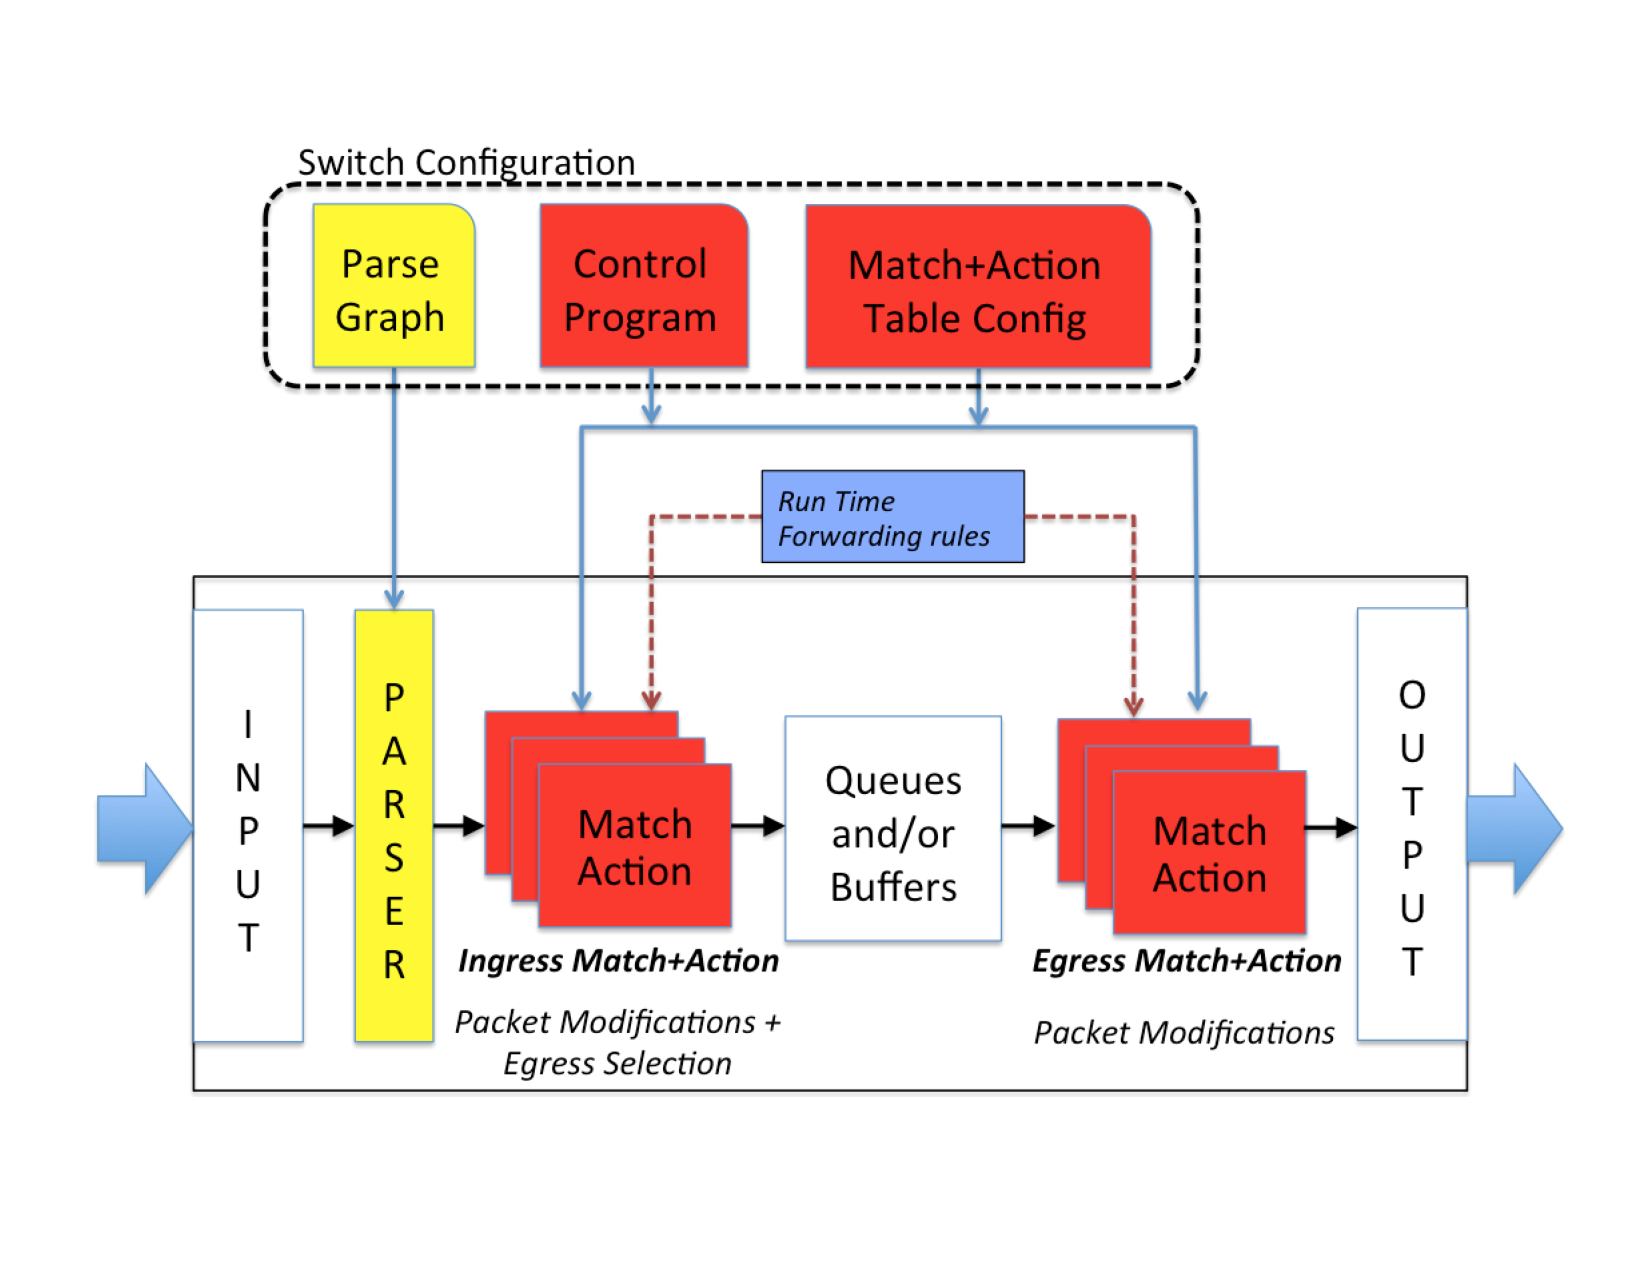
\includegraphics[width=11cm]{chapters/pic/P4DeviceModel.pdf}
    \caption{Model of P4 device (taken from \protect\cite{p4languagespec}).}
    \label{fig:originalP4DeviceModel}
\end{figure}

\subsection{Parser-Deparser Model}
\label{sec:parserDeparserModel}
Due to the disadvantage described above, we propose more general model which is based on free specification of processing part 
(simplified architecture is shown in Fig.~\ref{fig:parserDeparserArchitecture}). 
%Notice that processing part of original model consists of Ingress Match+Action, Queuing mechanism and Egress Match+Action pipeline.
Our model of network device is based on standard P4 model and it consists of three modules. 
The first module, parser, is used to break the incoming network data into individual header fields
(i.e., it has the same functionality like parser in P4 model).
The output of this module is a set of structured extracted fields and valid bits.
The valid bit is used for presence indication of extracted protocol fields in actually processed packet.
The structure of protocol fields is based on the P4's Header Format definition. 
All extracted protocol fields and valid bits are passed to the second module, process, 
which implements the general processing engine (e.g., VLAN tagging, Network Address Translation, Traffic analysis). 
This block implements the functionality of accelerated engine. It also sets a validity information for each inserted/not inserted protocol 
and filters out all unused header data (i.e., this data will not be used during packet assembling). 
Finally, the last module, deparser, is used for construction of network packet back from protocol headers and valid bits.
This approach is general enough for variety of network applications. The Parser-Deparser model is capable to accommodate the P4 device model 
because the Process part allows mapping of Ingress Match+Action, Queues and/or Buffers and Egress Match+Action to predefined general architecture. 
This work introduces possible mapping in Sec.~\ref{sec:architectureOfProcessingPipeline}.

\begin{figure}[t]
    \centering
    \includegraphics[width=\textwidth]{chapters/pic/ParserDeparserApproach}
    \caption{Parser-Deparser model.}
    \label{fig:parserDeparserArchitecture}
\end{figure} 

The VLAN tagging is a classic and common use case in many network applications. 
Tagging process consists of two main steps --- insertion of VLAN header to packet and setting of appropriate header field value of 
current Ehernet protocol.
In the case of Parser-Deparser model, the supported protocol stack is directly represented in the hardware device where each protocol
occupies one position on header and valid bus. 
Therefore, the VLAN tagging operation consists of setting of the VLAN header on header bus, setting of appropriate valid bit 
(i.e., header will be inserted) and setting of appropriate Ethernet header field value. Finally, the packet is assembled in the deparser block. 
 
The network traffic analysis is another common use case.
The analysis is based on investigation of data from extracted headers which are used 
as an input to analysis function. This function can be a general process like pattern matching, detection of malicious traffic, and so on. 
The Parser-Deparser model allows easy access to all extracted data in parallel because data are preprocessed in parser stage and put onto header
data lines. The traffic analysis algorithm is implemented in process module. This use case isn't easy to implement in standard P4 device model
because the structure and set of supported actions is predefined in P4 standard.

In this section, we proposed our Parser-Deparser model. The model can be partially generated from P4 description.
More precisely, we can generate the parser and deparser modules from the Header Format and Packet Parser definition, because both 
modules have homogeneous and general structure. Our Process block can be generated from P4, but is generic beyond what P4 describe.
In this work, we show the ability of our model. 
We use a P4 language as an input of transformation process which effectively maps the P4 source code to hardware representation.
The Parser-Deparser model is published in \cite{2016MicproP4}.

\subsection{Mapping P4 to Parser-Deparser Model}
\label{sec:architectureOfProcessingPipeline}

The following text brings details of the architecture of processing pipeline in Fig.~\ref{fig:p4PipelineArchitecture} 
(published in \cite{2016h2rc-p4}). 
The idea uses our Parser-Deparser model which was introduced in Sec.~\ref{sec:parserDeparserModel}. 
The \emph{parser} is used to break the incoming data to individual protocol header fields and payloads.
Our architecture also allows synchronization of outside metadata with parsed headers. 
The outside metadata are generated by input network buffer during receive of packet from network. 
This structure typically contains input port number and receive timestamp. The parsed headers and outside metadata are passed to the
\emph{metadata generator}. This block cooperates with parser on initialization of default metadata values.
The generated information is later used for advanced processing of parsed data in our pipeline 
(i.e., we can use metadata for controlling of functionality of processing elements).
Another output from \emph{parser} and \emph{metadata generator} is also the address of first active Match+Action processing 
element in \emph{Match+Action group}.

\begin{figure}[b]
    \centering
    
\includegraphics[scale=0.9]{chapters/pic/IPv6MorePayloads}
    \caption{The example of packet with more payloads.}
    \label{fig:IPv6MorePayloads}
\end{figure}

All outputs (parsed headers, generated metadata, address of first \emph{Match+Action group} and parsed payloads) from \emph{parser} 
and \emph{metadata generator} are passed to 
\emph{check} module. This module performs validation of the checksum field of processed packet and setting of initial values of 
control path.
Some protocols need to be checked for validity of header or payload data because there may be errors during transfer through the network
(i.e., we need to detect this situation in processed protocol and pass this information to the pipeline). 
Our architecture supports processing of protocol with such specification. 
The example of protocol with checksum field is the Transmission Control Protocol (TCP) which is defined in \cite{rfc793-TCP}.
Initial values of control path signals are generated from result of the checksum validation, start table address, incoming protocol headers
and metadata values. 
This path is used for controlling of all elements in the high-speed processing pipeline. 
Typical purpose of this path is propagation of errors, packet discarding, controlling of Match+Action element address, and so on. 
Finally, all generated control path values, parsed headers and metadata are passed to the \emph{Match+Action group} pipeline (see later). 
Parsed payloads are stored in large Payload Buffers where each buffer stores payload for one protocol. 
For example, we can receive a packet which is constructed from IPv6 header, followed by IPv6 routing header and TCP header. 
In this case, we need to extract payload from the IPv6 routing header because of its variable length 
(the length is signaled in corresponding header field). Finally, the \textit{parser} extracts payload from last available header which is the TCP.
The example of this situation is shown in Fig.~\ref{fig:IPv6MorePayloads}.

%Rotate figure with caption, angle is equal to 90°
\begin{sidewaysfigure}[p]
    
\includegraphics[height=\textheight,width=\textwidth,keepaspectratio]{chapters/pic/p4-pipeline}
    \caption{Architecture of high-speed processing pipeline.}
    \label{fig:p4PipelineArchitecture}
\end{sidewaysfigure}

The \emph{Match+Action group} is a fundamental element for running of user defined operations on parsed headers. It logically unifies
implemented functionality like VLAN tagging, network address translation, and so on. 
Each \emph{Match+Action group} contains one or more \emph{Match+Action routers} and \emph{Match+Action tables} which are 
connected to processing pipeline for implementation of required functionality.  

\emph{Match+Action table} maps incoming parsed headers and metadata to user defined actions which are performed in the same module.
Selected action in \emph{Match+Action table} depends on rules which are uploaded by configuration tool 
into \emph{Match+Action tables} at runtime. 
For example, we can upload a rule which performs network address translation for specific addresses in
given subnet, modification of parsed headers (or metedata fields), and so on. 
Each \emph{Match+Action table} also computes the address of next table or router in pipeline. 
The selection process of next table or router can be conditional (i.e., address is identified from actual header values, selected action, 
hit/miss result in match table, and so on) or unconditional (i.e., table doesn't need any additional information for computation of next address). 
Therefore, each \emph{Match+Action table} performs three operations: 
(1)~search for most suitable action based on metadata and parsed headers, (2)~identification of next table or router address and 
(3)~invocation of selected action. 

\emph{Match+Action router} is the lightweight \emph{Match+Action table} which is used for identification of next table or router address
(i.e., it doesn't contain any match or action engine). 
It is typically used for implementation of P4's \textit{if-else} selection statements. 
Generally, the selection is based on implemented logic in this module (e.g., constant, arithmetic equation, and so on).
If actual Match+Action processing element (table or router) is not addressed, all incoming data are passed through the block untouched.
We provide detailed description about \emph{Match+Action router} and \emph{Match+Action table} in Chapter~\ref{chap:matchActionProcessing}. 

All (possibly modified) headers are passed to the \emph{checksum updater} which updates protocol checksum fields.
The reason for this is that values of protocol fields may have changed in Match+Action pipeline which leads to computation of new checksum value. 
Finally, the output packet is constructed from incoming headers and payloads in \emph{deparser} block.
This block also performs possible discarding of packets (based on special signal in control path) 
because we need to remove all corresponding data from the proposed pipeline.
The last deparser's output are metadata fields from Match+Action pipeline. 
We provide this data structure to other possible algorithms and modules after the deparser. 
The example of such algorithms can be QoS, other advanced filtering, sending of deparsed packets to output port or software tool, and so on.

% Popsat zakladni vlastnosti architektury, ze je ta pipelina podobna tomu od gibba, ale ta nase umoznuje vyuzivat vice ruznych payloadu. Idealne ze je ta strutkura
% obecne definovana, cimz je ji mozne generovat. Napsat teda ze jsou dva typy sbernic (metadatova, datova a kontrolni. Ta kontrolni je staticka).
The proposed pipeline is similar to the architecture introduced by Gibb \cite{GibbPhd}. 
However, our architecture (from Fig.~\ref{fig:p4PipelineArchitecture}) is more general because it supports protocols with more payloads and we also consider 
future utilization of HLS for fast implementation of user defined actions. 
The architecture of our processing pipeline is generally defined for implementation of different network applications. 
It is based on connection of all modules by unified communication interface. The unified interface consists of:
\begin{enumerate}
    \item \textbf{Header Path} is generated from scratch because this communication line depends on set of supported protocols. 
    %The part of
    %the definition can be further specification of \textit{field list calculation} for computation of protocol checksums.
    \item \textbf{Metadata Path} can be divided into two subtypes --- static and dynamic. The static metadata are always present in 
    each implemented application.
    Structure of dynamic metadata depends on user preferences because each implemented use case requires different user defined structures.
    The text provides more details in following text.
%    Therefore, the dynamic metadata are also generated from scratch and whole bus is the combination of 
%    both (static and dynamic). The example of dynamic metadata can be a user-defined structure which holds required information for 
%    computation of network statistics, and so on.    
    \item \textbf{Control Path} is a static structure which is part of each implemented use case. 
    The main task of this interface is to control the processing in proposed pipeline. 
    Namely, it controls the selection of next \emph{Match+Action table} or \textit{Match+Action router} address,
    discarding of processed packet and propagation of possible errors. 
\end{enumerate}

\section{Mapping P4 Language to Processing Pipeline} 
\label{sec:mappingP4ToProcessingPipeline}
% Tady by to chtelo popsat jenom ve zkratce jak se casti P4 jazyka namapuji na tu predstavenou pipelinu
The following section briefly introduces the idea of mapping from P4 language constructs to our architecture. 
The P4 language is an open standard which is defined by the P4 Language Consortium in \cite{p4languagespec}. 
We briefly introduced this language in Sec.~\ref{sec:p4Language}, including basic constructs and main ideas.
As we noticed, the P4 language defines five aspects of packet processing:
\begin{enumerate}
\item \textbf{Header Format} describes protocol headers and metadata recognized by the device. 
This group also contains definition of intrinsic metadata which are part of P4 language specification (i.e., they are part of each P4 program)
\item \textbf{Packet Parser} describes the (conceptual) state machine used to traverse packet headers from 
start to end, extracting field values as it goes.
\item \textbf{Table Specification} defines how the extracted header fields are matched in possibly multiple 
lookup tables.
\item \textbf{Action Specification} defines compound actions that may be executed for packets.
\item \textbf{Control Program} puts all the above together, defining the control flow mainly among the tables.
\end{enumerate}

Tab.~\ref{tab:mappingP4ToPipeline} briefly introduces the idea for mapping of P4 program to proposed architecture. 
We will provide more details about each group in following text.

\begin{table}[h]
    \centering
    \begin{tabular}{|l|p{0.49\textwidth}|}
        \hline
        \T \textbf{Pipeline block}             & \textbf{P4 language aspects} \\
        \hline\hline
        \T Parser                              & Header Formats, Packet Parser\\  
        \T Metadata generator                  & Header Formats, Packet Parser\\  
        \T Check                               & Header Formats  \\ \hline
        \T Definition of M+A group             & Control Program \\ 
        \T M+A table                           & Table Specification, Action Specification\\ 
        \T M+A router                          & Control Program (\textit{if-else} statements)\\
        \T Ordering of M+A tables in M+A group & Control Program structure \\ \hline
        \T Checksum update                     & Header Formats\\ \hline
        \T Deparser                            & Header Formats, Packet Parser \\ \hline
        \T Metadata path                       & Header Formats \\ 
        \T Header path                         & Header Formats \\ 
         Control path                          & Static for each device:
                                            \vspace{-9pt}
                                            \begin{itemize}
                                                  \setlength{\itemsep}{0pt}
                                                  \setlength{\parskip}{0pt}
                                                \item M+A table or router address
                                                \item Error bus
                                                \item Data flow control (source/ready signals, packet drop, etc.)
                                            \end{itemize} \\
        \hline
    \end{tabular} 
    \caption{Basic mapping of P4 language aspects to high-speed pipeline blocks; M+A is abbreviation for Match+Action.}
    \label{tab:mappingP4ToPipeline}
\end{table}

\subsection{Mapping to Metadata, Header and Control Path}
This section introduces mapping of P4 program to metadata, header and control path. Each program contains specification of
supported protocol headers. We provide examples of P4 source as a reminder of this language in all corresponding sections.
The header and metadata specification has the same syntax and it looks like this:

\begin{Verbatim}[fontsize=\small]
header ethernet {
   fields {
      dst_addr  : 48; // width in bits
      src_addr  : 48;
      ethertype : 16;
   }
}
\end{Verbatim}

The proposed declaration introduces the example of Ethernet header. Each specification contains declaration of field name followed by width
in bits. P4 program typically uses header references as the lowest granularity for managing of protocol fields, selection of next used table, 
and so on. We also need to detect the availability of parsed protocol in actual processed packet. 
Therefore, each protocol header is represented by following signals:
\begin{itemize}
    \item \textbf{Data bus} for parsed protocol fields. The width of allocated bus is equal to the sum of all defined protocol fields.
    \item \textbf{Validity signal} for indication of protocol availability in actual processed packet.
\end{itemize}

The Header Format specification also supports protocols with variable protocol field length.
This situation is similar as before because protocol payloads are parsed out and moved to 
stand alone Payload Buffers and the rest of remaining header fields has the static length (known during compilation of P4 program). 

The similar situation is in the case of metadata path. The only difference is related to validity signal.
We don't need to signalize the validity of metadata path values because metadata fields are associated 
to actually processed packet and we consider them to be always valid.

The control path is used for controlling of data flow across the high-speed processing pipeline. 
It consists of following signals: (1)~identification of next table or router address, (2)~signalization of errors during packet processing 
(e.g., signalization of processing errors during execution of action in Match+Action table, and so on) and
(3)~signalization for packet flow control. The packet flow control includes signals for controlling of header and metadata 
bus transfers (source/destination ready signals) and drop control at the end of processing pipeline in deparser.

\subsection{Mapping to Parser, Metadata Generator and Check}
\label{sec:mappingToParserMetadataCheck}
This section introduces the idea for mapping of P4 program to \emph{parser} and \emph{metadata generator}. 
To achieve this task, we need to 
use two aspects of P4 language --- Header Formats and Packet Parser specification.
The first aspect, Header Formats, defines the structure of supported protocols. 
Therefore, we are able to assign extracted data vector to header fields.
We introduced details about Header Format specification in previous section.

The second aspect, Packet Parser specification, is used for the description of relations between protocol headers.
To achieve it, we can define a conceptual finite state machine which is used for extraction of incoming data.
The state for processing of Ethernet header looks like this:
\begin{Verbatim}[fontsize=\small]
header ethernet eth;
parser parse_ethernet {
   extract(eth);
   switch(eth.ethertype) {
      case 0x8100: vlan;
      case 0x9100: vlan;
      case 0x0800: ipv4;
      default : ingress;
   }
}
\end{Verbatim}

This P4's language construct was briefly introduced in Sec.~\ref{sec:p4ParserDefinition}. Simply said, the \textit{parser} 
statement defines one state of parse graph. The \textit{switch} statement defines transitions to next states (\textit{vlan} or \textit{ipv4} 
in our example) or control programs (\textit{ingress} in the code above). Graphical representation of the example is in
Fig.~\ref{fig:parseEthernetRepresentation}.
Introduced behavior needs to be implemented in processing pipeline. The architecture of
our parser is based on HFE~M2 which was introduced in \cite{hfem2}. 
%We moved the proposed work forward because we designed and developed the automatic
%generation of this parsing pipeline from P4 description. Moreover, we extended the proposed work with some internal blocks which are generated to needs 
%of analyzed protocol (i.e., these blocks are generated from scratch).
We provide more details about architecture and transformation process in Sec.~\ref{sec:parserArch}.

\begin{figure}[h]
    \centering
    
\includegraphics[scale=0.52]{chapters/pic/EthernetParseGraph.eps}
    \caption{Graphical representation of \textit{parse\_ethernet}.}
    \label{fig:parseEthernetRepresentation}
\end{figure}

The second block, \emph{metadata generator}, is used for generation of metadata field values for each processed packet. 
As we proposed before, metadata structure is inferred from Protocol Header declaration because metadata are syntactically defined in the same form. 
Initial values of metadata fields are inferred from Packet Parsed definition using the \textit{set\_metadata} statement. 
Therefore, the \emph{metadata generator} generates the initial values of all required metadata structures as described in P4 program.

Mapping to \emph{check} module is also quite straightforward and intuitive. 
The P4 program allows to define the \textit{field\_list\_calculation} statement which simply binds checksum algorithm to the list of input fields. 
This list is provided in \textit{field\_list} statement. The following example was taken from \cite{p4languagespec}:

\begin{Verbatim}[fontsize=\small]
field_list l3_hash_fields {
    ipv4.srcAddr;
    ipv4.dstAddr;
    ipv4.protocol;
    ipv4.protocol;
    tcp.sport;
    tcp.dport;
}

field_list_calculation ecmp_hash {
    input {
        l3_hash_fields;
    }
    algorithm    : crc16;
    output_width : 16;
}
\end{Verbatim}

The proposed example introduces declaration of L3 hashing, including \textit{ipv4} and \textit{tcp} protocol fields. 
The \emph{check} module setups initial values of control path signals based on result from this stage.
In the case of any error, the processed packet is marked as invalid and the next processing depends on implemented behavior of
Match+Action pipeline elements. 
The general implementation of the \emph{check} module is part of our ongoing research.
%We limit the functionality of the \emph{check} module to setting of initial control path signal values  without any checking of hash fields. 

\subsection{Mapping to Match+Action Group}
\label{sec:mappingControlToMaGroup}
This section introduces the idea for mapping of P4 program to Match+Action processing pipeline. 
The fundamental processing unit of our pipeline is \emph{Match+Action group} which logically unifies complex operations 
like ACL, packet filtering, and so on. 
Some complex programs are divided into more steps because the next step of implemented algorithm depends on the result of previous. 
The P4 language allows to define complex processing program in \textit{control program} statement. 
Each program contains one or more conditional statements (\emph{Match+Action routers}) or table calls (\emph{Match+Action tables}) 
which are connected into deep pipeline. Each \emph{Match+Action table} has three functionalities: (1)~mapping of headers and 
metadata fields to most suitable action, (2)~modification of protocol headers and metadata fields based on selected action and 
(3)~selection of next Match+Action element in processing pipeline. 
The P4 language allows to define the structure of \emph{Match+Action table} using the \textit{table} statement. 
Each P4's table statement contains two declarations: (1)~\textit{reads} statement which defines the structure of search key 
(i.e., it defines a list of used protocols/metadata fields together with matching algorithms) and 
(2)~\textit{actions} statement which defines a list of allowed actions. The simple filtering in P4 language looks like this:
\begin{Verbatim}[fontsize=\small]
// Filter table.
table filter {
    reads {
        ipv4.srcAddr : lpm;
    }
    actions {
        _permit;
    }
}

//Drop table (no read block => just run the action)
table drop {
     actions{
        _drop;
    }
}

// Filtering program
control ingress {
    // Drop all non-IPv4 traffic
    if(valid(ipv4)) {
        // Try to find the rule 
        apply(filter) {
           //Table miss  = drop packet
            miss {apply(drop);}
        }
      } else {
          // non-IPv4 traffic has been detected
          apply(drop);
      }
}
\end{Verbatim}

The proposed example introduces two tables --- \textit{filter} and \textit{drop}. The first table, \textit{filter}, defines the used protocol field 
and possible action (\textit{\_permit} in our case). The second table, \textit{drop}, defines one possible action 
(\textit{\_drop)} and no matching field. In such case, the P4 defines to use the default action. 
The \textit{control program} defines the order of Match+Action elements in the processing pipeline. 
In our case, we start with evaluation of \textit{if-else} statement which drops all non-IPv4 traffic by execution of drop table. 
The conditional statement is mapped to \emph{Match+Action router}. Each IPv4 packet is passed to the
\textit{filter} table which is followed by the \textit{drop} table in the case of table miss (in \textit{filter}).
The text provides two graphs. The Fig.~\ref{fig:grapIpv4Program} represents the graph of control program and 
Fig.~\ref{fig:matchActionIpv4Program} shows the structure of Match+Action pipeline.

\begin{figure}[h]
    \centering
    \includegraphics[scale=0.45]{chapters/pic/filter-control-program-graph}
    \caption{Graph of \textit{ingress} control program.}
    \label{fig:grapIpv4Program}
\end{figure}

The proposed example demonstrates the main idea for mapping from P4 language to pipeline of Match+Action elements. 
That is, \textit{control program} defines the \emph{Match+Action group}, all tables in a group are mapped to \emph{Match+Action tables} and all 
conditional statements are mapped to \emph{Match+Action router}.
We provide more details about the transformation of P4 program to Match+Action element pipeline in Chapter~\ref{chap:matchActionProcessing}.

\begin{figure}[h]
    \centering
    \includegraphics[scale=0.45]{chapters/pic/filter-control-program-pipeline}
    \caption{Match+Action pipeline structure of \textit{ingress} control program.}
    \label{fig:matchActionIpv4Program}
\end{figure}

\subsection{Mapping to Checksum Update and Deparser}
This section demonstrates the idea for mapping from P4 program to \emph{checksum update} and \emph{deparser} module. 
Firstly, we start with  introduction of \emph{checksum update}. The idea for mapping is similar to mapping of P4 program to \emph{check} module
(see Sec.~\ref{sec:mappingToParserMetadataCheck} for more details). 
This module also uses P4's \textit{field\_list\_calculation} statement for update of hash fields because some data may have changed 
in Match+Action processing pipeline. The general structure of this module is part of our ongoing research. 

The last module, \emph{deparser}, is the output module in proposed pipeline architecture. 
The main function of this module is to construct the output packet from incoming header fields.
\textit{Deparser}'s behavior is inferred from P4's Header Format and Packet Parser definition because deparser performs inverse operation to parsing.  
We don't discard any metadata from the processing pipeline and we transfer all fields to the output together with constructed packet. 
These metadata fields are used by other blocks after the deparser. 
We provide more details about the transformation of P4 program to \emph{deparser} in Sec.~\ref{sec:deparserArch}.

\section{Summary}
% Popsali jsme zakladni strukturu a v dalsi casti textu se budeme venovat zakladnim blokum (parser, deparser, match+action tabulky)
The chapter introduces target architectures for mapping of P4 program. 
Firstly, the text introduces not only state-of-the-art software based targets, but also more powerful hardware targets including NPUs and FPGAs.
We selected the FPGA as our target architecture because it connects the flexibility of software with parallel nature of hardware into one
compact package (i.e., the functionality of the hardware can be reprogrammed). 

Secondly, we introduced the architecture of our high-speed processing pipeline (published in \cite{2016h2rc-p4}).
The main idea of the architecture is based on the Parser-Deparser model (published in \cite{2016MicproP4}) which is flexible and suitable 
for implementation of general packet processing engine in hardware.
We demonstrate the flexibility of this approach on two common use cases --- VLAN tagging and network traffic analysis.
Finally, the last section introduces ideas for mapping of P4 language constructs
to our high-speed pipeline architecture. %, including references to following text of this thesis.

\chapter{Parser and Deparser Architecture}
\label{chap:parserDeparserArchitecture}

\begin{chapterintro}
In this chapter, we introduce the architecture of parser and deparser blocks with further details about transformation algorithm 
and generated architecture.
This chapter also introduces the experimental results for parser and deparser, including the time complexity analysis of transformation algorithms. 
%Finally, we provide the way for scaling of deparser modules to higher throughput.
\end{chapterintro}

\section{Parser Architecture}
\label{sec:parserArch}
% Sepsat zakladni architekturu HFE M2, vykopirovat z clanku z MICPRO a FCCM + jeho generovani
% Pridat algoritmus o simulaci na sbernici, vymyslet pripadny dukaz
As we noticed before, the parsing process is defined by two P4's aspects (Header Formats and Packet Parser definition). 
The following text introduces the architecture of firmware parser called HFE~M2 \cite{hfem2} 
and the transformation algorithm from a P4 description to the HDL code 
(published in \cite{2016fccm-p4-parser,2015h2rc-p4-parser,2016pesw,2016stanford-p4-demo}). 
Finally, we describe how to infer special parameters of parser which allow to reduce FPGA resources of generated engines. 

\subsection{Overview of HFE~M2 Architecture} 
\label{sec:overviewOfHfeM2}
 
The main idea of automatic generation of 100\,Gbps parsers comes from the architecture of HFE~M2 which was introduced by
Pu\v{s} et al. in \cite{hfem2}. The paper presents a block architecture of hand-written modules which 
is capable to process traffic at speed of 100\,Gbps.
However, it doesn't present any algorithm for mapping from abstract description to proposed architecture.
Therefore, we adopt the architecture of HFE~M2, identify fundamental types of blocks in Protocol Analyzer structure (see later), 
and provide transformation process from P4 language to synthesizable implementation.

The HFE~M2 architecture consists of two main block types --- Protocol Analyzers and pipelines. 
A generic interface is used for connection between the protocol
analyzers. There is an optional pipeline block between each two Protocol Analyzers.
The pipeline blocks can be individually enabled/disabled at compile time to tune the final frequency, latency and chip area.
Protocol analyzers and pipeline blocks are connected to the processing chain which represents the protocol stack of incoming 
network packet. 
An example of the HFE~M2 processing chain is shown in Fig.~\ref{fig:hfem2Arch}.

\begin{figure}[ht]
    \centering
    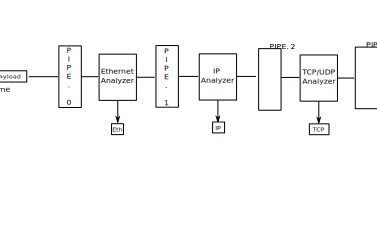
\includegraphics[width=0.95\textwidth]{chapters/pic/ParserTop}
    \caption{HFE~M2 architecture.}
    \label{fig:hfem2Arch}
\end{figure}  

Protocol analyzer uses the \textit{Generic Protocol Parser Interface} (GPPI) for connection between modules. This interface
provides the input information necessary to parse a single protocol header. That is: (1)~current packet data being
transferred at the data bus, (2)~current header offset within the packet and (3)~expected protocol to parse. 
GPPI output information includes (4)~extracted packet header field values, plus the information needed to 
parse the next protocol header: (5)~next header offset
and (6)~type of the next protocol header. More details about the GPPI can be found in \cite{hfem2}.
Brief architecture of each Protocol Analyzer block is shown in Fig.~\ref{fig:protocolArch}. 

\begin{figure}[ht]
    \centering
    \includegraphics[scale=1.25]{chapters/pic/ProtocolAnalyzer}
    \caption{Protocol analyzer architecture.}
    \label{fig:protocolArch}
\end{figure}    

Protocol analyzer architecture contains four block types: (1)~Data Extractors, (2)~Next Protocol Decoder, 
(3)~Length Generator and (4)~Adder. Data Extractors are used to extract packet data from a given offset. 
Data Extractors are configured with two parameters: \textit{Extract Length} and \textit{Extract Offset}. 
The first parameter defines the number of extracted bytes from packet data. The offset of data within the packet is computed as the sum
of current header offset (a value from input GPPI interface) and the Extract Offset parameter.
Note that Data Extractor blocks contain multiplexers which allow to extract data from any byte position. 
These multiplexers can be configured with some additional optimization parameters which  
reduce consumed FPGA resources. We describe these parameters in Sec.~\ref{sec:optimizations}.

Next Protocol Decoder is used to compute the next expected protocol. Its structure fully depends on the protocol header format.
Generally, it is a function converting some extracted packet header bytes into an internal number representing the protocol type.

Length Generator block is used to compute the length of current protocol header, so that it can be added to the Input Offset signal to obtain 
the Output Offset signal, which represents the start offset of the next protocol header.
The added offset value can be a constant or a result of an expression (see the header format specification in previous chapter).

From the perspective of parser generation, we can identify three types of blocks in the Protocol Analyzer structure 
(see Fig.~\ref{fig:protocolArch}): (1)~Static (green color), (2)~Configured (grey color), 
(3)~Fully protocol-specific (blue color). 
The static block is used in every Protocol Analyzer without any change. 
The Protocol Analyzer architecture contains only one static block, which is the adder.
This block is used to compute the next protocol offset from current Input Offset and Length Generator output. 
The second group of blocks is general enough for usage in all Protocol Analyzers, only with different parameters settings. 
The architecture contains several Data Extractor blocks which 
are instantiated (from a hand optimized template) and configured regarding to P4's Header Format specification. 
Blocks marked by blue color are entirely protocol specific, so that every Protocol Analyzer needs custom implementation of them.
This means that Protocol Decoder and Offset Generator must be uniquely generated for each Protocol Analyzer from P4's Header description.

This architecture of Protocol Analyzer is general enough for processing of most L2-L4 protocols. 
For this target block structure, we can generate, configure and connect all described blocks in automatic way from a P4 program. 
Details of this transformation process are discussed in the next section.

\subsection{Transformation from the P4 to Parser Architecture}
\label{sec:parserTransformation}

Transformation algorithm is one of the key problems addressed in this chapter.
As we note in Sec.~\ref{sec:overviewOfHfeM2}, HFE~M2 architecture consists of Protocol Analyzers and pipeline modules which are
connected to form the processing chain. 
The transformation from P4 to parser can be divided into two problems --- (1)~Generating the Protocol Analyzers and 
(2)~Generating the processing chain.
Inputs of the transformation process are P4's Header Format and \textit{Parser Graph Representation}.

We define the \textit{Parser Graph Representation} (PGR) as an acyclic oriented graph which is generated from the P4's Packet Parser definition. 
Each node (or state) represents one packet header and each transition represents the next parsed protocol header. 
Each transition is taken based on the parsed data. Condition of a transition is inferred from the P4's Packet Parser definition.
%Loop edge represents the situation when we want to support more protocols of the same type in protocol stack 
%(like VLAN or MPLS stacking, for example).
Each non-final state contains additional transition to the \textit{Unknown} state. 
This state is not explicitly described in P4 program but it is implicitly required by the parser. 
It represents the situation when no value matches the actual set of transition conditions 
(i.e., we cannot continue in parsing of next protocol header).
Each PGR node also contains a pointer to P4's Header Format definition which is needed during generation of individual Protocol Analyzers.
The PGR representation is built from a P4's Packet Parser definition.
%using the \textit{depth-first search}\,(DFS) algorithm. 
We introduce more details about this structure in the following text. 
An example of this generated representation is in Fig.~\ref{fig:parserGraph}. 
The figure doesn't show transition conditions in order to keep it well arranged.

\begin{figure}[ht]
    \centering
    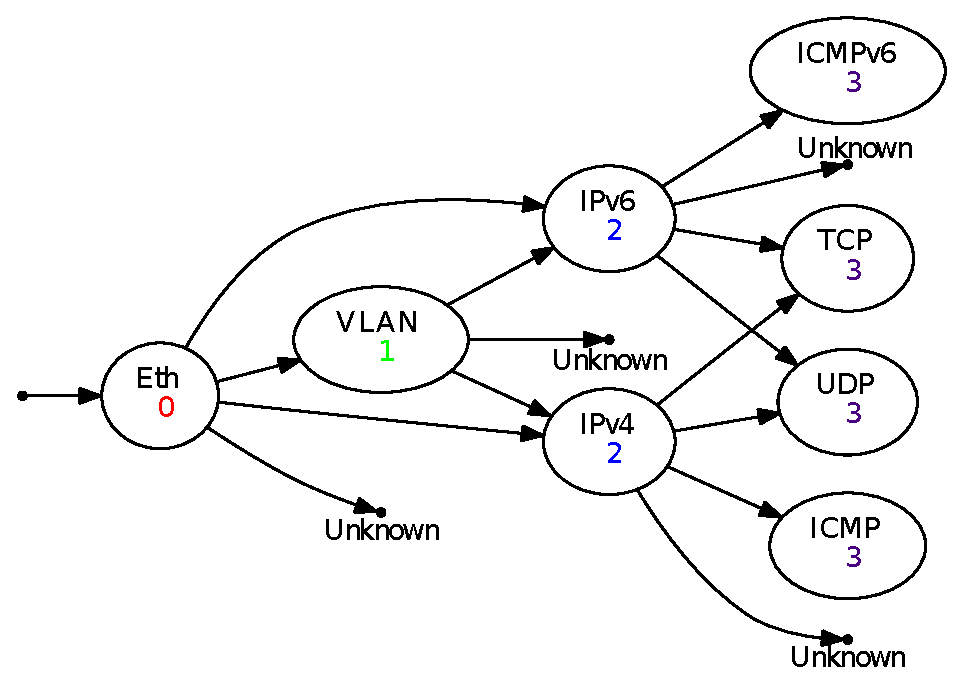
\includegraphics[scale=0.55]{chapters/pic/ParserGraph}
    \caption{Parser Graph Representation; The example supports Ethernet, VLAN, IPv4, IPv6, TCP, UDP, ICMP and ICMPv6.}
    \label{fig:parserGraph}
\end{figure}

As we note in \ref{sec:overviewOfHfeM2}, each Protocol Analyzer consists of three types of blocks (see Fig.~\ref{fig:protocolArch}). 
We now describe the generation of Protocol Analyzer block:
\begin{itemize}
\item The Length Generator block is derived directly from P4's Header Format definition. 
It can be either a constant in the case of constant length header, or a (usually simple) formula in the case of variable length header.
\item The Next Protocol Decoder is also generated from the P4's Packet Parser description. Each transition from the parser state is described
in the P4's \textit{switch} statement by the tuple, including \textit{value} and \textit{next state}. 
Therefore, we can implement Protocol Decoder by a multiplexer which selects the next protocol based on currently parsed values. 
The protocol headers that follow the currently parsed one are found in PGR during the generation.
Data Extractor blocks are parameterizable modules which are used in all Protocol Analyzers without any change, 
only by setting the parameters to match the target protocol. 
There are two parameters for each Data Extractor: Extract Length (number of bytes to be extracted) and 
Extract Offset (byte position of the extracted field, relative to the first byte of protocol header).
\item Extracted Data of Packet Analyzer can be inferred from the Header Format specification because we know the structure of protocol fields 
in the parsed protocol.
Therefore, protocol fields can be extracted from packet data using the list of protocol fields and their sizes. 
\item Adder is a static block common to all Protocol Analyzers. 
\end{itemize}

\begin{algorithm}[t]
    \caption{Recursive algorithm for identification of node levels.}
    \label{alg:longest}
    \SetAlgoLined
    \SetKwFunction{FindNodeLevels}{FindNodeLevels}
    \SetKwProg{myalg}{Function}{}{}
    \myalg{\FindNodeLevels{node, curr\_level}}{
        \KwInput{node = actual node to process}
        \KwInput{curr\_level = actual level of the node}
        \KwResult{Node with updated maximal level}
        \Begin{
            \If {node.fresh == False}
            { return\;}
            \BlankLine
            \tcc{Mark the node as not fresh and update the level}
            node.fresh = False\;
            act\_level = node.get\_level()\;
            \If{act\_level \textless curr\_level}
            { node.set\_level(curr\_level)\;} 
            \BlankLine
            \tcc{For all fresh successors, update the level and call the same function}
            node\_successors = node.get\_next\_states()\;
            \For{next\_node {\normalfont \textbf{in}} node\_successors}
            { \tcc{Don't call the node if the longest path already exists}
                \If{next\_node.get\_level() - node.get\_level() \textless 1}
                {\FindNodeLevels{next\_node,curr\_level+1}\;}
            }   
            \BlankLine
            \tcc{Mark the node as not visited}
            node.fresh = True\;
            \KwRet\;}{}}
\end{algorithm}

When generating the Next Protocol Decoder, Length Generator blocks 
and Extracted Data outputs, Data Extractors are instantiated and parametrized as needed.
Both parameters (Extract Length and Extract Offset) are directly derived from the P4 description of translated program.

Previous text introduces the automatic generation of Protocol Analyzer from P4 source code. 
The following text provides details about the automatic generation of processing chain.
The key problem is to identify a place for insertion of each Protocol Analyzer in the chain. 
Therefore, the planning algorithm has to fulfill following requirements:
\begin{enumerate}
    \item The planned structure of modules has to form a pipeline (due to the parser architecture).
    \item Protocol at the end of each transition has to be processed after the protocol at the beginning of that transition.
    \item The ordering of Protocol Analyzers has to be carefully planned because the architecture doesn't allow feedback loops.
    Planned modules have to form a totally ordered set such that it contains all possible ways through the PGR (node skipping is allowed).
    \item The ordered set can be found using the \textit{depth-first search}\,(DFS) algorithm where the output is a \textit{level} of 
    each node (i.e., the latest possible use of a protocol in pipeline).
   %The \textit{level} is used during generation of pipeline because it represents the latest possible use of a protocol in generated structure.
\end{enumerate}

\begin{algorithm}[t]
    \caption{Brief transformation algorithm from P4 to parser.}
    \SetAlgoLined
    \label{alg:transformationParserAlg}
    \SetKwFunction{TransformationToParser}{TransformationToParser} 
    \SetKwProg{myproc}{Procedure}{}{}
    \myproc{\TransformationToParser{prog}}{
        \KwInput{prog = P4 Program}
        \KwResult{VHDL code of the parser}
        \Begin{
            \tcc{1) Identify the Parser Graph Representation}
            parser\_graph = \texttt{GetParserGraphRepresentation}(\textit{prog})\;
            \BlankLine
            \tcc{2) Mark all nodes as Fresh. After that, traverse through the graph and identify level of each node}
            \texttt{MarkFresh}(\textit{parser\_graph})\;
            \texttt{FindNodeLevels}(\textit{parser\_graph.root,0})\;
            \BlankLine
            \tcc{3) Generate Protocol Analyzers and processing chain}
            \texttt{GenerateProcessingChain}(\textit{parser\_graph})\;
        }
    }
\end{algorithm}

\begin{figure}[b]
    \centering
    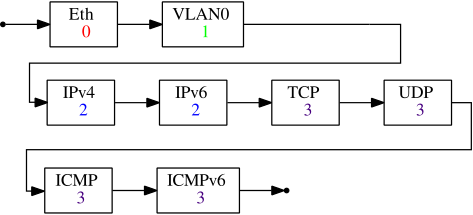
\includegraphics[scale=0.67]{chapters/pic/ParserPipeline}
    \caption{Generated processing chain; Pipeline modules are omitted for brevity.}
    \label{fig:parserPipeline}
\end{figure}

The generator of processing chain uses a PGR as an input. 
Its task is to identify the longest paths from root to each node in PGR (i.e., \textit{level} of each node). 
If we have several nodes on the same \textit{level}, we connect Protocol Analyzers in series with arbitrary ordering.
While same-\textit{level} analyzers could be connected in parallel, the serial approach allows us to keep the homogeneous structure of processing chain.
The longest paths in a PGR is found using the Alg.~\ref{alg:longest}. 
The algorithm recursively traverses and identifies node \textit{levels} in inspected graph.
The result of this algorithm is shown in Fig.~\ref{fig:parserGraph}, where each node contains a number which represents the length of the longest path 
from root. 

Finally, we introduce the Alg.~\ref{alg:transformationParserAlg} which is used for generation of complete 
parser architecture from a P4 description.
We implemented this transformation algorithm in Python language with usage of P4-HLIR \cite{p4hlir} project. 
The result of Alg.~\ref{alg:transformationParserAlg} can be seen in Fig.~\ref{fig:parserPipeline} which represents 
the processing chain generated from the PGR in Fig.~\ref{fig:parserGraph}. 
The Fig.~\ref{fig:parserPipeline} doesn't contain any pipeline modules for brevity, but the real firmware implementation contains a pipeline 
module between each two adjacent Protocol Analyzers. 
This figure also shows the situation when two or more different nodes are situated on the same level. 
Such nodes are connected in series and their relative position doesn't matter.
The only rule is to keep them together (i.e., the generator connects modules which belong to the same level in series). 


\subsection{Optimizations}
\label{sec:optimizations}

The original hand-written HFE~M2 parser supports several optimizations which save a significant amount of chip resources. 
Therefore, we have decided to support some of these optimizations in our generator as well.

The first optimization is related to Protocol Analyzer's GPPI interface. The key idea is to optimize the width of the offset bus which is used for 
signalization of protocol header start position (Input Offset and Output Offset signals). 
In another words, Input Offset and Output Offset signals are \emph{pointers} into the packet.
Since the protocol stack is being analyzed in sequential manner within the packet, the width of offset bus can increase in sequential 
manner too --- it is unnecessary to implement 
all logic (adders, etc.) at full data width, especially in early pipeline stages. 
The bus width parameter is inferred from maximal protocol header lengths
during translation. The bus width at each level is computed as a binary logarithm of the sum of all preceding protocol header lengths.
Narrower offset bus leads to smaller modules for computation of next header offset and other required values.
Therefore, we save chip resources and possibly raise the working frequency.

\begin{figure}[b]
    \centering
    
\includegraphics[scale=0.91]{chapters/pic/MuxOpt}
    \caption{The example of data extraction multiplexer: full (a), optimized (b).}
    \label{fig:muxOpt}
\end{figure}

The second optimization is related to data extraction which is performed by multiplexers within Data Extractor blocks. 
Generally, each Data Extractor is able to extract data 
from any byte position in the packet bus data word. The multiplexer is controlled by current data bus offset and offset of the 
desired field within the header. However, given the fact that the packet header may start only at certain positions on the data bus, current 
offset can contain only values with the corresponding resolution. 
This resolution is computed from P4's Header Format and Packet Parser definition. 
Using these two specifications, we identify the Offset List which contains all possible starting positions of each analyzed header in 
the processing chain. 
This knowledge is built from a protocol header length and relations between protocol headers by simulation of data transfer on data bus.
Computed lists are used for identification of required multiplexer's parameters. 
By making Data Extractors less general, we simplify the structure of each extraction multiplexer and save available chip resources. 
An example of this optimization is shown in Fig.~\ref{fig:muxOpt}. 

The multiplexer parameters can be computed from Offset List $\textbf{b}=(b_0,b_1,\dots,b_n)$ 
using the Alg.~\ref{alg:muxParamsComp} where each Offset List element represent one starting protocol offset. 
The proposed algorithm is based on observation that each offset can be expressed in the form $k*2^n + q$ where:
\begin{itemize}
    \item  $k \in {\mathbb N_0}$ represents the index of multiplexer block,
    \item  $2^n, n \in {\mathbb N_0}$ represents the size of multiplexer block,
    \item  $q, 0 \leq q < 2^n, q \in {\mathbb N_0}$ represents the offset in multiplexer block.
\end{itemize}

In other words, we want to find a common granularity for all starting offsets which are represented by a multiplexer block 
size and internal offset.

\begin{algorithm}[!b]
    \caption{Computation of multiplexer parameters.}
    \SetAlgoLined
    \label{alg:muxParamsComp}
    \KwInput{Offset List: ${\mathbf b} = (b_0, b_1, \dots , b_n), n \in {\mathbb N_0} $}
    \KwResult{Computed parameters: $n \in {\mathbb N_0}, q \in {\mathbb N_0}$}
            \BlankLine
    \tcc{Starting values (extraction from each byte position)}
    $n = 0$\;
    $q = 0$\;
    $div = 2$\;
    \BlankLine
    \While{True}{
        \tcc{Compute the reminder for each element in ${\mathbf {tmp}}$ vector}
        \For{$b_i$ \textbf{in} ${\mathbf b}$}{
            $tmp_i$ = $b_i\ mod\ div$\; 
        }
        \tcc{Check reminders in ${\mathbf {tmp}}$ vector}
        \eIf{$tmp_i == tmp_0,\ \forall tmp_i \in {\mathbf {tmp}} $} {
            \tcc{All reminders are identical. Remember the actual result and try next iteration.}
            $n = \lceil log_2(div) \rceil$\;
            $q = tmp_0$\;
            $div = 2*div$\;
        }{
            \tcc{All elements are not same. Stop the algorithm.}
            break\;
        }
    }
    \BlankLine
    \Return $n,q$
\end{algorithm}

There is also a place for optimizations of P4 program which cannot be automatically generated. 
Instead, it is required to optimize the program during design time.
The generator can then benefit from more efficient input, which results in better design in terms of latency and consumed resources. 
In this text, we introduce one such optimization 
of P4 program which leads to less Protocol Analyzer blocks being generated.
The idea is to merge protocol headers that are compatible in terms of extracted protocol header fields.
As an example, we want to extract source and destination ports of TCP and UDP protocols because their structure is similar. 
Therefore, we create a new custom protocol header which describes export of interesting fields.  
We don't have to worry about incomplete protocol header specification because our replaced protocol headers are 
leaves of the PGR (see Fig.~\ref{fig:parserGraph}), so that there is no further processing after this merged header.
We define the new protocol header like this:
\begin{Verbatim}[fontsize=\small]
header tcp_udp_t {
   fields {
      src_port : 16; // width in bits
      dst_port : 16;
   }
}
\end{Verbatim}

\subsection{Time Complexity of the Transformation}
\label{sec:parserTimeComplexity}

Time complexity of the proposed transformation Alg.~\ref{alg:transformationParserAlg} consists of following components (consider situation
without computation of multiplexer parameters):
\begin{enumerate}
    \item \texttt{GetParserGraphRepresentation}'s time complexity is equal to $\mathcal{O}(V+E)$ (DFS algorithm), where $V$ is the number of nodes and 
$E$ is the number of edges. Our transformation algorithm requires PGR with no cycles.
In general, maximal number of edges in acyclic graph is equal to $\frac{n}{2}*(n-1)$ where $n$ is the number of Protocol Analyzers 
(i.e., nodes of our graph). Total time complexity of DFS is $\mathcal{O}(n+\frac{n}{2}*(n-1)) \sim \mathcal{O}(n^2)$.
    \item \texttt{FindLongestPaths}'s time complexity is equal to $\mathcal{O}(n^2)$ (DFS algorithm), where $n$ is the number of Protocol Analyzers.
    \item \texttt{MarkFresh}'s time complexity is equal to $\mathcal{O}(n)$, where $n$ is a number of protocols (i.e., nodes of PGR).
    \item \texttt{GenerateProcessingChain}'s time complexity is equal to $\mathcal{O}(n)$ because generated processing chain contains $n$ 
    Protocol Analyzers. 
\end{enumerate}

Total time complexity of the transformation (without computation of multiplexer parameters) is 
$\mathcal{O}(n^2)+\mathcal{O}(n^2)+\mathcal{O}(n)+\mathcal{O}(n)=\mathcal{O}(2*n^2)+\mathcal{O}(2*n) \sim \mathcal{O}(n^2)$.

The list of protocol offsets is constructed using the DFS algorithm. Therefore, the time complexity is $\mathcal{O}(\frac{n}{2}*(n-1))$
where $n$ is the number of Protocol Analyzers. Notice that the length of Protocol Analyzers's offset list depends on complexity of PGR.

Computation of multiplexer parameters cannot use more than $\mathcal{O}(log_2(\max({\mathbf b})))$ iterations 
(i.e., the number of binary digits of maximal element in the vector) where the algorithm
requires $\mathcal{O}(\text{len}(\mathbf{b}))$ time for initialization of $tmp$ vector and $\mathcal{O}(\text{len}(\mathbf b))$ for check of
all reminders in $tmp$ vector. The total time complexity of the algorithm is 
$\mathcal{O}(2*\text{len}(\mathbf b)*log_2(\max({\mathbf b}))) = 
\mathcal{O}(\text{len}(\mathbf b)*log_2(\max({\mathbf b})^2))$ where
$\mathbf b$ is a merged list of protocol offsets of all Protocol Analyzers.

\section{Deparser Architecture}
\label{sec:deparserArch}
% Sepsat zakladni architekturu deparseru, ta se muze vzit z MICPRO
% Pridat zakladni info o propustnosti (udelat analyzu)
The deparser module is used to assemble packets back from modified protocol headers. 
The architecture of our deparser module (published in \cite{2016pesw,2016h2rc-p4,2016MicproP4}) is similar to HFE~M2 \cite{hfem2}. 
It consists of two modules --- Protocol Appenders and pipelines. 
Protocol Appender effectively inserts a protocol header before payload (i.e., it merges protocol header and payload). 
There is an optional pipeline block between each two Protocol Appenders. This pipeline block has the same 
reason as in the case of parser pipelines. They are also used for tuning of final frequency, latency and chip area. All modules
are connected to the processing chain which represents the supported protocol stack. 
Brief architecture is 
shown in Fig.~\ref{fig:deparserArch}. The figure also introduces the main idea of deparser's architecture --- all modules are connected
in reverse order (from upper protocol layers to lower protocol layers), where each Protocol Appender inserts the header at zero offset. 
Generally, there are two approaches for stacking of appending units --- botom-to-up and up-to-bottom. 

\begin{figure}[ht]
    \centering
    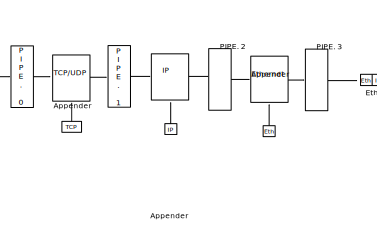
\includegraphics[width=0.95\textwidth]{chapters/pic/DeparserTop}
    \caption{Deparser architecture.}
    \label{fig:deparserArch}
\end{figure}

The bottom-to-up approach is similar to the solution of parser (i.e., insertion from lower protocol layers to upper protocol layers). 
This approach is natural for the implementation in a software program which typically fills the packet memory in sequential manner.
However, this is not suitable for hardware implementation because each Protocol Appender would have to support multiple \emph{insertion offsets} 
(the set of supported insertion offsets depends on previously inserted headers). 
This leads to more complex shifting logic which consumes more FPGA resources.

The up-to-bottom approach makes the assembling process easier because 
the appended header is inserted always at the beginning of the packet (i.e., at zero offset).
To make that possible, the incoming data of unfinished packets must be shifted to make space for the new header.
The incoming data are fixed to zero offset. 
Therefore, the shifting logic is insensitive to previous Protocol Appenders and the complexity of shifting logic depends only on the current protocol.

The Protocol Appender uses a generic interface for connection between modules. This interface provides the input information 
necessary to assemble a single protocol header. That is: (1)~current protocol header fields to be inserted, (2)~current (unfinished) packet 
to insert the header into and  (3)~header insertion vector where each Protocol Appender observes one bit position. 
This observed bit enables or disables the header insertion. 
The output information includes (4)~merged data and (5)~unmodified header insertion vector.
Notice that incoming unfinished packet always starts on the first byte of data bus.

\begin{figure}[ht]
    \centering
    \includegraphics[scale=1.27]{chapters/pic/ProtocolAppender}
    \caption{Protocol Appender architecture.}
    \label{fig:protocolAppender}
\end{figure}

Architecture of Protocol Appender contains three block types: (1)~Data Width Transform, (2)~Header Merger and (3)~Enable logic.
The Data Width Transform unit is used to transform the header from its native data width (w1), given by the sum of its fields, to the width of 
the main data pipeline (w2).
This transformation leads to a simpler data merging process. The Enable logic is a simple detector which observes predefined 
bit position in header insertion vector. The observed bit enables or disables the header insertion. 
The width of this input vector equals to the number of used Protocol Appenders in the processing chain. 

The Header Merger consumes three inputs --- transformed header data, payload and enable signal. 
It is divided into three
sub-blocks. The first, Data Shifter, is used to make a free space in the incoming unfinished packet data.
It moves the data behind the free space where the current packet header is to be inserted
in Data merger sub-block. The Data merger sub-block implements an effective merging logic where both inputs (header and payload) 
are masked by logical \textit{and} operation and merged by logical \textit{or} operation. 
The whole process of merging is controlled by the Finite State Machine (FSM) which controls the logical operations. If no header is 
inserted in actual Protocol Appender stage, the FSM disables header interface (i.e., \textit{and} operation with data and zero vector) and
the payload is transferred unchanged (i.e., logical \textit{or} between zero vector and incoming payload is performed).
 
There is also a possible optimization which can be inferred from the property of incoming protocol. All protocols can be
divided into two groups --- protocols with static and dynamic header length. In the first group, we have to support two shifting
offsets --- zero offset (i.e., no change of payload structure) and static offset (i.e., offset of shifted payload by a constant). 
This kind of offset can be computed with equation \ref{eq:offset} where $l$ is the length of inserted header in bytes and $w$ 
is the width of payload bus in bytes. In other words: payload is shifted to the next available byte position behind the inserted header. 
The proposed equation can be used if inserted header doesn't occupy the whole output bus width 
(the result of the equation \ref{eq:offset} differs from zero). 
If header occupies the output bus (the result equals to zero), 
we have to move the payload insertion to the next bus cycle with zero offset value 
(i.e., we don't need to modify the offset of incoming payload).
The example of header insertion is demonstrated in Fig.~\ref{fig:protocol-appender-princip}.

\begin{equation}
\textrm{offset} \equiv (l+1) \;(\bmod\; w)
\label{eq:offset}
\end{equation}

The case with dynamic protocol length is more complex, because we need to support more shifting offsets. The reason
for this is straightforward --- we don't know the exact length of the protocol header during the compile time. 
Therefore, we have to support more complex shifting logic based on granularity of inserted protocol.
The shifting multiplexer can be also optimized in similar way like data extraction multiplexers in parser.

\begin{figure}[ht]
    \centering
    \includegraphics[scale=0.45]{chapters/pic/ProtocolAppenderPrincip}
    \caption{The example of header insertion in Protocol Appender.}
    \label{fig:protocol-appender-princip}
\end{figure}

\subsection{Transformation from the P4 to Deparser Architecture}
\label{sec:deparserTransfAlg}

The transformation algorithm from P4 to deparser architecture is quite similar to generation of parser. We can reuse
the PGR and \textit{depth-first-search}\,(DFS) algorithm for identification of node levels. 
After the identification, we reverse the order of Protocol Appender modules.
The transformation algorithm can be described using the Alg.~\ref{alg:transformationDeparserAlg}

\begin{algorithm}[ht]
    \caption{Brief transformation algorithm from P4 to deparser.}
    \SetAlgoLined
    \label{alg:transformationDeparserAlg}
    \SetKwFunction{TransformationToDeparser}{TransformationToDeparser} 
    \SetKwProg{myproc}{Procedure}{}{}
    \myproc{\TransformationToDeparser{prog}}{
    \KwInput{prog = P4 Program}
    \KwResult{VHDL code of the deparser}
        \Begin{
            \tcc{1) Identify the Parser Graph Representation}
            parser\_graph = \texttt{GetParserGraphRepresentation}(\textit{prog})\;
            \BlankLine
            \tcc{2) Mark all nodes as Fresh. After that, traverse through the graph and identify level of each node}
            \texttt{MarkFresh}(\textit{parser\_graph})\;
            \texttt{FindNodeLevels}(\textit{parser\_graph.root,0})\;
            \BlankLine
            \tcc{3) Reverse the order of PGR nodes and generate the processing chain}
            deparser\_graph = \texttt{ReverseNodeLevels}(\textit{parser\_graph})\;
            \texttt{GenerateDeparsingChain}(\textit{deparser\_graph})\;
        }
    }
\end{algorithm}

The result of the proposed algorithm is a processing chain similar to the example in Fig.~\ref{fig:parserPipeline}.
The only difference is the reversed order of all modules. 

\subsection{Time Complexity of the Transformation}
The time complexity of the Alg.~\ref{alg:transformationDeparserAlg} is similar to the Alg.~\ref{alg:transformationParserAlg}.
However, there are two important differences. The first difference is related to \texttt{GenerateDeparsingChain}. 
This function contains computation of multiplexer parameters for appending logic. The logic needs to support just offsets of appended protocol. 
Therefore, the number of supported offsets is typically smaller than the list of supported offsets in the last Protocol Analyzer of 
more complex PGR. 
The second difference is related to the \texttt{ReverseNodeLevels}. 
This function is used for generation of deparser's structure in $\mathcal{O}(n)$ time where $n$ is the number of Protocol Appenders. 
Therefore, the time complexity of the Alg.~\ref{alg:transformationDeparserAlg} is
$\mathcal{O}(n^2)+\mathcal{O}(n^2)+\mathcal{O}(n)+\mathcal{O}(n)+\mathcal{O}(n)=\mathcal{O}(2*n^2)+\mathcal{O}(3*n) \sim \mathcal{O}(n^2)$.

\section{Parser-Deparser Experiments}
% Sepsat tady analyzu jaka bude minimalni mozna propustnost, vyjde ze to neda maximum 100 Giga, ale
% mame obecne reseni, ktere se da pouzit i v jinych resenich (porad je to obecne). Vysledky mereni
% v FPGA.
In this section, we introduce results for parser and deparser because both modules are usable standalone.
We have tested properties of generated parsers with two different protocol stacks:
\begin{itemize}
    \item \textbf{simple L2} - Ethernet, IPv4/IPv6 (with 2$\times$extension headers), TCP/UDP, \\ ICMP/ICMPv6
    \item \textbf{full} - Ethernet, 2$\times$VLAN, 2$\times$MPLS, IPv4/IPv6 (with 2$\times$extension headers), \\ TCP/UDP, ICMP/ICMPv6
\end{itemize}

For each protocol stack, we compare the manually optimized HFE~M2 parser and the generated parser with all optimizations enabled. The 
deparser isn't compared to a hand optimized version because this architecture was tailored to needs of 
automatic generation and there is no other hardware based deparser available.
All tested designs implement both engines without any additional logic like outputs FIFOs for parsed data, cleanup logic, etc. 
We choose this approach because the additional logic typically depends on the character of implemented application. 
We use the Slice Logic (number of used LUTs plus FlipFlops) as a metric of resource utilization because these parts are the most utilized in 
most FPGA designs.

We provide results after synthesis for the Xilinx Virtex-7 XCVH580T FPGA using the Xilinx Vivado 2015.1 design tool. 
All designs were synthesized with different settings of data width and presence of pipeline modules. 
These settings, together with the resulting frequency, latency and resource usage, generate a large space of
possible solutions for each P4 program. 
These solutions were searched for Pareto set which allows us to pick the best-fitting solution for an application.

\subsection{Results for the Parser}
\label{sec:exprParser}

In each \textbf{hand optimized} design test case, we
use two different data widths: 256 and 512 bits. For each data width, every possible placement of pipelines was tested: $2^{9}$ possible combinations 
in the case of the full protocol stack and $2^{5}$ combinations in the case of simple L2 protocol stack (because there are 9 and 5 configurable pipeline stages). 

In each \textbf{generated} parser test case, we use two different data widths: 256 and 512 bits. 
For each simple L2 parser, every possible placement of pipelines was tested: $2^{10}$ possible combinations. 
In the case of full parser, there are $2^{14}$ different configurations. We have randomly selected 20\% of all possible solutions.
This approach allows us to briefly inspect properties of generated processing chain in a reasonable compile time.

We provide two graphs with Pareto sets: one showing Pareto sets optimized for throughput and chip area without any regard to latency, 
and second optimized for throughput and latency without any regard to FPGA resources. 
Before the graphs, we introduce results for optimizations which are described in 
Sec.~\ref{sec:optimizations} because they have an influence on latency and used resources. We define the following notation:
\begin{itemize}
    \item \textbf{No optimizations (O0)} - no optimizations are used.
    \item \textbf{Offset optimization (O1)} - optimization of the offset width.
    \item \textbf{Offset + multiplexer optimization (O2)} - offset and multiplexer optimizations.
    \item \textbf{Optimized P4 program (O3)} - O0 version with effectively written P4 program (manual optimization).
    \item \textbf{All optimizations (O4)} - all proposed optimizations are used.
\end{itemize}

Resource utilization (values in parentheses represent the percentual usage of available FPGA's resources) and latency for parsers 
generated with different optimizations are shown in Tab.~\ref{tab:optMethod}. The table shows the influence of proposed optimizations on
similar hardware configurations with throughput around 100\,Gbps. 

\begin{table}[ht]
    \centering
    \begin{tabular}{|c||c|c|c|c|c|}
        % Header
        \hline
        \T{\textbf{Opt.}} &
        \T{\textbf{Pipes}} &
        \T{\textbf{Latency [ns]}}   & 
        \T{\textbf{Thr. [Gbps]}}  & 
        \T{\textbf{Slice LUT [-]}} & 
        \T{\textbf{Slice Reg [-]}} \\
        \hline\hline
            O0  &    8      &        39.8        &   102.7     &   25335\,(6.98\%)          &   5055\,(0.69\%)           \\ 
            O1  &    14     &        75.3        &   101.9     &   21477\,(5.91\%)          &   8930\,(1.23\%)           \\ 
            O2  &    8      &        46.1        &   100.0     &   10103\,(2.78\%)          &   5537\,(0.76\%)           \\
            O3  &    9      &       44.5         &   115.1     &   14270\,(3.93\%)          &   5427\,(0.74\%)           \\  
            O4  &    7      &       40.7         &   100.7     &   8314\,(2.29\%)           &   4795\,(0.66\%)           \\
        \hline
    \end{tabular}
    \caption{Comparison of different optimization methods with resource consumption for the Xilinx Virtex-7 XCVH580T FPGA.}
    \label{tab:optMethod}
\end{table} 

For all the following results we use O2 optimization, since O3 and O4 require manual modifications to the original P4 program.
We consider this kind of optimization to be highly non-standard.

For comparison of the achieved Pareto set results for different protocol stacks, we provide graphs in Fig.~\ref{fig:hfeParetoLut} 
(throughput and FPGA resources) and Fig.~\ref{fig:hfeParetoLat} (throughput and latency).
The Pareto sets show the best achievable solutions for our parsers. From these figures, we can see that supported protocol stack can significantly 
change parameters of the parser in terms of FPGA resources and latency. 
We can also see that P4 based parsers are approximately two times worse than hand-written parsers in terms of latency and consumed resources. 

\begin{figure}[b]
    \centering
    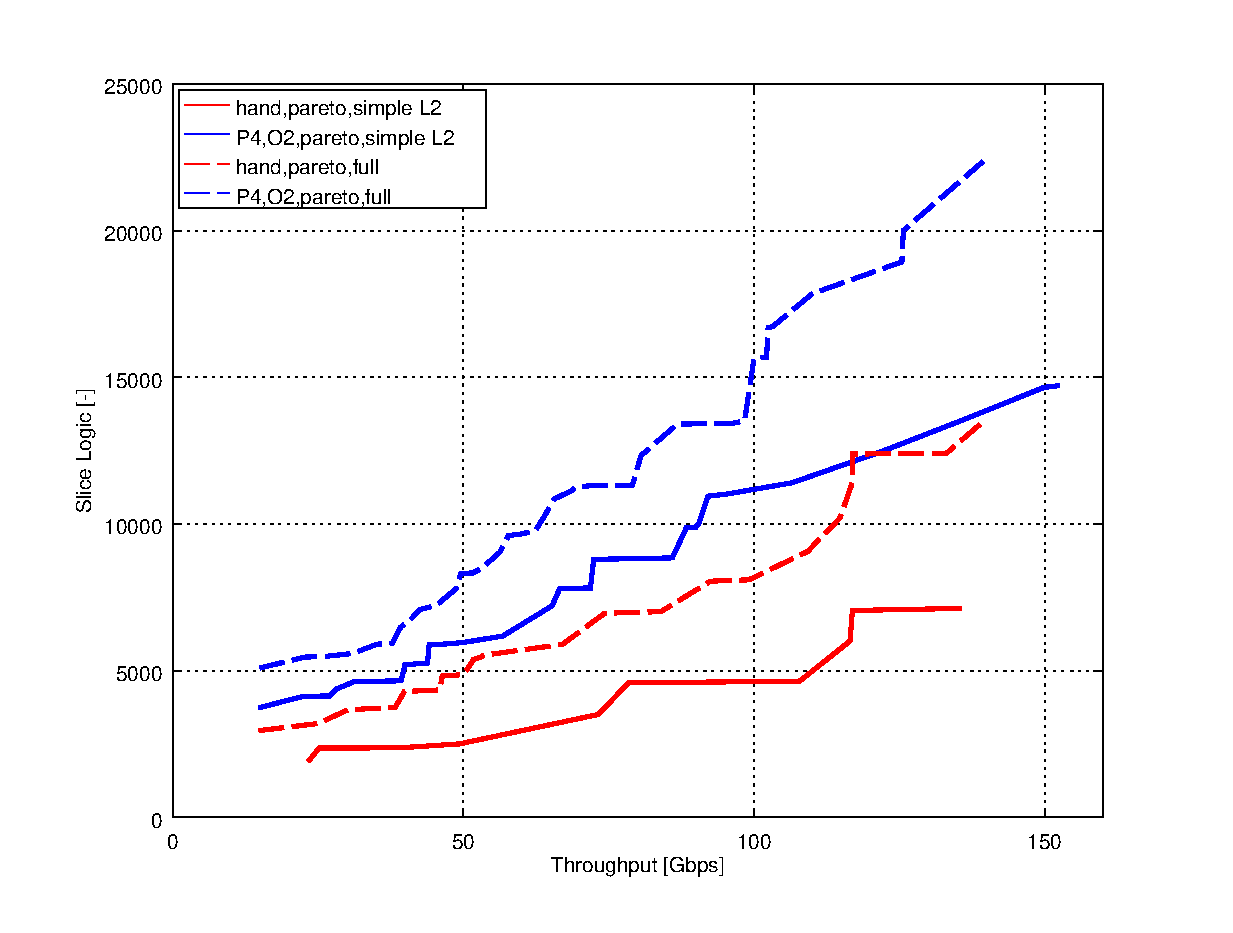
\includegraphics[scale=0.61]{chapters/pic/graphs/hfe/1_thrslice_logic_pareto}
    \caption{Parser - Comparison of the FPGA resource utilization versus throughput Pareto sets for the tested protocol stacks.}
    \label{fig:hfeParetoLut}
\end{figure}

\begin{figure}
    \centering
    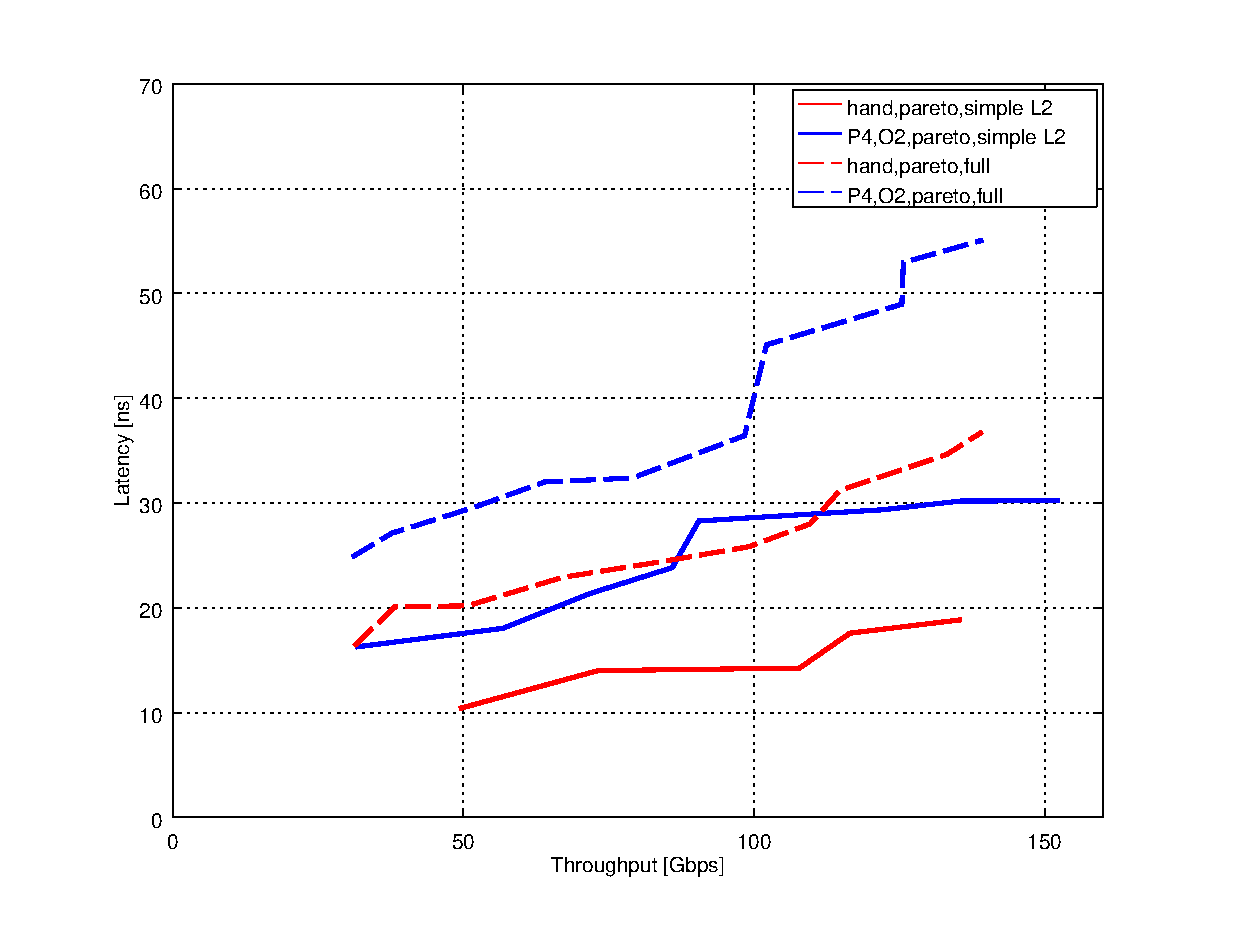
\includegraphics[scale=0.61]{chapters/pic/graphs/hfe/2_thrlat_pareto}
    \caption{Parser - Comparison of the latency versus throughput Pareto sets for the tested protocol stacks.}
    \label{fig:hfeParetoLat}
\end{figure}

\begin{figure}
    \centering
    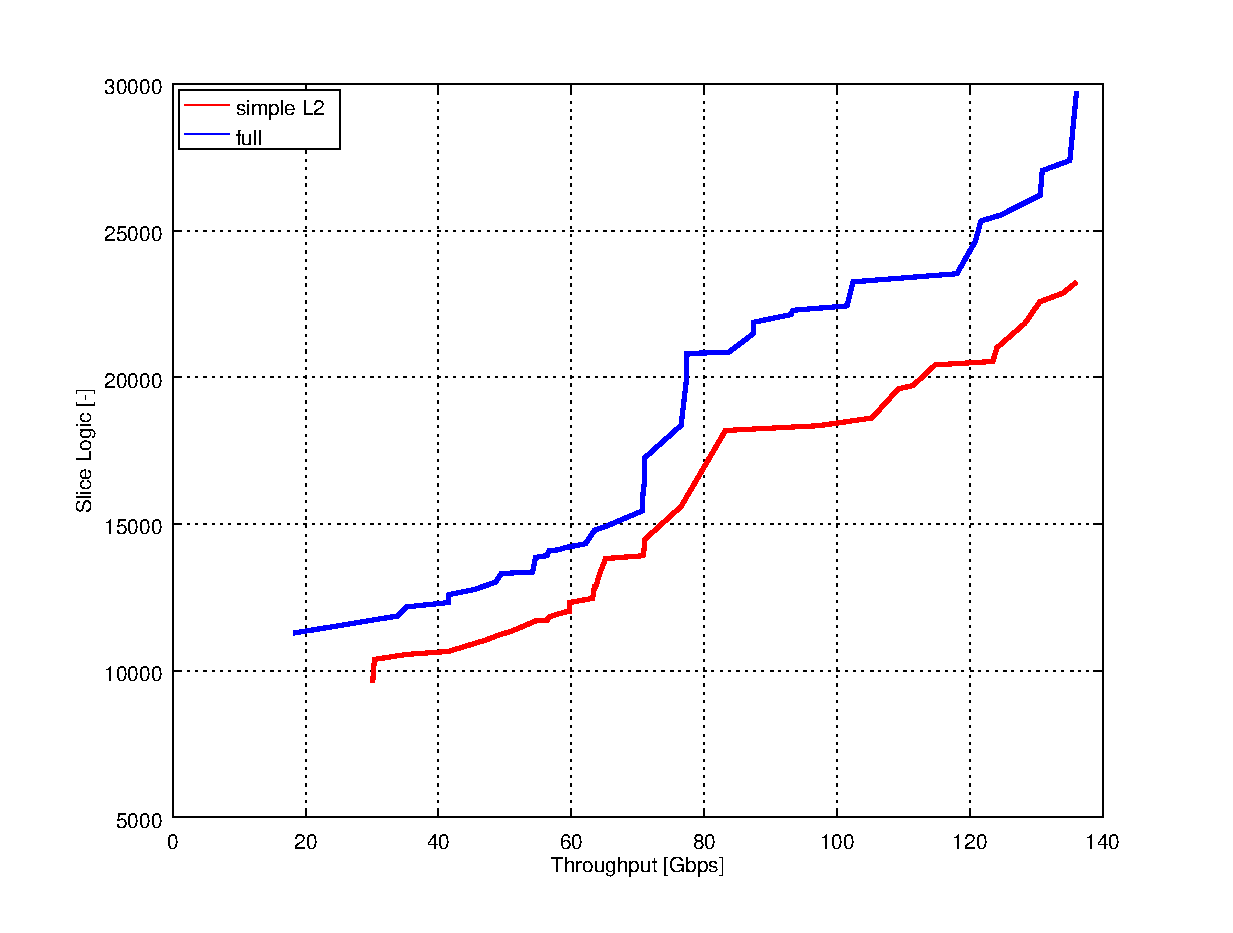
\includegraphics[scale=0.61]{chapters/pic/graphs/deparser/1_thr_slice_logic_pareto}
    \caption{Deparser - Comparison of the FPGA resource utilization versus throughput Pareto sets for the tested protocol stacks.}
    \label{fig:deparserParetoLut}
\end{figure}

\begin{figure}
    \centering
    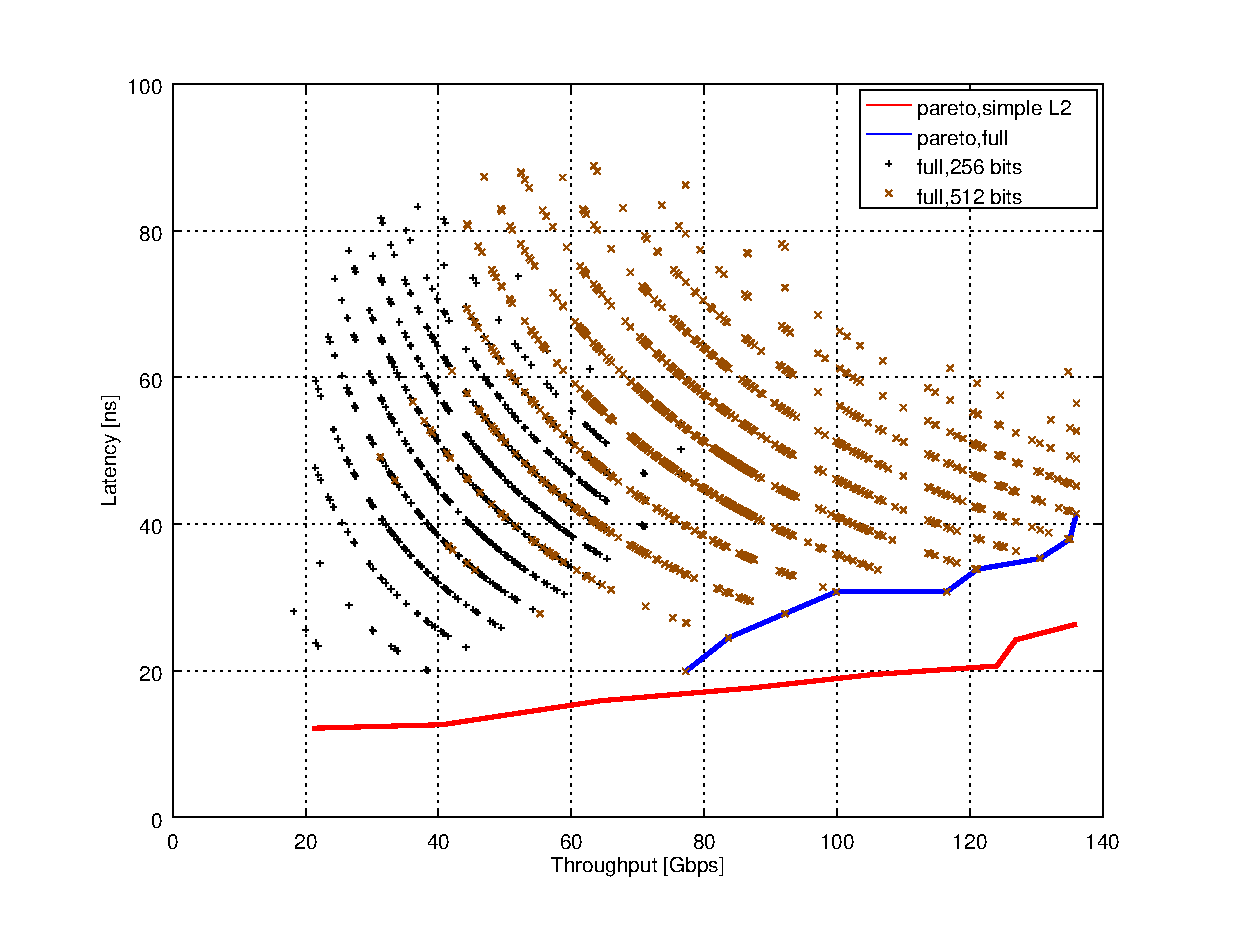
\includegraphics[scale=0.61]{chapters/pic/graphs/deparser/3_thr_latency_deparser.eps}
    \caption{Deparser - Comparison of the latency versus throughput Pareto sets for the tested protocol stacks.}
    \label{fig:deparserParetoLatency}
\end{figure}

\subsection{Results for Deparser}
\label{sec:exprDeparser}

This section introduces results for the deparser module which is used for composition of output packet. We provide graph in
Fig.~\ref{fig:deparserParetoLut} which introduces Pareto sets optimized for throughput and chip area. The graph also 
shows that consumed resources are higher compared to parser with the same throughput. The reason for this is the fact that
each Protocol Appender contains payload shifting logic which consumes more resources than Data Extractor units in parser.
The second graph, Fig.~\ref{fig:deparserParetoLatency}, introduces Pareto sets optimized for throughput and latency. 

The experiment data were measured in the same way like experiments for \textbf{generated} parsers test cases. 
The generated test cases were chosen because we don't have any hand-optimized version of deparser which supports given protocol stacks 
(the architecture of deparser was developed with respect to automatic generation of target architecture). 
Pareto set for latency of full protocol stack starts approximately from 78\,Gbps (see Fig.~\ref{fig:deparserParetoLatency}). 
We provide additional information for illustration of all measured data where each point represents a result for a specific 
configuration of deparser's pipeline.

\subsection{Parser-Deparser Throughput}
\label{sec:exprParserDeparserThroughput}
This section introduces the throughput analysis of Parser-Deparser blocks for the full protocol stack (see Sec.~\ref{sec:exprParser} for details). 
Two use cases will be introduced --- No modification and VLAN tagging.
The first, No modification, represents the raw throughput of both blocks where no changes are performed in parsed headers. 
The second, VLAN tagging, represents the throughput of the generated device during insertion of VLAN header. 
Both engines were generated and synthesized for COMBO-100G card \cite{combo-100g} using the Xilinx Vivado 2015.4 design tool. 
The proposed device is equipped with the Xilinx Virtex-7 XCVH580T FPGA and is capable to process traffic up to 100\,Gbps. All implemented
designs were running at speed of 220\,MHz. We provide two graphs: one showing the percentage throughput of 100\,Gbps Ethernet line and 
second showing the number of mega packets per second (Mpps).

\begin{figure}
    \centering
    \begin{subfigure}[b]{0.8\textwidth}
        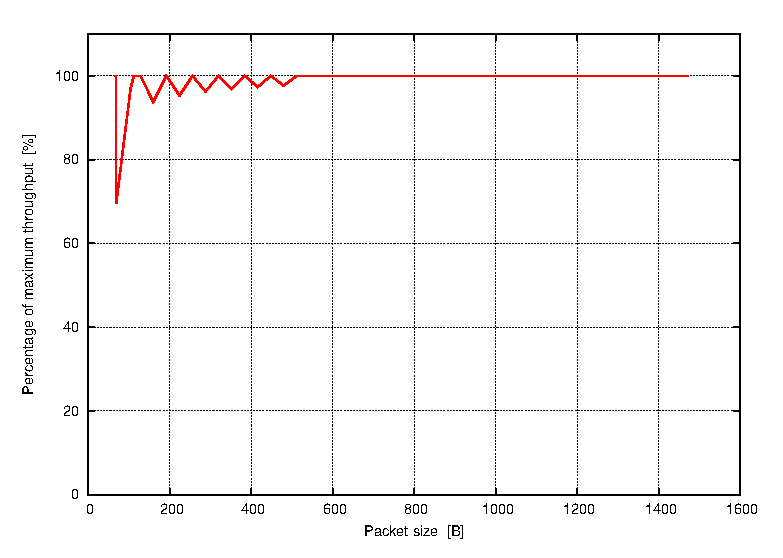
\includegraphics[width=\textwidth]{chapters/pic/graphs/parser-deparser/full-plain/throughput.eps}
        \caption{Percentage of maximum throughput.}
        \label{fig:bitThroughputPlain}
    \end{subfigure}
    ~
    \begin{subfigure}[b]{0.8\textwidth}
        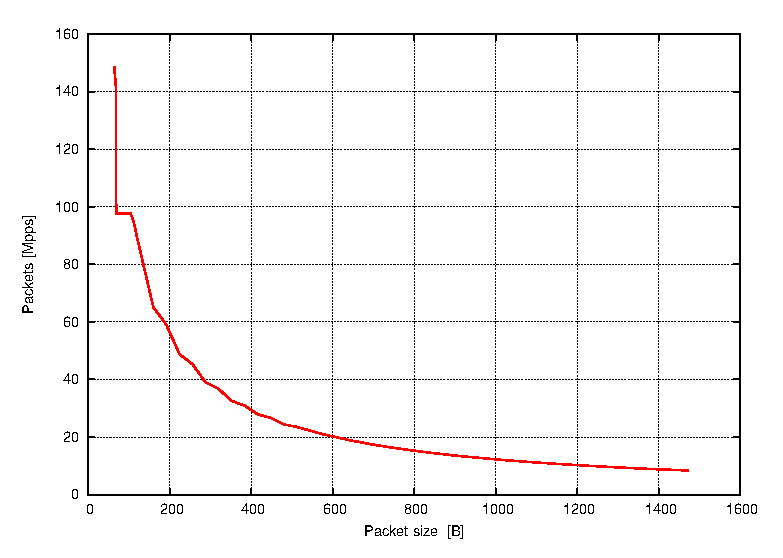
\includegraphics[width=\textwidth]{chapters/pic/graphs/parser-deparser/full-plain/mpps-throughput.eps}
        \caption{Packet rate.}
        \label{fig:packetThroughputPlain}
    \end{subfigure}
    
    \caption{Throughput of generated Parser-Deparser device for the No modification use case.}
    \label{fig:noModThroughput}
\end{figure}

\begin{figure}
    \centering
    \begin{subfigure}[b]{0.8\textwidth}
        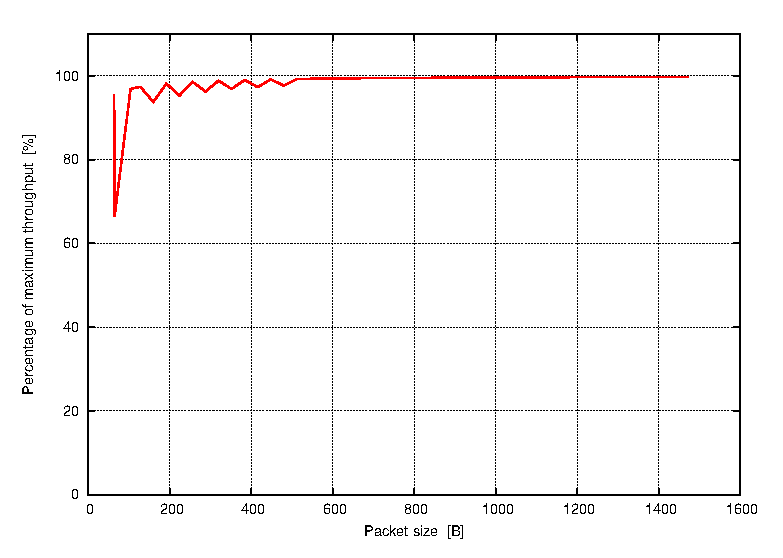
\includegraphics[width=\textwidth]{chapters/pic/graphs/parser-deparser/full-vlan/throughput.eps}
        \caption{Percentage of maximum throughput.}
        \label{fig:bitThroughputVlan}
    \end{subfigure}
    ~
    \begin{subfigure}[b]{0.8\textwidth}
        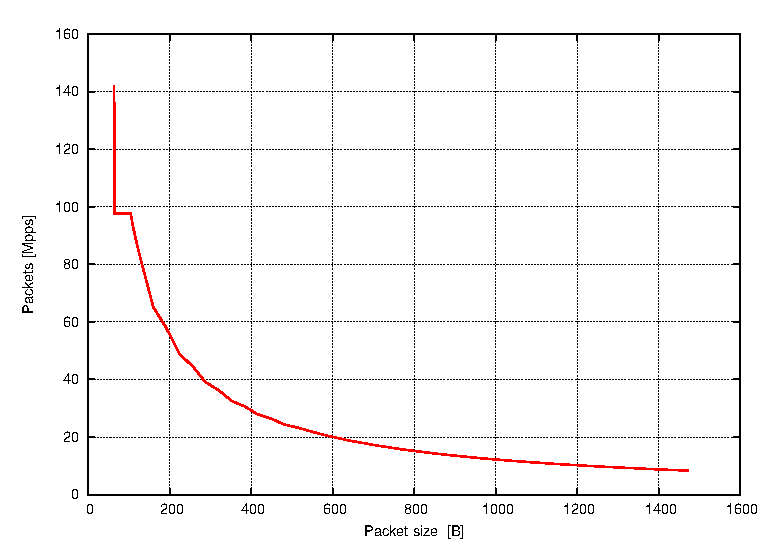
\includegraphics[width=\textwidth]{chapters/pic/graphs/parser-deparser/full-vlan/mpps-throughput.eps}
        \caption{Packet rate.}
        \label{fig:packetThroughputVlan}
    \end{subfigure}
    
    \caption{Throughput of generated Parser-Deparser device for the VLAN tagging use case.}
    \label{fig:vlanThroughput}
\end{figure}

The Fig.~\ref{fig:noModThroughput} introduces results of raw throughput (no header modification or insertion was performed). 
We see that generated device is capable to process data at speed of 100\,Gbps. 
However, there are some packet lengths where the throughput falls below 100\,Gbps. 
This decrease of throughput is caused by ineffective usage of available output data bus in deparser.
The most complicated situations occurs on short Ethernet frames. 
We demonstrate this problem on 512 bits wide data bus during transfer of 69 bytes (start of the frame is aligned to the first byte of data bus). 
In this situation, we need to use two bus cycles during which we transfer 69 bytes of Ethernet frame. 
Unfortunately, we are wasting available capacity (i.e., we use 69 bytes from 128 bytes available). 
The case gets less significant with longer Ethernet frames because the data bus is used for longer time and we need to reach smaller packet rate. 
Therefore, minimal throughput of aligned transfer on given packet length can be roughly computed using the equation \ref{eq:thrEq} 
where $dw$ is width of data bus, $freq$ is working frequency, $pkt\_len$ is length of a packet in bytes and $min\_cycles$ is the required 
number of bus cycles for transfer of the packet.

The situation for the VLAN tagging use case is introduced in Fig.~\ref{fig:vlanThroughput}. 
There is one additional source of decrease of throughput: inserting the VLAN tag makes the output packet 4 bytes longer.
Therefore, the rate of packets decreases which leads smaller overall throughput (when measured at input).   

\begin{flalign}
\label{eq:thrEq}
 min\_throughput =& (dw*freq)*\frac{pkt\_len*8}{min\_cycles*dw} & \\ \nonumber 
 =& freq*\frac{pkt\_len*8}{min\_cycles} &  [bps]  \\
\nonumber \\
min\_cycles =& \ceil{\frac{pkt\_len*8}{dw}} &  [-] \nonumber
\end{flalign}

The ineffective transfer can be solved by following idea --- we need to generate and merge more network streams to one output 
line (we need to prepare required number of packets and merge them on output bus). 
Such solution will be capable to eliminate ineffective data transfer in deparser and reach the full output packet rate.
Overview of this solution is shown in Fig.~\ref{fig:deparserInefElim}. 
We presented the approach for effective merging of network streams (architecture of \textit{Merge} block) in \cite{2014binder}.

\begin{figure}[h]
    \centering
    
\includegraphics[scale=0.68]{chapters/pic/deparsers-binder}
    \caption{Idea for elimination of ineffective data transfer in deparser.}
    \label{fig:deparserInefElim}
\end{figure}

\section{Summary}
% Napsat, ze jsme prosli zakladni vstupni a vystupni bloky a ze oba se daji automaticky generovat a ze 
% mohou pracovat na 100 Gbsp
We addressed three problems in this chapter --- automatic generation of parser, automatic generation of deparser and 
possible way for scaling of deparser to higher throughput.
The automatic generation of parsers uses the HFE~M2 architecture which was introduced in \cite{hfem2} 
(see Sec.~\ref{sec:parserArch} for more details).
We introduced an effective and general algorithm for mapping from P4 language to parser's architecture. 
The Sec.~\ref{sec:exprParser} introduces experiment results for generated and hand-written parsers. 
We can say that generated parsers are approximately two times worse than hand-written parsers in 
terms of latency and consumed resources.

The automatic generation of deparser from P4 language was introduced in Sec.~\ref{sec:deparserArch}. 
We introduced an effective and general algorithm for mapping from P4 language to novel deparser's architecture. 
The Sec.~\ref{sec:exprDeparser} introduces experiment results for generated deparsers which are capable to reach throughput of 100\,Gbps.
However, there are some packet lengths where the insertion process wastes available data bus. 
The text also introduces a possible way for scaling of deparser to higher throughput.

The transformation from P4 to HDL code of parser/deparser, including the detailed description of both architectures, was published in 
\cite{2016fccm-p4-parser,2015h2rc-p4-parser,2016pesw, 2016stanford-p4-demo,2016MicproP4}.
\chapter{Match+Action Processing Pipeline}
\label{chap:matchActionProcessing}

\begin{chapterintro}
% Tato kapitola bude obsahovat zakladni architekturu procesni pipeliny
In this chapter, we introduce results of our research regarding the Match+Action processing pipeline with 
details about transformation algorithm and generated architecture. We introduce mapping from P4 language to 
Match+Action groups, Match+Action tables and Match+Action routers which are the main building blocks of our pipeline.
We also provide more details about usage of HLS which can be beneficially used for easy extension of available actions. 
\end{chapterintro}

\section{Main Building Blocks}
% Tady se napise, jak se z te P4 dostane ta pipelina a identifikuji se zakladni bloky
% 1) Plne tabulky s akcnima blokama
% 2) Routovaci tabulky
% Dale budeme psat, jak se identifikuje kontrolni program a jak se zahrne do zakladnich bloku.

The main building block of our architecture is the \emph{Match+Action group} which was briefly introduced in 
Sec.~\ref{sec:architectureOfProcessingPipeline}. We also introduced the idea for mapping of P4 
language constructs to Match+Action pipeline elements in Sec.~\ref{sec:mappingP4ToProcessingPipeline}.
As we notice before, each \emph{Match+Action group} represents one \emph{control program} from 
translated P4 source and it contains one or more pipeline elements (tables or routers).
Such group of building blocks is used for implementation of complex 
processing of parsed data. The following text introduces detailed architecture of proposed blocks.

We noticed that elementary building block is the \emph{Match+Action table} which implements functionality
of protocol field processing based on user defined P4 program. 
The engine performs three operations: (1)~searching for the most suitable operation regarding
to used headers and metadata, (2)~computation of next used Match+Action element address and (3)~execution of selected 
action on headers and metadata. During our research, we identified two types of pipeline engines:
\begin{enumerate}
    \item \textit{Match+Action table}
    \item \textit{Match+Action router}
\end{enumerate}

The first type, full \textit{Match+Action table}, is the engine with full functionality which was described in
previous text. It contains engines for searching of the most suitable action (i.e., the match engine), engines for computation of next table address and
engines for execution of selected action on incoming headers and metadata. We provide more details about this Match+Action block in 
Sec.~\ref{sec:matchActionTables}.

The second type, \textit{Match+Action router}, is the engine with limited functionality. It just computes
the next table or router address from incoming headers and metadata values. Such node allows us to implement (or represent) 
the conditional selection of next table or router address without instantiation of search and action engines. 
In other words, it allows us to map the \textit{if-else} statement more directly from P4 source to Match+Action processing pipeline.
We provide more details about this engine in Sec.~\ref{sec:matchActionRouters}. 

The architecture of the Match+Action processing pipeline is published in this \thesis{} because it is the latest result of our research.
We start the introduction of our approach with description of mapping from P4's \emph{control program} to pipeline of Match+Action elements.

\subsection{Control Program}
\label{sec:matchActionProgram}
% Dale popsat jak do toho zakomponovat ten obsluzny program, kazdy blok rozhodne co bude dal.
% Take, ze ten kontrolni program definuje vsechno ostatni, jak zjistim zapojeni, jak ho vygeneruju
We briefly introduced the structure of \emph{control program} in Sec.~\ref{sec:mappingControlToMaGroup}. 
It indirectly defines a sequence of Match+Action elements (tables and routers) and we can see it as an imperative program. 
The program may apply tables, call other control flow programs or test conditions. 
The execution of a table is invoked by the \textit{apply} statement and it has four modes of operation (more information in \cite{p4languagespec}):
(1)~sequential, (2)~selection based on executed action, (3)~hit/miss check and (4)~conditional selection based on \textit{if-else} statement.
The first mode, sequential, is the unconditional movement to the next table or router in control flow.
The second mode is the conditional selection based on executed action in current table.
The third mode performs selection of next pipeline element based on hit/miss event in actually used table.
The test condition is classic \textit{if-else} statement which is similar to C language conventions.
Examples of each mode are given below this text.

\begin{Verbatim}[fontsize=\small]
control Ingress {
    // Sequential mode
    apply(table1);
    apply(table2);
    
    // Action selection mode
    apply(table3) {
        action1 : {apply(table4)};
        action2 : {apply(table5)};
        default : {apply(table6)};
    }
    
    // Hit/miss check     
    apply(table7) {
        hit     : {table8);}
        miss    : {table9};}
    }

    // Test condition
    if(valid(ipv4) and ipv4.ttl < 42){
        apply(table10);
    }
}
\end{Verbatim}

The above example introduces the program called \textit{Ingress}, including ten tables. The fist three tables are used in sequential manner.
Our program follows by invocation of table regarding to executed action in \textit{table3}. The example also introduces the usage of 
default rule for coverage of situation without any matched action. The control flow of our program continues with invocation of \textit{table7}. 
Next tables, \textit{table8} and \textit{table9}, are invoked based on hit/miss result in \textit{table7}. 
Finally, our example introduces a simple test condition for IPv4 header. The header is checked for validity and value of \textit{ttl}
field. The \textit{table10} is used if both parts of the condition are satisfied.

As you can see from provided example, the \emph{control program} describes the structure of the \emph{Match+Action group} in terms
of used Match+Action elements (i.e., used tables and routers). Therefore, our main task is to use the description of \emph{control program} 
and generate the structure of Match+Action pipeline. We introduce details of this transformation in next section of this text.

\subsubsection{Generation of the Pipeline Structure from Control Program}
\label{sec:generateOfThePipelineStructureFromControlProgram}
% Tady se popise cast o tranformaci kontorlniho programu do struktury pipeliny
The main idea of the transformation is similar to identification of parser's structure which was introduced in 
Sec.~\ref{sec:overviewOfHfeM2}. 
We described a \textit{Parser Graph Representation}\,(PGR) as an input to our
transformation algorithm. The PGR is an oriented acyclic graph which represents relations between protocols. 
After that, we used the \textit{depth-first-search} algorithm for identification of Protocol Analyzer position in generated parser pipeline. 
The proposed idea can be reused for identification of the Match+Action pipeline structure. 
However, we cannot reuse the graph because all nodes of PGR have the same type (i.e., each node represents the Protocol Analyzer block).
The \emph{Match+Action group} contains two types of blocks: \emph{Match+Action tables} and \emph{Match+Action routers}.

\begin{figure}[ht]
	\centering
	\includegraphics[width=0.9\textwidth]{chapters/pic/control-program-graph}
	\caption{Graph of the control program from the example.}
	\label{fig:controlProgramGraph}
\end{figure}

The new tree structure reflects the previous need. Each node of refined graph represents one Match+Action table or router and each 
transition represents the next used Match+Action element. 
Condition of each transition is inferred from P4's \emph{control program}. 
The refined structure also defines a common root node which is used as a starting point for processing of different \emph{control program}s 
using one algorithm. 
All remaining properties of the refined structure stay the same (i.e., the graph is oriented  and acyclic). 
This structure is built using the \textit{depth-first-search}\,(DFS). 
The example of refined tree structure is shown in Fig.~\ref{fig:controlProgramGraph}.

Generation of the Match+Action pipeline uses the refined tree structure as an input. 
The main problem is the same as generation of parser's structure from PGR representation. 
Therefore, we reuse the algorithm for identification of the longest path to each node in refined graph.
That is, we use the Alg.~\ref{alg:longest} from Sec.~\ref{sec:parserTransformation}. 
The result of the algorithm is shown in Fig.~\ref{fig:controlProgramGraph} and the longest path to each node is expressed by a number.
Finally, all nodes are connected in any non-decreasing order. The example of such pipeline is shown in Fig.~\ref{fig:controlProgramPipeline}.
The Match+Action engine does nothing if it is not selected (i.e., it passes input to output without any change). The structure of Match+Action
pipeline follows architectures of parser and deparser. That is, each engine can be followed by optional pipeline for tuning of final frequency or 
latency. We introduce the architecture and transformation from P4 to Match+Action pipeline in following text.

\begin{figure}[h]
    \centering
    \includegraphics[width=0.9\textwidth]{chapters/pic/control-program-pipeline}
    \caption{Generated Match+Action pipeline from the example.}
    \label{fig:controlProgramPipeline}
\end{figure}

\subsection{Match+Action Routers}
\label{sec:matchActionRouters}
% Popis router
The \textit{Match+Action router} is the second engine which is used in our architecture. As we noticed before, it is engine with limited functionality because
it is used for implementation of \textit{if-else} conditions. 
The engine computes the next table or router address from incoming header and metadata fields. 
Therefore, the engine does not need to implement any match or action sub-engine. 

The \textit{if-else} condition can contain field or header references, valid operator (used for detection of header validity), binary operators
(including arithmetic and logic operations), unary and relation operators (e.g., less than, equal, less or equal, and so on).  
Therefore, our engine has to support a variety of common operations for selection of the next table or router address in pipeline. 

\begin{figure}[ht]
    \centering
    \includegraphics[scale=0.9]{chapters/pic/match-action-router-architecture}
    \caption{Architecture of Match+Action router.}
    \label{fig:architectureMatchActionRouter}
\end{figure}

The architecture of Match+Action router is shown in Fig.~\ref{fig:architectureMatchActionRouter}. 
The proposed interface is common for both engines (router and table) and it is also used for easy connection between engines. 
This interface provides the input information necessary to process one single condition. That is: (1)~protocol headers, 
(2)~incoming metadata and (3)~control path signals (including table or router address, drop control, next/valid signalization, and so on). 
The output information includes (4)~original protocol headers, (5)~original metadata and (6)~output control path. The last mentioned 
output is modified by the router engine because the control path contains the address of next element (table or router).

Each Match+Action router contains \textit{Next Address Logic} block. The block is generated from scratch and it is configured with address of the 
router (i.e., it is configured with address in the pipeline).
This information is used for activation of the engine which leads to computation of the next element address. 
Any headers, metadata or control signals aren't modified if address 
differs from the configured one. The behavior of \textit{Next Address Logic} block depends on condition in the \textit{if-else} statement.
The translation of this condition is based on \textit{Expression Tree} which is translated into HDL language (VHDL in our case) by 
\textit{in-order} tree traversal. An example of this process is shown in Fig.~\ref{fig:matchActionRouterNextAddressExample}. 
The example also shows the parallel nature of HDL language because all lines of provided code are executed at the same time.

\begin{figure}[ht]
    \centering
    \includegraphics[width=\textwidth]{chapters/pic/match-action-router-next-address-logic-example}
    \caption{The example of transformation from P4 to the \textit{Next Address Logic} block.}
    \label{fig:matchActionRouterNextAddressExample}
\end{figure}

The example introduces the process of transformation for the condition from previous section. Firstly, each condition is transformed 
to the \textit{Expression Tree} where each node represents an operation (arithmetic, logic or relation) and each leaf represents a value, 
referenced header or field. 
Secondly, we use the \textit{in-order} tree traversal for generation of the VHDL representation. 
The generated code reflects proposed functionality needs.
It selects the next table address if generated condition was satisfied and engine was selected 
(i.e., the IN\_TABLE\_ADDRESS value equals to the address which was assigned to the engine during translation of P4 source). 
The input address is transferred to the output unchanged if the engine wasn't selected.

\subsection{Math+Action Tables}
\label{sec:matchActionTables}
% Popis tabulek, jak implementovat hledani atd.
The \textit{Match+Action table} is important engine of Match+Action pipeline because it implements match and action engines for further processing of header
and metadata fields. The engine performs three operations: (1)~searching for the most suitable action, (2)~computation of next used
Match+Action router or table address and (3)~invocation of selected action on header and metadata fields. 

Behavior of Match+Action table engine is inferred from the following P4 language constructs: Match+Action Table definition, Action definition and
Protocol Header definition. The first language construct is used for specification of required match fields (including matching algorithms)
and supported actions in this engine. The structure of incoming header and metadata fields is described by Protocol Header definition. 
Finally, the behavior of supported actions is described by Action definitions. There are two types of actions --- user defined and primitive.
The user defined actions have a list of required parameters and unique name across the P4 program. Each user defined action contains calls of 
primitive or other user defined actions. Therefore, we can implement quite complex operations which can be executed on incoming header and metadata
fields. 
The list of primitive actions includes modification of header fields, insertion or deletion of protocols from packet, 
arithmetic operations on incoming data, and so on.  
The behavior and list of primitive actions is defined in P4 language specification \cite{p4languagespec}. 

\begin{figure}[ht]
    \centering
    
\includegraphics[width=\textwidth]{chapters/pic/match-action-table-architecture}
    \caption{Architecture of Match+Action table.}
    \label{fig:matchActionTableArchitecture}
\end{figure}

The architecture of Match+Action table engine is shown in Fig.~\ref{fig:matchActionTableArchitecture}.
Each pipeline engine uses the interface from Sec.~\ref{sec:matchActionRouters}. 
This interface provides the input information necessary to process a table request. 
That is: (1)~input protocol headers, (2)~input metadata,(3)~control path signals (including table or router address, drop control, and so on)
and (4)~configuration interface which is used for filling of rules with corresponding actions and parameters. 
The output interface includes (5)~protocol headers, (6)~metadata and (7)~control path signals. 
The output headers are changed based on selected action. 
All input protocol headers and metadata fields are stored in auxiliary FIFO memories. 
These memories are used to cover the initial latency of \textit{Search engine}. 
Examined protocol headers and metadata fields are passed to \textit{Search engine} which is responsible for searching for the most suitable 
action. The set of used protocol header and metadata fields is inferred from P4's Match+Action Table declaration (\textit{reads} statement). 
The output of the engine provides information necessary for processing in \textit{Action engine} 
(i.e., selected action and parameters) and computation of the next table or router address (based on executed action and hit/miss information). 
All input blocks (FIFO memories and \textit{Search engine}) are controlled by the \textit{Ready\&Next} engine. 
The engine is configured with address of the Match+Action table during translation of P4 source code. 
The configured address is used for activation of Match+Action table if the input address equals to the expected one.
The \textit{Action engine} accepts packet control information (drop contol for example), protocol headers and metadata (from FIFO memories), 
and selected action (including parameters). 
This engine is generated from scratch for each \textit{Match+Action table} in design. 
The behavior of user actions is inferred from P4's Action definitions. 
We describe the \textit{Action engine} in Sec.~\ref{sec:actionEngine}. 
Finally, the last output block (SYNC) is used for synchronization of results from \textit{Action engine} and FIFO to output.

We identified three types of blocks from proposed architecture: 
(1)~Configured (grey color), (2)~Fully table specific (blue color), and (3)~Mixed (red color).
The first group is general enough for usage in all \textit{Match+Action tables}, only with different parameter settings like 
data width, assigned address in pipeline, and so on. 
The second group of blocks, table specific, are fully generated regarding to P4's Match+Action Table declaration. 
In our case, we fully generate the \textit{Next Address Logic} and \textit{Action engine}. 
The \textit{Action engine} and its generation was briefly described in previous text and we provide more details in 
Sec.~\ref{sec:actionEngine}.
Finally, the third type of blocks is the example of mixed architecture where some parts are fully generated and some parts are configured 
by parameters during translation.

Generation of \textit{Next Address Logic} is quite straightforward because P4 language defines three modes for selection of next address 
(action based, sequential and hit/miss check). Therefore, the generation of the code is easier because we don't need to deal with
complex structures of test conditions (\textit{if-else} statements). The logic of HDL code generation stays similar for different implementations
of \textit{Match+Action table}. 
Main differences are in selection of table or router addresses based on executed action or current hit/miss result in \textit{Search engine}.
The example of transformation, including the structure of generated VHDL code, is provided in Fig.~\ref{fig:matchActionTableNextAddressLogicExample}.

The \textit{Search engine} is used for mapping of incoming protocol and metadata header fields to used actions and parameters. 
The structure of this block can be complex because P4 language allows usage of different match algorithms for each used protocol or 
metadata field. We introduce the architecture of this block in following section.

\begin{figure}[h]
    \centering
    \includegraphics[width=\textwidth]{chapters/pic/match-action-table-next-address-logic-example}
    \caption{The example of transformation from P4 to the \textit{Next Address Logic} block.}
    \label{fig:matchActionTableNextAddressLogicExample}
\end{figure}

\subsubsection{Search engine}
\label{subsubsec:matchActionSearchEngine}
The P4's Table specification defines a list of used 
protocol header fields together with matching algorithm. Current version of the language supports following algorithms:
range, ternary, Longest Prefix Match (LPM), exact and header validity checking. 
%We introduced current classification approaches in Sec.~\ref{sec:classification}.

Design of general classification approach (suitable for P4) is out of scope of this thesis. 
Therefore, we utilize a TCAM because
it implements exact, ternary and range match (after some changes \cite{MeinersClasssificationBook}).
Each row of TCAM contains one rule. In this approach, all used protocol headers and metadata are concatenated to create one wide lookup key to TCAM. 
Returned vector contains information about all matched rows (in one-hot encoding).
The vector is passed to the priority encoder which identifies the address of most suitable rule. The computed address is used as an input to rule memory 
which contains data with encoded action and parameters. 
We also identify the common interface for \textit{Search engine}
which is used for communication with neighboring blocks (see Fig.~\ref{fig:matchActionTableArchitecture}).
That is: (1)~used protocol headers, (2)~used metadata, (3)~search engine control (VLD/NEXT signaling) and (4)~interface for configuration from software. 
The output includes information necessary for computation of the next table address (based on hit/miss check or executed action). 
The \textit{Search engine} is also equipped with a special configuration bus which is used for filling of rules with corresponding action and parameters.
Finally,the series of outputs are used for passing of selected actions and parameters to \textit{Action engine}. This interface allows easy
and fast replacement with more advanced \textit{Search engines}. 

\subsection{Action Engine}
\label{sec:actionEngine}
% Popis akci + nejak obecne jak je z tech popisu dostat
The \textit{Action engine} performs operations on packet control information (drop control for example) and incoming metadata or protocol header fields.
The outputs of this block are modified protocol or metadata fields based on selected action from \textit{Search engine}.
Supported table actions are provided in P4's Match+Action Table definition (\textit{actions} statement; more details in 
Sec.~\ref{subsubsec:matchActionTableDefinition}).
Each record of \textit{actions} statement is a user defined action with a unique name in P4 program. 
In general, each user defined action is a compound action consisting of primitive and other user defined actions. 
The specification and set of supported primitive actions is defined in P4 language specification \cite{p4languagespec}. 
Therefore, each user defined action can be expressed using a list of primitive actions which are connected together. 
Consequently, we can define the library of all primitive action in HDL and connect together all used actions.
There are two architectural approaches for arrangement of action engines: \textit{serial} or \textit{parallel}.
Brief descriptions of both architectures are provided in Fig.~\ref{fig:basicArchitectures}.

\begin{figure}[t]
    \centering
    \begin{subfigure}[b]{\textwidth}
        \includegraphics[width=\textwidth]{chapters/pic/action-engine-serial}
        \caption{Serial architecture.}
        \label{fig:actionSerial}
    \end{subfigure}
    ~
    \begin{subfigure}[b]{0.85\textwidth}
        \includegraphics[width=\textwidth]{chapters/pic/action-engine-parallel}
        \caption{Parallel architecture.}
        \label{fig:actionParallel}
    \end{subfigure}
    
    \caption{Basic architectures of Action engine.}
    \label{fig:basicArchitectures}
\end{figure}

The first one, serial, is the example of classic architecture for implementation of processing pipeline. This approach is shown
in Fig.~\ref{fig:actionSerial}. It contains two sub-engines --- \textit{action blocks} and \textit{pipelines}. 
The \textit{pipeline} is an optional block which is used for tuning of final latency and consumed resources. 
The most important part is the \textit{Action block} which implements the functionality of processing pipeline. 
Each \textit{Action block} has similar structure and it can be seen from the proposed figure. Firstly, action parameters are parsed in 
\textit{Parameter parser} for easier usage of action parameters in \textit{Action blocks}. 
Finally, the \textit{Action enable logic} is used for controlling of reaction on incoming action value. 
The engine is enabled if the value of action equals to configured value which is assigned to action during translation of the table's P4 source.
Incoming data are transferred through the action block untouched if the value of action differs from the expected one. 
The advantage of this approach is a regular structure which is suitable for generation from abstract description. 
Unfortunately, this architecture is not suitable for latency sensitive applications because data pass through all
action blocks. Therefore, the total latency can be expressed as the sum of all latencies on the path. In our case, 
higher latency leads to higher memory requirements on Payload Buffers.

The second architecture, parallel, is a different approach for arrangement of action blocks. 
This approach is shown in Fig.~\ref{fig:actionParallel}.
The input block of this architecture is the \textit{Distributor}. This block is used for distribution of incoming data to action blocks based on
the value of action from \textit{Search engine}. The \textit{Distributor} block also contains engine for assignment of synchronization tags. 
The synchronization tag is used for selection of output data from action blocks because we need to preserve the order of requests during 
data processing. This approach is suitable for shortening of latency because a request doesn't need to be passed through all action blocks.
The latency for processing of input data depends on actual distribution and usage of action blocks because distributed requests are 
synchronized by \textit{Selection} block. 

From the proposed description of \textit{Action engine} architectures, we rather use the parallel architecture because the processing latency 
depends on distribution of requests. The P4 language defines a fixed set of primitive actions. 
Unfortunately, this limitation is not suitable for future development because we typically need to extend the current action set with new actions 
(e.g., computation of advanced statistics, pattern matching, and so on). The user defined actions can be described using the HLS which
is beneficial for fast development. Moreover, the source code of new action can by provided by administrator, mathematician or security expert.
The next text provides details about usage of HLS in high-speed environment.
The results of our research were verified in SDM \cite{KekelyPusKorenekSDM} project which is actively used for monitoring and protection 
of computer networks. We also demonstrated our research in several network applications 
(NetFlow and non-NetFlow kinds of data processing) which were published in 
\cite{2014hls-instructions,2014sdmcpd-monterey,2014sdmmemincs,kekely2014trade}.

\section{Extending P4 with Non-Standard Actions}
\label{sec:utilizationHlsSdmUpdate}

The parallel architecture of Action engine is similar to \textit{SDM Update} block which is an application specific network processor for
a stateful flow-based network traffic measurement. We introduced this approach in \cite{PusBenacekSDMUpdate}.
The proposed work also introduces usage of HLS in high-speed network environment which helps us with faster development of 
new processing engines. This approach can be also used for extensions beyond P4 language because the set of primitive actions is limited. 
There are situations when we need to support more complex operations which cannot be implemented with actual set of primitive actions. 
There are two possibilities for implementation of new action. The first possibility is to use the HDL language which is the 
most common approach because the architecture and implementation details are under control. As a result, we can get fast and efficient implementation
of new action. However, the development time can be quite high compared the utilization of HLS.
Rather, we can describe new action in C/C++ language and connect it to the existing infrastructure. 
The results of this research was also used by Kekely et al. in \cite{KekelyPusKorenekSdmIeeeTransactionComputerNetworks}.
We demonstrate our approach on \textit{SDM Update} in next section. 
The main proposed ideas can be also used in the case of \textit{Action engine} for implementation of more complex instructions in shorter time.

Software Defined Monitoring (SDM) \cite{KekelyPusKorenekSDM} relies on advanced monitoring tasks implemented in software which is supported by a
configurable hardware accelerator. The monitoring tasks reside in the software and can easily control the level of detail retained 
by the hardware for each flow. This way, the measurement of bulk/uninteresting traffic is offloaded to the hardware, 
while the interesting traffic is processed in the software. SDM enables creation of flexible monitoring systems capable of deep packet
inspection at high throughput.

\subsection{SDM Architecture}
\label{sec:sdm}
SDM consists of two main parts (firmware and software) connected together via PCI Express bus. 
Both parts are tightly coupled together to allow a precise control of the traffic processing on the per-flow basis.
The software part of SDM consists of the controller and monitoring applications. 
The advanced monitoring tasks, such as analysis of application protocols, are performed in the monitoring applications.
The management of the hardware (removing and insertion of the processing rules) is performed in the controller.
The SDM Processor hardware is controlled by instructions stored in the rules.
The instruction tells the hardware what action must be performed for each input packet.
The hardware passes the data to the software in the form of packet metadata (i.e., extracted information from the packet header)
or aggregated flow records (NetFlow for example).
Whole received packet can be also sent to software for deeper analysis. 
Graphical representation of the SDM concept is shown in Fig.~\ref{fig:sdmArchConcept}.
The following text is focused on description of SDM Processor.

\begin{figure}[t]
\centering
\includegraphics[scale=0.57]{chapters/pic/sdm_arch}
\caption{Brief SDM Architecture.}
\label{fig:sdmArchConcept}
\end{figure}

\subsection{SDM Processor Description}
For the scope of this work, the hardware part of SDM is the most interesting.
SDM Processor is conceptually an application specific network processor for a stateful flow-based network traffic measurement.
The main parts of the SDM Processor are  
shown in Fig.~\ref{fig:sdmBrief}. The processing of all incoming packets starts with header
parsing and extraction of interesting metadata in the \textit{Parser} block. 
This prepared data is passed to the \textit{Search} engine which performs lookup in the table of rules 
(these rules are maintained by the software SDM Controller).
If the rule is found, it is sent with the data to the \textit{SDM Update} engine which performs the operation with respect to the passed instruction.
If the rule is not found, default behavior is performed (packet is typically passed to the software for further analysis).

\begin{figure}[b]
\centering
\includegraphics[scale=0.58]{chapters/pic/sdm_update_sch}
\caption{Brief SDM Update architecture and its connection in SDM concept.}
\label{fig:sdmBrief}
\end{figure}

\subsubsection*{Update}
The \textit{SDM Update} engine brings the statefulness to the SDM Processor. 
It manages the flow records --- updates the aggregated data.
It mainly updates the stored values based on the input data and the rule action.
The action for every packet has the address of the record and a specification of the operation
(aggregation type). Update of the record is delimited by two memory operations: read the stored values of
the record and write back the updated values. 
Special type of operation is the export of record values,
possibly followed by clearing the record values in the memory. 

Infrastructure around \emph{Instr x} blocks is designed with respect to easy implementation of new instructions.
Blocks of this generalized environment are shown in Fig.~\ref{fig:sdmBrief}. The main services of this
infrastructure are:

\begin{itemize}
\item Decoding and forwarding of a request to the appropriate processing engine.
\item Memory record reservation (to avoid RAW data hazards).
\item Memory access arbitration.
\item Output synchronization (to preserve the ordering of requests).
\end{itemize}

The idea for fast implementation of new instructions is following:
As a new network monitoring software plugin is installed to SDM, it is accompanied by a description of the most time consuming task in C language.
The task is then synthesized to VHDL and inserted directly to the SDM hardware in the form of a new instruction block. 
The FPGA firmware has to be resynthesized in our system, but the partial dynamic reconfiguration could allow dynamic 
changes of the SDM Processor instruction set in the future.
During the runtime, the SDM controller software installs the processing rules to the hardware.
The hardware then executes the new instruction for each packet of selected flows.

To insert the new instruction engine to the \textit{SDM Update}, the surrounding sub-engines around the instruction blocks stay 
unchanged.
Hence, we implement instruction engines in HLL (C or C++ in our case), perform HLS of this code, connect 
the generated instruction engines and add routing information into the \textit{Instruction Decoder} routing table.
This process of development consumes less time and allows faster implementation of the new hardware accelerated function.
Moreover, final solution is verified during implementation of new accelerated block because modern tools
for HLS require implementation of the testbench file.
After this verification, new engine is easily connected into the existing and tested infrastructure.
As a demonstration, we implement following instructions:
\begin{itemize}
\item The \textbf{Identity (I0)} instruction is used for transformation of input request to the predefined output format.
This engine doesn't perform any update at all, it is rather used for data output synchronization and transformation. The Identity
engine is implemented in VHDL language because it is considered to be the part of the SDM Processor infrastructure.
\item The \textbf{NetFlow (I1)} instruction is used for NetFlow aggregation. It updates the flow start/end timestamp, 
increases packet/byte counters, and performs logical $or$ of TCP flags. NetFlow engine is implemented in both VHDL and C languages for comparison.
\item The \textbf{NetFlow Extended (I2)} instruction demonstrates an easy extension of existing C implementation.
Basic update functionality of this instruction is the same as described in I1. In addition, I2 stores the TCP flags of the first five packets.
This additional information may become very useful for analysis of TCP handshake or for 
detection of network attacks like DoS. The NetFlow Extended engine is implemented in C language with usage of the existing code from I1.   
\item The \textbf{TCP Flag Counters (I3)} instruction is the implementation of non-NetFlow update. 
The instruction performs incrementation of counters of observed TCP flags.
For example, one can see the number of ACK flags transmitted during the whole TCP connection.
Information from this aggregate can be used to support advanced flow analysis \cite{Moore05discriminatorsfor}.
This engine is implemented in C++ language.
\item The \textbf{Timestamp Diff (I4)} instruction is another implementation of non-NetFlow update.
This instruction creates an aggregated record of inter-arrival times of the first eleven flow packets. 
These times are computed with nanosecond precision. 
The engine is implemented in C language. Information from this
aggregated record can be used as a network discriminator for flow-based classification \cite{Moore05discriminatorsfor} 
or for identification of application protocol \cite{Piskac2011DynamicsOfNetworkServices}. 
\end{itemize}

\subsection{Results}
\label{sec:results}
To verify the designed \textit{SDM Update} part of the SDM Processor, we have implemented a prototype of the described architecture. 
We choose the board equipped with Virtex-7 H580T FPGA which is powerful enough for processing of 100\,Gbps traffic \cite{combo-100g}.
The Xilinx Vivado HLS version 2013.2 was used for HLS (C to VHDL).
The Xilinx ISE version 14.6 was used for VHDL to FPGA netlist synthesis.
We have disabled all synthesis optimizations to avoid the register duplication and other modifications that can lead to higher 
frequency but also to higher resource usage. 

The resource usage of the instruction blocks is shown in Tab.~\ref{table:resBaseBlocks}.
We compare the resources of hand-written VHDL code to the HLS based implementation of the I1 instruction.
One can see that the hand-written implementation
occupies less FPGA resources and the final frequency is higher than HLS based solution. 
However, the time needed for VHDL implementation is approximately two times longer than for the solution synthesized from C language. 
The HLS is also very useful for non-HDL programmers because they can create hardware accelerated engine very easily from
the C/C++ source code. 

Tab.~\ref{table:resSdmUpdate} shows the total resource utilization of the whole \textit{SDM Update} engine. 
Each line of this table lists the instructions supported in synthesized engine.
Frequency results from HLS are good enough for processing of the high-speed network traffic.
We consider the minimal frequency of 200\,MHz and the initialization interval of one as the requirement for 100\,Gbps traffic processing.
All synthesized variants of the \textit{SDM Update} meet the frequency requirement for processing of 100\,Gbps traffic. 

\begin{table}[ht]
    \centering
    \begin{tabular}{|l||c|c|c|}
        \hline
        \T{\textbf{Instruction}} & \T{\textbf{Slice Reg}\,[-]} & \T{\textbf{Slice LUT}\,[-]} & \T{\textbf{Frequency\,[MHz]}} \\ \hline\hline
        %RMW Privilege           &             46              &             151             &            404.236            \\ \hline
        %Arbiter                 &             379             &            1129             &            304.614            \\ \hline
        (I0)Identity             &             495             &             504             &            627.559            \\ \hline
        (I1)NetFlow (handmade)   &            1754             &             325             &            425.134            \\ \hline
        (I1)NetFlow              &            1846             &             824             &            308.641            \\ \hline
        (I2)NetFlow Extended     &            2070             &            1113             &            308.641            \\ \hline
        (I3)TCP Flag Counters    &              0              &            1046             &            327.868            \\ \hline
        (I4)Timestamp Diff       &            5199             &            2556             &            306.748            \\ \hline
    \end{tabular}
    \caption{Resources of instruction blocks.}
    \label{table:resBaseBlocks}
\end{table}

\begin{table}[ht]
\centering
\begin{tabular}{|l||c|c|c|c|}
	\hline
	\T{\textbf{Instructions}} & \T{\textbf{Slice Reg}\,[-]} & \T{\textbf{Slice LUT}\,[-]} & \T{\textbf{BRAM}\,[-]}  & \T{\textbf{Frequency\,[MHz]}} \\ \hline\hline
	I0                         &             478             &            1345             &            0            &            392.057            \\ \hline
	I0,I1                      &            3453             &            5024             &           24            &            294.772            \\ \hline
	I0,I2                      &            4867             &            4399             &           24            &            281.897            \\ \hline
	I0,I3                      &            3012             &            4636             &           24            &            296.002            \\ \hline
	I0,I4                      &            7074             &            6598             &           24            &            286.090            \\ \hline
	I0,I1,I3                   &            5704             &            8107             &           48            &            285.531            \\ \hline
	I0,I1,I4                   &            9762             &            10360            &           48            &            275.820            \\ \hline
	I0,I1,I3,I4                &            11965            &            12998            &           72            &            255.660            \\ \hline
	I0,I1,I2,I3,I4             &            16018            &            15969            &           96            &            238.792            \\ \hline
\end{tabular}
\caption{Resources of SDM Update.}
\label{table:resSdmUpdate}
\end{table}

\section{Summary}
We introduced and described our architecture and mapping from P4 language to general hardware representation 
of Match+Action processing pipeline. We identified two engines of our architecture: \emph{Match+Action router} and 
\emph{Match+Action table}.
The first engine, \emph{Match+Action router}, is used for computation of next table or router address based on 
prescription of \textit{if-else} statement. 
The second engine, \emph{Match+Action table}, is used for implementation of P4's match and action functionality. 
Both engines are generated based on the description of translated P4 source. 
We also identify the common interfaces for all proposed blocks of Match+Action pipeline.
This step is very important for future research because one can easily swap the old implementation of a block with a new one.
This allows us to drive the research in terms of implementation/verification of new ideas and architectures. 
We also introduced two architectures of \textit{Action engines} with pros and cons of each approach.

After that, we introduced the usage of HLS in \textit{SDM Update} block which has similar architecture that we use in the Match+Action 
processing pipeline for easy extension with new operations in shorter time. We demonstrate that parallel architecture and HLS based 
instructions are capable to process traffic at speeds of 100\,Gbps and beyond. 
We also demonstrated and validated our research in several network applications 
(NetFlow and non-NetFlow kinds of data processing) which were published in 
\cite{2014hls-instructions,2014sdmcpd-monterey,2014sdmmemincs,kekely2014trade}.

\chapter{Use Case Study}
\label{chap:use-case-study}

\begin{chapterintro}
    % Tady sepsat zakladni info o sekci, ze tu budou vysledky generatoru pro tri zakladni use case
    The following section discusses results for three use cases of full P4 pipeline, including match and action functionality.  
    We provide results of required resources, throughput and number of generated lines, together with required time
    for compilation.
    Using these three use cases, we demonstrate easy extensibility with new protocols and actions.
    Both aspects (extensible set of supported protocols and actions) are important for fast deployment of new 
    applications in these days.
\end{chapterintro}

\section{Test Use Cases}
% Tady vychazet z H2RC2016. Popsat tri zakladni use case studie
% * IPv4 Filter
% * IPv4+IPv6 Filter
% * Full Filter

In this section, we provide three use cases which were selected for demonstration of flexibility and our architecture.
Namely, we will work with following P4-based devices:

\begin{enumerate}
     \item \textbf{IPv4 Filter} is an example of simple engine where the filtering process is based on source IPv4 address. 
     The list of allowed IPv4 addresses and corresponding actions is uploaded at runtime. 
     Two actions are possible: pass or drop the packet. The filter also drops all non-IPv4 traffic by default.    
     \item \textbf{IPv4+IPv6 Filter} extends the IPv4 Filter with further support of IPv6 protocol. All non-IPv4 or non-IPv6 traffic is dropped.
     \item \textbf{Full Filter} extends the IPv4+IPv6 Filter with further support of tagging functionality (VLAN or MPLS). 
     Four actions are possible: pass, drop, VLAN tagging or MPLS tagging. All non-IPv4 or non-IPv6 traffic is dropped.
\end{enumerate}

%Using these three use cases, we demonstrate easy extensibility with new protocols.
%Finally, we extend the IPv4+IPv6 Filter with further tagging functionality which possibly inserts MPLS or VLAN protocol.
%Both aspects, easy extensibility with new protocols and actions, are important for fast deployment of new applications in these
%days.

The following text provides results of required resources, throughput and number of generated lines. 
We selected this views because it allows us to demonstrate the usability and performance of generated architecture 
in real high-speed network environment. The results of proposed use cases are published in 
\cite{2016h2rc-p4,2016MicproP4}.

\section{Experiments}
% V teto kapitole sepsat vysledky, zpusob testovani a vytvorene vysledky.
All introduced use cases were described and translated from P4 language to VHDL using our generator. The generated code was
connected to the NetCOPE \cite{NetCOPEWeb} which is a general platform for rapid development of network applications on 
the family of COMBO cards. The VHDL code was translated for COMBO-100G card \cite{combo-100g} using the Xilinx Vivado 2016.2 design suite. 
The card is capable to process 100\,Gbps and it is equipped with CFP2 transciever cage, PCI-Express generation 3, QDR memory and 
Xilinx Virtex-7 XCVH580T FPGA. 
All use cases were successfully translated with 512 bits wide data bus at frequency of 225.8\,MHz. 
Reached results and further details are provided in following text.

\subsection{Required Resources}
% * pareto grupy ruznych konfiguraci parseru, deparseru
% * grafy pro jednotlive use case + pridat 
% * Tabulka se spotrebovanyma zdrojama na Match+Action pipeline
% * Sepsat postup jak bylo generovano, byla pouzita tato konfigurace

\begin{figure}[b]
    \centering
    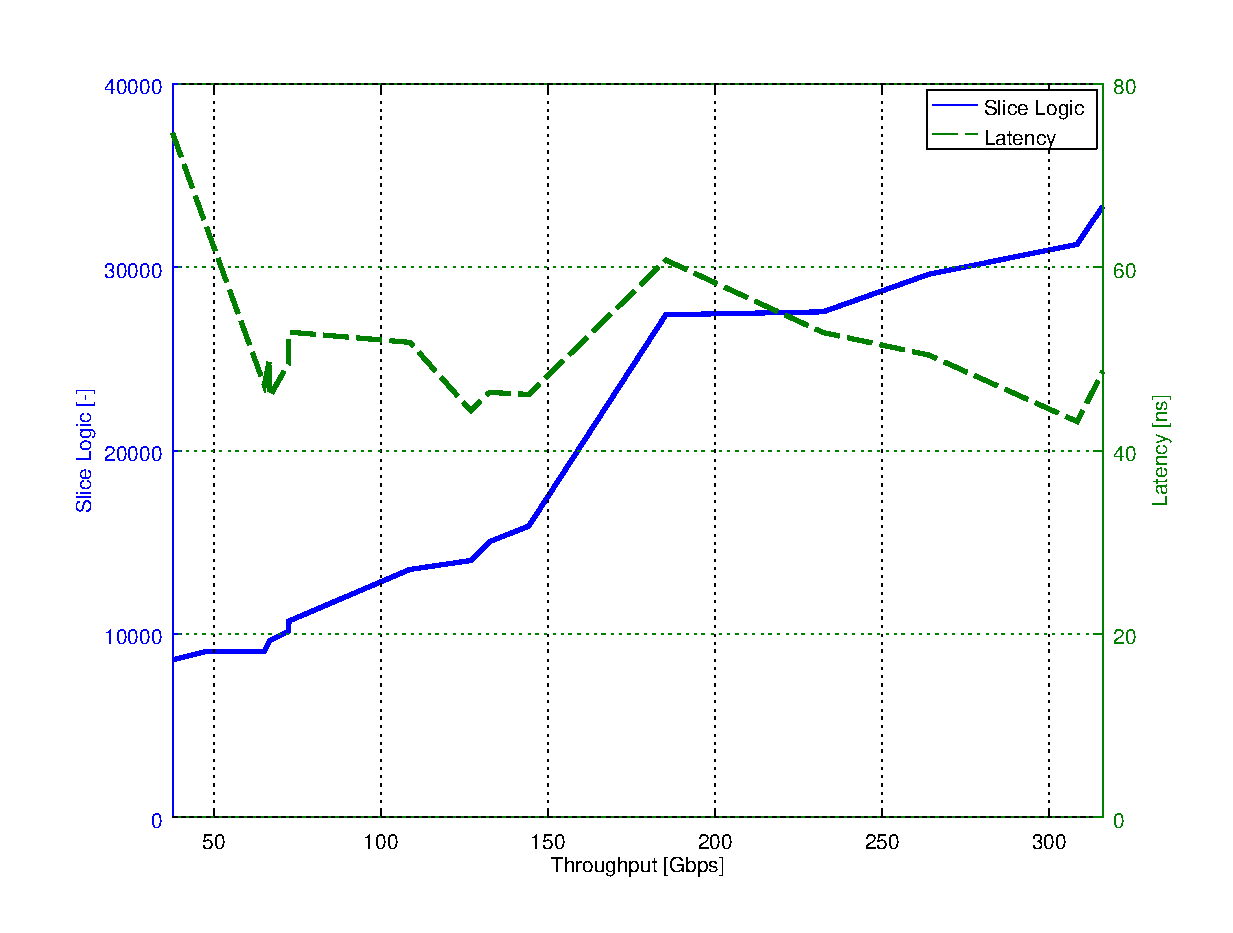
\includegraphics[scale=0.61]{chapters/pic/graphs/p4-pipeline/thr_slice_logic_pareto_ipv4_latency}
    \caption{IPv4 Filter - Pareto optimal solution optimized for throughput and resource utilization with corresponding latency.}
    \label{fig:ipv4ParetoLatency}
\end{figure}

\begin{figure}
    \centering
    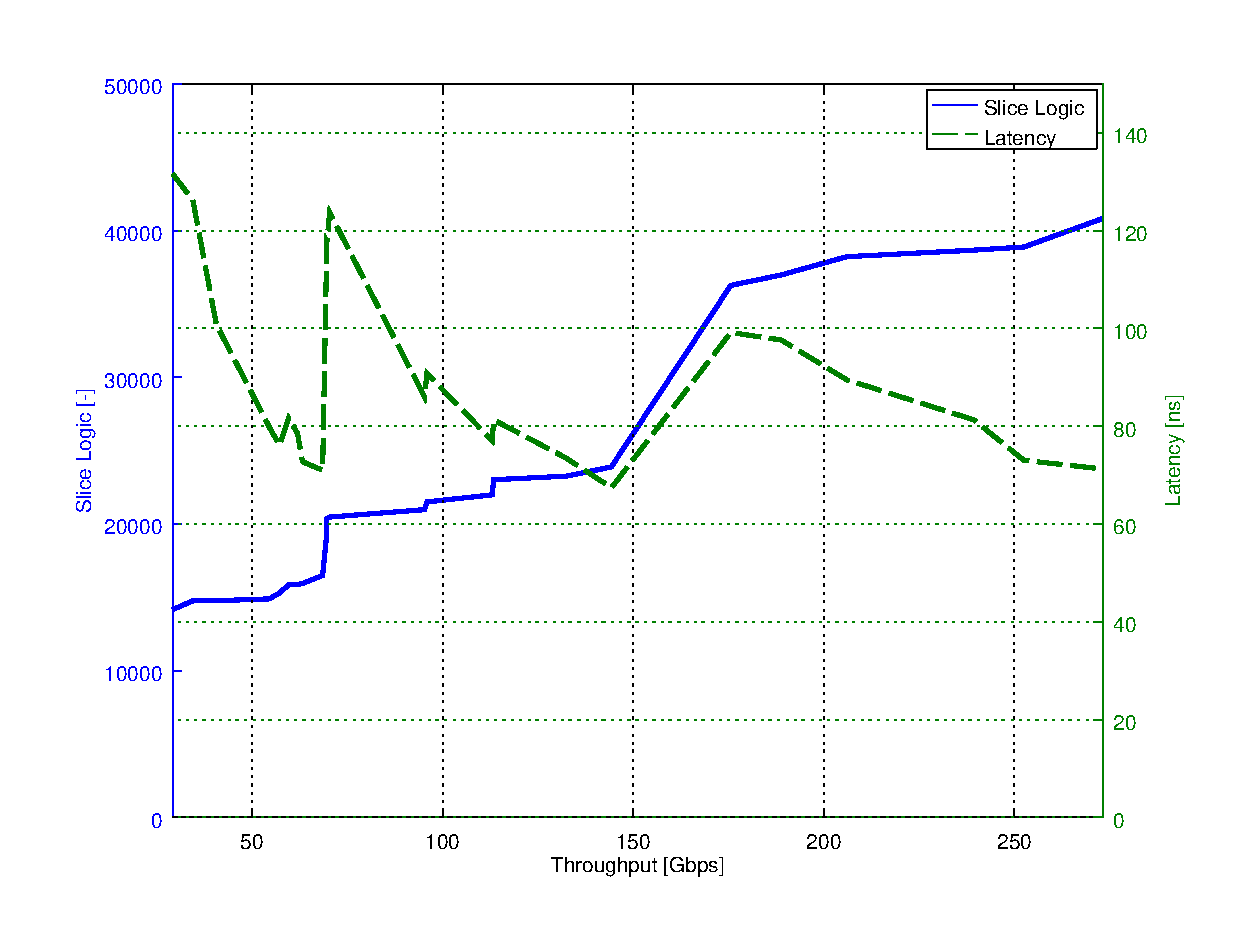
\includegraphics[scale=0.61]{chapters/pic/graphs/p4-pipeline/thr_slice_logic_pareto_ipv46_latency}
    \caption{IPv4+IPv6 Filter - Pareto optimal solution optimized for throughput and resource utilization with corresponding latency.}
    \label{fig:ipv46ParetoLatency}
\end{figure}

\begin{figure}
    \centering
    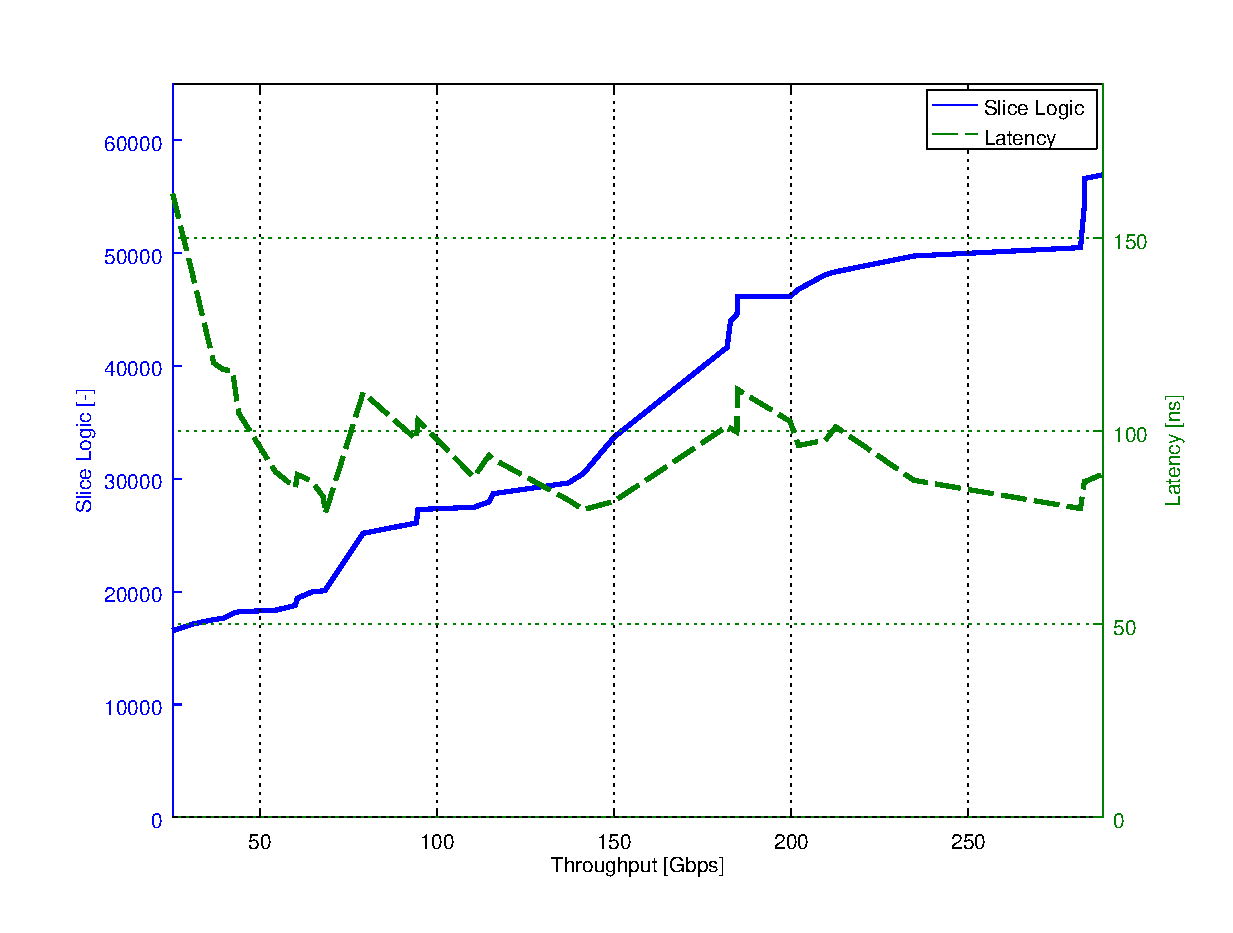
\includegraphics[scale=0.61]{chapters/pic/graphs/p4-pipeline/thr_slice_logic_pareto_full_latency}
    \caption{Full Filter - Pareto optimal solution optimized for throughput and resource utilization with corresponding latency.}
    \label{fig:fullParetoLatency}
\end{figure}

\begin{figure}
    \centering
    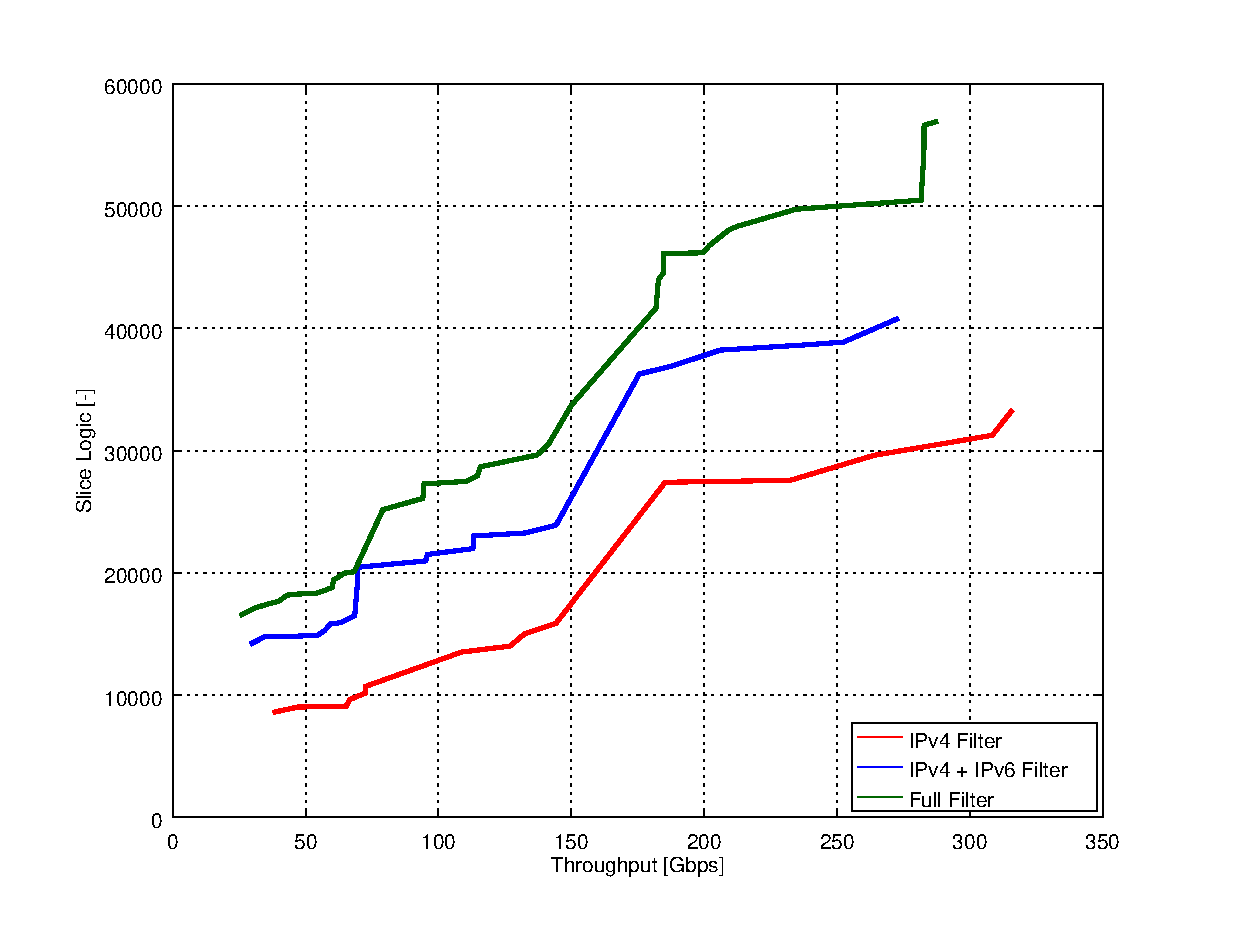
\includegraphics[scale=0.61]{chapters/pic/graphs/p4-pipeline/thr_slice_logic_pareto}
    \caption{Comparison of the FPGA resource utilization versus throughput Pareto sets for tested use cases.}
    \label{fig:useCasesParetoSets}
\end{figure}

In this section, we introduce resource utilization for individual use cases. The resource consumption can be divided into two  
parts --- resources of Match+Action pipeline and resources of parser/deparser.

Resource consumption of Match+Action pipeline is constant because this part of our architecture doesn't have any configurable
pipeline stages. The number of tables, routers, processed packets per one second and required resources after synthesis are shown in
Tab.~\ref{tab:resourcesMatchActionEngines}.
Each Match+Action table was configured to support 32 records in TCAM which is enough for validation of proposed architecture.
We provide required resources of \textit{Search Engines}, including TCAM parts, in Tab.~\ref{tab:resourcesTcamAndSearchEngine}. 
The TCAM part can be replaced by more effective or novel classification approach which leads to different resources.
All results are after synthesis for the Xilinx Virtex-7 XCVH580T FPGA using the Xilinx Vivado 2016.2 design tool. 

The parser/deparser resource utilization is fluctuating because both blocks have 
configurable pipeline modules (i.e., each configuration has different requirements on Slice Logic). 
We developed an automatic testing environment which is capable to translate P4 source, to configure generated VHDL code 
(i.e., the tool setups pipeline stages in parser and deparser), to start the synthesis, and to extract results from the synthesis log. 
This allows us to investigate complex set of possible solutions. 
However, the set of all solutions can be quite large (for complex P4 program) and it can be time consuming to process all 
possible configurations of pipeline stages. 
Due to this, we extend the tool with possibility to select a limited set of configurations which allows us to 
briefly inspect properties of generated devices. The tool was configured to test three different input data widths: 256, 512 and 1024. 
These parameters, data width and configuration of pipeline modules, generate a large space of available solutions.

\begin{table}[t]
    \centering
    \begin{tabular}{|l||c|c||c|c|}
        \hline
        \T \textbf{Project} & \textbf{Tables} & \textbf{Routers} & \textbf{Slice Logic\,[-]} & \textbf{Packet rate\,[Mpps]} \\ \hline\hline
        \T IPv4 Filter      &        2        &        1         &           1917            &             335              \\
        IPv4+IPv6 Filter    &        3        &        2         &           5781            &             339              \\
        Full Filter         &        3        &        2         &           6709            &             318              \\ \hline
    \end{tabular}
    \caption{Required resources of Match+Action engines.}
    \label{tab:resourcesMatchActionEngines}
\end{table}

We provide several graphs: three showing Pareto sets optimized for throughput and chip area without any regard to latency, 
and one for comparison of different Pareto sets of individual use cases. 
Graph of Pareto set for given use cases contains two axes.
The first axis shows required chip area in term of Slice Logic (number of used LUTs plus FlipFlops). 
The second axis shows corresponding latency of those solutions (optimized for throughput and chip area). 
Results of individual use cases are shown in Fig.~\ref{fig:ipv4ParetoLatency}, Fig.~\ref{fig:ipv46ParetoLatency} and 
Fig.~\ref{fig:fullParetoLatency}. It is also important to notice that provided solutions aren't globally optimal because 
our data set doesn't contain all possible solutions. However, the approach with limited configuration set allows to briefly inspect
properties of generated devices in a reasonable time.
Finally, the Fig.~\ref{fig:useCasesParetoSets} introduces comparison of Pareto sets optimized for throughput and chip area 
of provided use cases.

\begin{table}[h]
    \centering
    \begin{tabular}{|l||c|c||c|}
    	\hline
    	\T \textbf{Project} & \textbf{Search Engines\,[-]} & \textbf{BRAM\,[-]} & \textbf{TCAM Engines\,[-]} \\ \hline\hline
    	\T IPv4 Filter      &             956              &         1          &            527             \\
    	IPv4+IPv6 Filter    &             3529             &         1          &            2402            \\
    	Full Filter         &             3907             &         1          &            2406            \\ \hline
    \end{tabular}
    \caption{Resources of Search and TCAM engines; Values are summarized through all tables in given project and they are expressed 
        in term of Slice Logic.}
    \label{tab:resourcesTcamAndSearchEngine}
\end{table}

% Namerene vysledky z Vivado 2016.2
% IPv4 Filter
%================== 
% * IPv4 Filter table
%    + Match Engine --> 551 Lut, 341 Reg, BRAM 1
%    + TCAM --> 418 Lut, 109 Reg 
% * Drop table
%    + Match Engine --> 31 Lut, 33 Reg, BRAM 0
%    + TCAM --> 0 Lut, 0 Reg
%
% IPv4+IPv6 Filter
%==================
% * Drop table
%    + Match Engine --> 28 Lut, 33 Reg, BRAM 0
%    + TCAM --> 0 Lut, 0 Reg
% * Table IPv4 
%    + Match Engine --> 554 Lut, 345 Reg, BRAM 1
%    + TCAM --> 415 Lut, 109 Reg
% * Table IPv6
%    + Match Engine --> 1742 Lut, 827 Reg, BRAM 1
%    + TCAM --> 1577 Lut, 301 Reg
%
% IPv4+IPv6 Tag 
%==================
% * Drop table
%    + Match Engine --> 83 Lut, 34 Reg, BRAM 0
%    + TCAM -->  0 Lut, 0 Reg
% * Table IPv4
%    + Match Engine --> 624 Lut, 438 Reg, BRAM 1
%    + TCAM --> 418 Lut, 109 Reg
% * Tabel IPv6
%    + Match Engine --> 1808 Lut, 920 Reg, BRAM 1
%    + TCAM --> 1578 Lut, 301 Reg

\begin{figure}
    \centering
    \begin{subfigure}[b]{0.8\textwidth}
        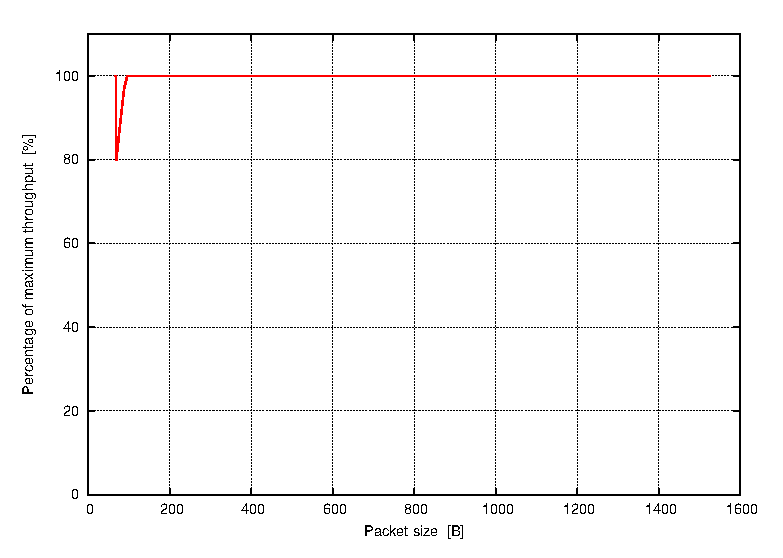
\includegraphics[width=\textwidth]{chapters/pic/graphs/h2rc-cases/ipv46_throughput}
        \caption{Percentage of maximum throughput.}
        \label{fig:bitThroughputIpv46}
    \end{subfigure}
    ~
    \begin{subfigure}[b]{0.8\textwidth}
        \includegraphics[width=\textwidth]{chapters/pic/graphs/h2rc-cases/ipv46_mpps_throughput}
        \caption{Packet rate.}
        \label{fig:packetThroughputIpv46}
    \end{subfigure}
    
    \caption{Throughput of generated IPv4 and IPv4+IPv6 Filter devices.}
    \label{fig:Ipv46Throughput}
\end{figure}

\begin{figure}
    \centering
    \begin{subfigure}[b]{0.8\textwidth}
        \includegraphics[width=\textwidth]{chapters/pic/graphs/h2rc-cases/full_throughput}
        \caption{Percentage of maximum throughput.}
        \label{fig:bitThroughputFull}
    \end{subfigure}
    ~
    \begin{subfigure}[b]{0.8\textwidth}
        \includegraphics[width=\textwidth]{chapters/pic/graphs/h2rc-cases/full_mpps_throughput}
        \caption{Packet rate.}
        \label{fig:packetThroughputFull}
    \end{subfigure}
    
    \caption{Throughput of generated Full Filter device.}
    \label{fig:FullThroughput}
\end{figure}

\begin{figure}
    \centering
    \includegraphics[scale=1.05]{chapters/pic/graphs/h2rc-cases/detail_throughput_ineff}
    \caption{Detail of IPv4, IPv4+IPv6 and Full Filter throughput for small packet sizes.}
    \label{fig:detailThroughputShortPacketLengts}
\end{figure}

\subsection{Throughput}
% * vysledky propustnosti jednotlivych reseni (vuci spirentu), sepsat jednotlive konfigurace ktere se povedly syntetizovat
% ** MPPS + Gbp
%
% Spirent generator byl nakonfigurovan, aby z 19 streamu
% * 6 streamu delal MPLS tag (31%)
% * 6 streamu delal VLAN tag (31%)

We measured throughput of all use cases in high-speed environment. We also created configuration tools capable to upload a user defined rule set.
The rule set was prepared for utilization of each implemented functionality. Therefore, we simulate a situation when 
incoming traffic is distributed across all supported functions. The Fig.~\ref{fig:Ipv46Throughput} shows percentage throughput
of IPv4 and IPv4+IPv6 Filter for generated traffic at speed of 100\,Gbps and a number of processed packets per one second. 
The Fig.~\ref{fig:FullThroughput} introduces the same but for the Full Filter use case.

All tests were performed against Spirent's Hypermetrics MX-100G-F1 module (SPT-N11U chassis).
The proposed results show that our architecture is capable to hit 100\,Gbps. However, there are some 
packet lengths when an inefficiency in deparser causes decrease of throughput. This inefficiency is related to insertion
of protocol header before payload because each Protocol Appender works with aligned data at zero offset. 
Therefore, this optimization leads to less effective usage of data bus (i.e., 64 bytes wide data bus cannot be shared by more packets) 
which leads to decrease of output throughput. 

The Full Filter has smaller throughput than IPv4 or IPv4+IPv6 Filter (compare short packet lengths in
Fig.~\ref{fig:detailThroughputShortPacketLengts}).
This is caused by insertion of four additional bytes (MPLS or VLAN tag) to a packet which leads to decrease of 
input throughput because deparser pipeline needs to be stalled during insertion. 
The Full Filter tags approximately 62\% of incoming traffic (31\% with MPLS tags and 31\% with VLAN tags).

\subsection{Generated Code vs. Total Lines of Code}
% * metrika poctu generovanych casti kodu vs. vsech radku (da se pouzit obsah souboru vivado.prj vs. vygenerovane soubory z p4-vhdl)
In this section, we introduce possible speedup in development of high-speed network devices. 
Reached results for individual use cases are shown in Tab.~\ref{tab:generatedVsTotalLines}.
The table contains compilation times of corresponding P4 source code (number of P4 source code lines is included). 
The \textbf{Generated lines} column expresses effort of the generator. For example, we generated 6283 lines of VHDL code from 91 lines
of P4 source code. The \textbf{Total lines} is a sum of generated lines and lines of library source code (FIFO, TCAM, and so on).
Table also shows that the generator produces approximately one third of each project. The VHDL code is generated from few lines
of P4 source code during two seconds.

% Vsechny casy jsou z prikazu date, real time, testovano na preklad4
% Generated lines (generovane radky v p4vhdl, bez library), Total lines (celkovy pocet radku vcetne knihovnich veci), 2570 radku vhdl_lib veci
\begin{table}[h]
    \centering
    \begin{tabular}{|l||c|c||c|c|}
        \hline
        \T \textbf{Project} & \textbf{P4 lines} & \textbf{Time\,[s]} & \textbf{Generated lines} & \textbf{Total lines} \\ \hline\hline
        \T IPv4 Filter      &        91         &       1.574        &           6283           &        24791         \\
        IPv4+IPv6 Filter    &        129        &       1.818        &           9888           &        28396         \\
        Full Filter         &        212        &       1.929        &          13824           &        32332         \\ \hline
    \end{tabular}
    \caption{Generated code versus total lines of code.}
    \label{tab:generatedVsTotalLines}
\end{table}

\section{Summary}
This chapter provides results of our architecture which was generated from abstract description in P4 language. 
The text introduces three use cases --- IPv4 Filter, IPv4+IPv6 Filter and Full Filter. 
These use cases demonstrate the flexibility and easy extensibility with support of new protocols and actions. 
All devices were generated in two seconds from
several lines of P4 source. This makes the development more effective. For example, developer can be focused on implementation of novel
hardware approaches related to classification because new module can be connected to the existing infrastructure. 
Text also provides Pareto sets optimized for throughput and resource requirements of individual use cases. 
Finally, all use cases were synthesized for COMBO-100G card and tested against Spirent network test device. 
Each use case is capable to hit throughput of 100\,Gbps at frequency of 225.8\,MHz on Xilinx Virtex-7 XCVH580T FPGA.
The results from this chapter are published in \cite{2016h2rc-p4,2016MicproP4}.
\widowpenalty=9999
\chapter{Conclusion}
\label{chap:conclusion}
% Summarize each chapter in one paragraph, point out the most important findings.
The aim of my \thesis{} is to provide the process of mapping from abstract language to the architecture of network device which is 
suitable for automatic generation and capable to hit processing speed of 100\,Gbps.

We propose the Parser-Deparser model. Our model of network device is based on the standard P4 model and it consists of three modules. 
The first module, parser, is used to break the incoming network data into individual header fields
(i.e., it has the same functionality like parser in P4 model).
The output of this module is a set of structured extracted fields, metadata and valid bits. All these inputs are passed
to the processing block which does not strictly define the structure of processing part 
(compared to the standard P4 model where the structure of processing part is given). 
Therefore, we are able to connect strong ideas of P4 model and rapid implementation of novel network functionality 
(e.g., pattern matching, new architectures of network devices, novel classification and so on). 
Finally, the last module, deparser, is used for construction of network packet back from protocol headers and valid bits.
This approach is general enough for variety of network applications. 
The Parser-Deparser model is capable to accommodate the P4 device model 
because the processing part allows mapping of Ingress Match+Action, Queues and/or Buffers and Egress Match+Action 
to predefined architecture.

We propose the architecture of our network pipeline which is suitable for automatic generation and capable to hit high-speeds. 
It is an example of the trade-off between complexity of high-speed network hardware blocks and transformation process. 
The proposed architecture contains several building blocks which are connected via predefined interfaces into deep high-speed pipeline.
We introduced the mapping from higher level (P4 language) to the architecture of parser, deparser, Match+Action tables,
Match+Action routers and Match+Action groups. The description on higher levels allows the user to be focused on implementation of 
network application without deep knowledge of underlying architecture. This approach was demonstrated on two examples --- 
(1)~transformation of P4 description to VHDL and (2)~extension of available action set with usage of current HLS tool where the
description of user action was provided in C/C++ language.
Our results shows that both approaches are capable to produce synthesizable code of a network device 
which is able to hit processing speed of 100\,Gbps.

The transformation from the P4 to VHDL was demonstrated on three use cases --- IPv4 Filter, IPv4+IPv6 Filter and Full Filter.
These use cases show the flexibility and easy extensibility of our architecture with new protocols and actions. The behavior of each use case
was described in P4 language and translated using our tool. We were able to reach the throughput in range from 77.6 to 100\,Gbps
and the frequency of 225.85\,MHz on Xilinx Virtex 7 XCVH580T FPGA. 

The transformation from C/C++ to VHDL was demonstrated on the extension of processing part with user defined actions.
The P4 language defines a fixed set of primitive actions. 
Unfortunately, this limitation is not suitable for future development because we typically need to extend the current action set with new actions 
(e.g., computation of advanced statistics, and so on). The user defined actions can be described in higher language which
is beneficial for fast development. Moreover, the source code of new action can by provided by administrator, mathematician or security expert.
The results of this research were verified in SDM \cite{KekelyPusKorenekSDM} project which is actively used for monitoring and protection 
of computer networks.

\section{Contributions of the Thesis}

The contributions of my \thesis{} are summarized in the following list:
\begin{enumerate}
    \item The modular architecture of network device which is suitable for generation of high-speed packet processing devices 
    from the abstract description.
    \item The structure and transformation process for individual parts of generated high-speed network device: 
    parser, Match+Action router, Match+Action table and deparser.
    \item The architecture of parallel Action Engine which is capable to process traffic at speed of 100\,Gbps. 
    The architecture of this engine was verified in SDM \cite{KekelyPusKorenekSDM} project.
    It is also capable to accommodate High-Level Synthesized engines which are described in C/C++ language.
    Results of this research are used in \cite{KekelyPusKorenekSdmIeeeTransactionComputerNetworks}.
    \item The tool, which generates the proposed architecture of network device from the abstract description in P4 language.
    \item Experimental results for parser, deparser and Match+Action processing pipeline. 
    Finally, the text provides three use cases which were tested 
    against Spirent's Hypermetrics MX-100G-F1 module (SPT-N11U chassis) at speed of 100\,Gbps. 
    Each use case was described in P4 language, translated to VHDL and tested in real hardware environment.
    The provided use cases demonstrate the flexibility and easy extensibility with support of new protocols and actions.
\end{enumerate}

\section{Future Work}
The author of the \thesis{} suggests to explore following:
\begin{itemize}
    \item Provide a general architecture of \textit{Check} engine.
    \item Investigate further optimizations of generated structure 
    (e.g., automatic detection of similar protocols which leads to optimization of PGR's structure).
    \item Provide an effective architecture of deparser block, capable to construct packets at speeds above 100\,Gbps.
    \item Provide architecture of more complex \textit{Search Engine} in Match+Action table.
    \item Extend the Match+Action table with advanced stateful processing (inspired by OpenState \cite{OpenStateSpec}).
    \item Provide a study of this technology for speeds beyond 100\,Gbps (e.g., for upcoming 400\,Gbps Ethernet standard).
    %\item Provide similar technology of processing pipeline for speeds up to 400\,Gbps. 
\end{itemize}

% % % % % % % % % % % % % % % % % % % % % % % % % % % % % % % % % % % % % % % % % % % % % % % % % % % % % % % % % % % %
% % % % Originalni text 
% % % % % % % % % % % % % % % % % % % % % % % % % % % % % % % % % % % % % % % % % % % % % % % % % % % % % % % % % % % %
%Chapter \ref{chap:stateOfTheArt} discusses the current approaches in the area of packet parsing, classification and data processing. 
%The chapter also introduces modern languages and abstractions of packet processing devices. We choose the P4 language as an input
%for our mapping process because this language provides good abstraction, is developed as open standard and is
%considered to be device and platform independent.
%
%Chapter \ref{chap:architectureOfNetworkDevice} introduces possible target architectures for mapping of P4 program. 
%Namely, the chapter introduces details about software implementations capable 
%to process 10\,Gbps, Network Processing Units (NPUs) capable to process traffic at speed of 40\,Gbps, and Field Programmable Gate Array (FPGA)
%which is capable to process data at speed of 100\,Gbps.
%We select the FPGA as our target platform because it connects parallel nature of hardware with flexibility of software. 
%The chapter also introduces the idea of mapping to the architecture of network device which is based on Parser-Deparser model.
%The proposed architecture consists of several building blocks which are connected to processing pipeline where some 
%parts of these blocks are generated, some configured and some instantiated.
%
%Chapter \ref{chap:parserDeparserArchitecture} introduces detailed architecture and transformation process from P4 language to parser and deparser 
%blocks. 
%%Both blocks are carefully designed to meet a trade-off between complexity of hardware and generator. 
%Parser consists of pipeline modules and Protocol Analyzers which are connected via common interface. 
%The same architecture is used in the case of deparser.
%This approach is beneficial during generation of mentioned blocks because the structure of generated hardware is homogenous. 
%The text provides the algorithms for transformation from P4 to the structure of parser and deparser.
%We also compared generated to hand-written parsers. The cost for automatic generation is roughly doubled latency and chip area. 
%Finally, we connected parser and deparser together and perform throughput tests in real hardware platform. 
%Results show that generated blocks are capable to hit speed of 100\,Gbps, except some packet lengths when the inefficiency in deparser shows up. 
%The text also proposes required changes to meet the full throughput of 100\,Gbps.
%
%Chapter \ref{chap:matchActionProcessing} introduces results of our research regarding the Match+Action processing pipeline with further
%details about transformation algorithm and generated architecture. We introduced mapping from P4 language to 
%Match+Action groups, Match+Action tables and Match+Action routers which are the main building blocks of our processing pipeline. 
%All mentioned modules use the common communication interface which is beneficial during automatic generation.
%The text also provides details about usage of current HLS tool which can be used for easy extension of available actions in Action Engine.
%That is, we can provide abstract definition of user-defined engines in C/C++ and translate this code to HDL language. 
%After that, the generated code is connected into existing infrastructure which is capable to process data at speed of 100\,Gbps. 
%
%Finally, Chapter \ref{chap:use-case-study} provides results for three use cases where each use case was generated from P4 description.
%We provided results of required resources, throughput and number of generated lines, together with required time for compilation.
%Each use case meet throughput in range from 77.6 to 100\,Gbps at frequency of 225.8\,MHz on Xilinx Virtex-7 XCVH580T FPGA.

%------------------------------------------------------------------------------------------
% Use bibtex to produce bibliography used in the thesis, except for your own publications
%------------------------------------------------------------------------------------------
\bibliographystyle{iso690}
%\bibliographystyle{abbrv}
% \cleardoublepage\phantomsection\addcontentsline{toc}{chapter}{\protect\numberline{}{Bibliography}}
\bibliography{bibliography}

%-----------------------
% Publications of the author
% Start every record with A.#
\newcounter{MyPublRefCount}
\setcounter{MyPublRefCount}{0}
\def\bibauthor#1{\addtocounter{MyPublRefCount}{1}\bibitem[A.\theMyPublRefCount]{#1}}

% list your own books or papers in refereed journals or conference proceedings
% or chapters in scientific monographies that are RELEVANT FOR YOUR THESIS
\renewcommand\bibname{Reviewed Publications of the Author Relevant to the Thesis}
% \cleardoublepage\phantomsection\addcontentsline{toc}{chapter}{\protect\numberline{}{Reviewed Relevant Publications of the Author}}
\begin{thebibliography}{A.9}%here fill-in the longest label in the list of your publications
\itemsep=0pt
%
%----------------------------------------------------
% \bibauthor{ID}. Cite as \cite{ID}.

\section*{Reviewed publications}
\bibauthor{2016fccm-p4-parser}
P. Ben\'{a}\v{c}ek, V. Pu\v{s} and H. Kub\'{a}tov\'{a}.
\newblock \textit{P4-to-VHDL: Automatic Generation of 100Gbps Packet Parsers}.
\newblock IEEE 24\textsuperscript{th} Annual International Symposium on Field-Programmable Custom Computing Machines (FCCM2016), Washington D.C., USA, 
\newblock 2016.

\bibauthor{2015h2rc-p4-parser}
P. Ben\'{a}\v{c}ek, V. Pu\v{s} and H. Kub\'{a}tov\'{a}.
\newblock \textit{Automatic Generation of 100 Gbps Packet Parsers from P4 Description}.
\newblock First International Workshop on Heterogeneous High-performance Reconfigurable Computing, Austin, TX, USA, 
\newblock 2015.

\bibauthor{2014binder}
P. Ben\'{a}\v{c}ek, H. Kub\'{a}tov\'{a} and V. Pu\v{s}.
\newblock \textit{Architecture of Effective High-Speed Network Stream Merger}.
\newblock Digital System Design (DSD), 17\textsuperscript{th} Euromicro Conference on Digital System Design, pp. 459--464, Verona, Italy,
\newblock 2014.

\bibauthor{2014hls-instructions}
P. Ben{\'a}{\v{c}}ek and V. Pu{\v{s}}.
\newblock \textit{Application specific processor with high-level synthesized instructions}.
\newblock ACM/SIGDA international symposium on Field-Programmable Gate Arrays, pp. 246--246, Monterey, CA, USA,
\newblock 2014.

\bibauthor{2014sdmcpd-monterey}
P. Ben\'{a}\v{c}ek, T. \v{C}ejka, H. Kub\'{a}tov\'{a} and R. Bla\v{z}ek.
\newblock \textit{Change-Point Detection Method on 100 Gb/s Ethernet Interface}.
\newblock ACM/IEEE Symposium on Architectures for Networking and Communications Systems, Marina del Rey, CA, USA,
\newblock 2014.

\bibauthor{2014sdmmemincs}
P. Ben\'{a}\v{c}ek, T. \v{C}ejka, H. Kub\'{a}tov\'{a}, L. Kekely and R. Bla\v{z}ek.
\newblock \textit{FPGA Accelerated Change-Point Detection Method for 100 Gb/s Networks}.
\newblock Doctoral Workshop on Mathematical and Engineering Methods in Computer Science, Tel\v{c}, Czech Republic,
\newblock 2014.

\bibauthor{2016h2rc-p4}
P. Ben\'{a}\v{c}ek, V. Pu\v{s} and P. Ka\v{s}tovsk\'y.
\newblock \textit{P4-to-FPGA: High Performance Reconfigurable Networking (poster)}.
\newblock Second International Workshop on Heterogeneous High-performance Reconfigurable Computing, Salt Lake City, UT, USA,
\newblock 2016.

\bibauthor{2016stanford-p4-demo}
P. Ben{\'a}{\v{c}}ek and V. Pu{\v{s}} 
\newblock \textit{P4-to-VHDL: Generating High Speed Network Devices (poster)}. 
\newblock P4 Workshop, Stanford, California, USA, 
\newblock 2016. Available from: \url{https://www.liberouter.org/wp-content/uploads/2016/06/poster\_p4\_06\_2016.pdf}

\bibauthor{kekely2014trade}
L. Kekely, V. Pu\v{s}, P. Ben{\'a}\v{c}ek and J. Ko\v{r}enek.
\newblock \textit{Trade-offs and progressive adoption of FPGA acceleration in network traffic monitoring}.
\newblock Field Programmable Logic and Applications (FPL), 24\textsuperscript{th} International Conference, pp. 1--4, Munich, Germany,
\newblock 2014.
\smallskip \\ \smallskip The paper has been cited in:
\begin{itemize}
    \item D. Grochol, L. Sekanina, M. \v{Z}\'{a}dn\'{i}k, J. Ko\v{r}enek. \textit{Evolutionary circuit design for fast FPGA-based classification of network application protocols}. 
    Applied Soft Computing, Volume 38, January 2016, pp. 933-941.
    \item L. Tang, J. Yan, Z. Sun, T. Li, M. Zhang. \textit{Towards high-performance packet processing on commodity multi-cores: current issues and future directions}.
    Research Paper Special Focus On Future Internet Architecture And Protocol Science China Information Sciences, December 2015, Volume 58, Issue 12, pp. 1-16.
\end{itemize}

\section*{Submitted publications}
\bibauthor{2016MicproP4}
P. Ben\'{a}\v{c}ek, H. Kub\'{a}tov\'{a} and V. Pu\v{s}.
\newblock \textit{P4-to-VHDL: Automatic Generation of High-Speed Input and Output Network Blocks}.
\newblock Microprocessors and Microsystems, Elsevier Journal, 2016.

%%%%%%%%%%%%%%%%%%%%%%%%%%%%%%%%%%%%%%%%%%%%%%%%%%%%%%%%%%%%%%%%%%%%%%%%%%%%%%%
%Example of the citation                                                      %
%%%%%%%%%%%%%%%%%%%%%%%%%%%%%%%%%%%%%%%%%%%%%%%%%%%%%%%%%%%%%%%%%%%%%%%%%%%%%%%
%\bibitem{YOURPUBL-ZZZ1}
%Gortz, R.; T\"ol\"ok\"o, F.
%\newblock On the Carpathian Castle.
%\newblock In: \textit{Transylvanian Journal of \dots}.
%\newblock Werst, Romania,
%\newblock 2010.
%% nepovinny blok s citaci:
%% ************* 
%\bigskip \\ \smallskip The paper has been cited in:
%\begin{itemize}
%\item Nov\'ak\r{u}, \v{S}. Carpathian Castle Revealed. \textit{International Symposium on Carpathian Legends}. 1:319--323, 2010.
%\end{itemize}
% *************
\end{thebibliography}

\renewcommand\bibname{Remaining Publications of the Author Relevant to the Thesis}
% \cleardoublepage\phantomsection\addcontentsline{toc}{chapter}{\protect\numberline{}{Remaining Relevant Publications of the Author}}
\begin{thebibliography}{A.9}%here fill-in the longest label in the list of your publications
%----------------------------------------------------

\bibauthor{2016benacek-phd-minimum}
P. Ben\'{a}\v{c}ek.
\newblock \textit{Methodology for Analysis of High-Speed Networks}. 
\newblock Ph.D. Minimum Thesis,  Faculty of Information Technology, Czech Technical University in Prague, Czech Republic, 
\newblock 2014.

\bibauthor{2016pesw}
P. Ben\'{a}\v{c}ek, H. Kub\'{a}tov\'{a} and V. Pu\v{s}.
\newblock \textit{P4-to-FPGA: Translating P4 to VHDL}.
\newblock The 4\textsuperscript{th} Prague Embedded Systems Workshop (PESW 2016), ISBN 978-80-01-05984-5, Roztoky, Czech Republic,
\newblock 2016.

\bibauthor{2016cesnet-p4}
P. Ben{\'a}{\v{c}}ek and V. Pu{\v{s}} 
\newblock \textit{The P4 Language as the Future of SDN (CZ)}. 
\newblock CESNET blog, 
\newblock 2016. Available from: \url{https://www.cesnet.cz/2016/01/jazyk-p4/}

\bibauthor{2016root-p4}
P. Ben{\'a}{\v{c}}ek and V. Pu{\v{s}} 
\newblock \textit{The P4 Language as the Future of SDN (CZ)}. 
\newblock root.cz (part 1 and part 2), 
\newblock 2016. Available from: 
\newblock Part 1 - \url{http://www.root.cz/clanky/jazyk-p4-jako-budoucnost-sdn/}, 
\newblock Part 2 - \url{http://www.root.cz/clanky/jazyk-p4-jako-budoucnost-sdn-dokonceni/}

% Switch language to czech, print some publications and swithch it back to the english :)
\selectlanguage{czech}

\bibauthor{benacekpad2012}
P. Ben\'{a}\v{c}ek.
\newblock \textit{Anal\'{y}za rychl\'{y}ch s\'{i}\v{t}ov\'{y}ch p\v{r}enos\r{u}}.
\newblock \v{C}esko-slovensk\'{y} semin\'{a}\v{r} PAD, pp. 9--12, ISBN 978-80-01-05106-1, Milovy ve \v{Z}\v{d}\'{a}rsk\'{y}ch vr\v{s}\'{i}ch, \v{C}esk\'{a} republika,
\newblock 2012.
\newblock \textit{The paper was awarded as the best publication of first-year students.}

\bibauthor{benacekarchitektura}
P. Ben\'{a}\v{c}ek.
\newblock \textit{Architektura pro m\v{e}\v{r}en\'{i} v re\'{a}ln\'{e}m \v{c}ase na vysokorychlostn\'{i}ch s\'{i}t\'{i}ch}.
\newblock \v{C}esko-slovensk\'{y} semin\'{a}\v{r} PAD, pp. 45--50, ISBN 978-80-261-0270-0, Tepl\'{a}, \v{C}esk\'{a} republika,
\newblock 2013.

\bibauthor{benavcekreal}
P. Ben\'{a}\v{c}ek.
\newblock \textit{Real-time Network Measurement for High-Speed Networks}.
\newblock The 1\textsuperscript{st} Embedded Systems Workshop (ESW), Teme\v{s}v\'{a}r, Czech Republic,
\newblock 2013.

\selectlanguage{UKenglish}

%%%%%%%%%%%%%%%%%%%%%%%%%%%%%%%%%%%%%%%%%%%%%%%%%%%%%%%%%%%%%%%%%%%%%%%%%%%%%%%
%Example of the citation                                                      %
%%%%%%%%%%%%%%%%%%%%%%%%%%%%%%%%%%%%%%%%%%%%%%%%%%%%%%%%%%%%%%%%%%%%%%%%%%%%%%%
%\bibitem{YOURPUBL-MINIMUM}
%Gortz, R.
%\newblock \textit{MINIMUM TITLE}.
%\newblock Ph.D. Minimum Thesis, Faculty of Information Technology,
%\newblock Prague, Czech Republic,
%\newblock 2010.
%% nepovinny blok s citaci:
%% ************* 
%\bigskip \\ \smallskip The paper has been cited in:
%\begin{itemize}
%\item L\'ef\`evre, \c{C}. \textit{Le Ch\^ateau des Carpathes : Le fin alternatif d\'ecouvert~!}, \dots.
%\item Q. Ma\~nana. \dots
%\item H. Erd\H{o}s. \dots
%\item \r{A}. S\o renson. \dots
%\end{itemize}
% *************
\end{thebibliography}

\renewcommand\bibname{Remaining Publications of the Author}
% \cleardoublepage\phantomsection\addcontentsline{toc}{chapter}{\protect\numberline{}{Remaining Publications of the Author}}
\begin{thebibliography}{A.9}%here fill-in the longest label in the list of your publications
%----------------------------------------------------

\bibauthor {presentcipher}
P. Ben\'{a}\v{c}ek and M. Novotn\'{y}.
\newblock \textit{Implementing Brute-Force Attack on PRESENT Cipher}.
\newblock Digital System Design (DSD), 13\textsuperscript{th} Euromicro Conference on Digital System Design, pp. 51--52, Linz, Austria,
\newblock 2010.

\bibauthor{cometreport}
P. Ben\'{a}\v{c}ek, T. \v{C}ejka, \v{S}. Friedl and R. Krej\v{c}\'{i}.
\newblock \textit{COMET - COMBO Ethernet Tester}.
\newblock Annual report, CESNET z.s.p.o., Prague, Czech Republic,
\newblock 2013.
\newblock Available from: \url{http://www.cesnet.cz/wp-content/uploads/2013/03/comet.pdf}

%%%%%%%%%%%%%%%%%%%%%%%%%%%%%%%%%%%%%%%%%%%%%%%%%%%%%%%%%%%%%%%%%%%%%%%%%%%%%%%
%Example of the citation                                                      %
%%%%%%%%%%%%%%%%%%%%%%%%%%%%%%%%%%%%%%%%%%%%%%%%%%%%%%%%%%%%%%%%%%%%%%%%%%%%%%%
%\bibitem{YOURPUBL-P2}
%Gortz, R.
%\newblock Another publication.
%\newblock \textit{36\textsuperscript{th} International Conference on \dots}. pp. 19--24, \v{S}trbsk\'e pleso, Slovak Republic,
%\newblock 2010.
%*************************************************************************
\end{thebibliography}

\renewcommand\bibname{Evaluation Activities}
% \cleardoublepage\phantomsection\addcontentsline{toc}{chapter}{\protect\numberline{}{Remaining Publications of the Author}}
\begin{thebibliography}{A.9}%here fill-in the longest label in the list of your publications
%----------------------------------------------------
\bibauthor{reconfig2016}
Conference Programme Committee member in the 
\textit{Track on Reconfigurable Computing for Networks and Communications.}
\newblock International Conference on Reconfigurable Computing and FPGAs (ReConFig'2016), Cancum, Mexico,
\newblock 2016.
\newblock Available from: \url{http://www.reconfig.org/index.php?option=com\_content&view=article&id=6&Itemid=134}

\bibauthor{jpdc-2016}
Review of article for the \textit{Journal of Parallel and Distributed Computing}. 
\newblock Article in journal, ISSN 0743-7315,
\newblock 2016.
\newblock Available from: \url{http://www.journals.elsevier.com/journal-of-parallel-and-distributed-computing}

%%%%%%%%%%%%%%%%%%%%%%%%%%%%%%%%%%%%%%%%%%%%%%%%%%%%%%%%%%%%%%%%%%%%%%%%%%%%%%%
%Example of the citation                                                      %
%%%%%%%%%%%%%%%%%%%%%%%%%%%%%%%%%%%%%%%%%%%%%%%%%%%%%%%%%%%%%%%%%%%%%%%%%%%%%%%
%\bibitem{YOURPUBL-P2}
%Gortz, R.
%\newblock Another publication.
%\newblock \textit{36\textsuperscript{th} International Conference on \dots}. pp. 19--24, \v{S}trbsk\'e pleso, Slovak Republic,
%\newblock 2010.
%*************************************************************************
\end{thebibliography}


%-----------------------
% Appendis 
%\appendix
%\include{chapters/appendix1}

% % Add the index if it is requested above
% \ifx\printindex\undefined\relax\else\cleardoublepage\phantomsection\addcontentsline{toc}{chapter}{\protect\numberline{}{Index}}\fi
% \ifx\printindex\undefined\relax\else\printindex\fi
\end{document}
